% !TeX encoding = UTF-8
% !TeX program = xelatex
% !TeX spellcheck = en_US

\documentclass[degree = bachelor, draft]{thuthesis}
% 学位 degree:
%   doctor | master | bachelor | postdoc
% 学位类型 degree-type:
%   academic(默认)| professional
% 语言 language
%   chinese(默认)| english
% 字体库 fontset
%   windows | mac | fandol | ubuntu
% 建议终版使用 Windows 平台的字体编译

% 论文基本配置,加载宏包等全局配置
% !TeX root = ./thuthesis-example.tex

% 论文基本信息配置

\thusetup{
  %******************************
  % 注意:
  %   1. 配置里面不要出现空行
  %   2. 不需要的配置信息可以删除
  %   3. 建议先阅读文档中所有关于选项的说明
  %******************************
  %
  % 输出格式
  %   选择打印版(print)或用于提交的电子版(electronic),前者会插入空白页以便直接双面打印
  %
  output = print,
  %
  % 标题
  %   可使用“\\”命令手动控制换行
  %
  title  = {基于物理模拟的正颌手术术后外形预测},
  title* = {Physics-based Prediction of Post-surgery Shape in Orthognathic Surgery},
  %
  % 学科门类
  %   1. 学术型
  %      - 中文
  %        需注明所属的学科门类,例如:
  %        哲学、经济学、法学、教育学、文学、历史学、理学、工学、农学、医学、
  %        军事学、管理学、艺术学
  %      - 英文
  %        博士:Doctor of Philosophy
  %        硕士:
  %          哲学、文学、历史学、法学、教育学、艺术学门类,公共管理学科
  %          填写“Master of Arts“,其它填写“Master of Science”
  %   2. 专业型
  %      直接填写专业学位的名称,例如:
  %      教育博士、工程硕士等
  %      Doctor of Education, Master of Engineering
  %   3. 本科生不需要填写
  %
  % degree-category  = {工学硕士},
  % degree-category* = {Master of Science},
  %
  % 培养单位
  %   填写所属院系的全名
  %
  department = {软件学院},
  %
  % 学科
  %   1. 研究生学术型学位,获得一级学科授权的学科填写一级学科名称,其他填写二级学科名称
  %   2. 本科生填写专业名称,第二学位论文需标注“(第二学位)”
  %
  discipline  = {软件工程},
  discipline* = {Software Engineering},
  %
  % 专业领域
  %   1. 设置专业领域的专业学位类别,填写相应专业领域名称
  %   2. 2019 级及之前工程硕士学位论文,在 `engineering-field` 填写相应工程领域名称
  %   3. 其他专业学位类别的学位论文无需此信息
  %
  % professional-field  = {计算机技术},
  % professional-field* = {Computer Technology},
  %
  % 姓名
  %
  author  = {李钦},
  author* = {Li Qin},
  %
  % 指导教师
  %   中文姓名和职称之间以英文逗号“,”分开,下同
  %
  supervisor  = {徐枫, 副教授},
  supervisor* = {Professor Xu Feng},
  %
  % 副指导教师
  %
  % associate-supervisor  = {陈文光, 教授},
  % associate-supervisor* = {Professor Chen Wenguang},
  %
  % 联合指导教师
  %
  % co-supervisor  = {某某某, 教授},
  % co-supervisor* = {Professor Mou Moumou},
  %
  % 日期
  %   使用 ISO 格式;默认为当前时间
  %
  % date = {2019-07-07},
  %
  % 是否在中文封面后的空白页生成书脊(默认 false)
  %
  include-spine = false,
  %
  % 密级和年限
  %   秘密, 机密, 绝密
  %
  % secret-level = {秘密},
  % secret-year  = {10},
  %
  % 博士后专有部分
  %
  % clc                = {分类号},
  % udc                = {UDC},
  % id                 = {编号},
  % discipline-level-1 = {计算机科学与技术},  % 流动站(一级学科)名称
  % discipline-level-2 = {系统结构},          % 专业(二级学科)名称
  % start-date         = {2011-07-01},        % 研究工作起始时间
}

% 载入所需的宏包

% 定理类环境宏包
\usepackage{amsthm}
% 也可以使用 ntheorem
% \usepackage[amsmath,thmmarks,hyperref]{ntheorem}

\thusetup{
  %
  % 数学字体
  % math-style = GB,  % GB | ISO | TeX
  math-font  = xits,  % stix | xits | libertinus
}

% 可以使用 nomencl 生成符号和缩略语说明
\usepackage{nomencl}
\makenomenclature

% 表格加脚注
\usepackage{threeparttable}

% 表格中支持跨行
\usepackage{multirow}

% 固定宽度的表格。
% \usepackage{tabularx}

% 跨页表格
\usepackage{longtable}

% 算法
\usepackage{algorithm}
\usepackage{algorithmic}

% 量和单位
\usepackage{siunitx}

% 参考文献使用 BibTeX + natbib 宏包
% 顺序编码制
% \usepackage[sort]{natbib}
% \bibliographystyle{thuthesis-numeric}

% 著者-出版年制
% \usepackage{natbib}
% \bibliographystyle{thuthesis-author-year}

% 本科生参考文献的著录格式
\usepackage[sort]{natbib}
\bibliographystyle{thuthesis-bachelor}

% 参考文献使用 BibLaTeX 宏包
% \usepackage[style=thuthesis-numeric]{biblatex}
% \usepackage[style=thuthesis-author-year]{biblatex}
% \usepackage[style=thuthesis-bachelor]{biblatex}
% \usepackage[style=apa]{biblatex}
% \usepackage[style=mla-new]{biblatex}
% 声明 BibLaTeX 的数据库
% \addbibresource{ref/refs.bib}

% 定义所有的图片文件在 figures 子目录下
\graphicspath{{figures/}}

% 数学命令
\makeatletter
\newcommand\dif{%  % 微分符号
  \mathop{}\!%
  \ifthu@math@style@TeX
    d%
  \else
    \mathrm{d}%
  \fi
}
\makeatother

\usepackage{physics}

% hyperref 宏包在最后调用
\usepackage{hyperref}


\begin{document}

% 封面
\maketitle

% 学位论文指导小组、公开评阅人和答辩委员会名单
% 本科生不需要
% % !TeX root = ../thuthesis-example.tex

\begin{committee}[name={学位论文指导小组、公开评阅人和答辩委员会名单}]

  \newcolumntype{C}[1]{@{}>{\centering\arraybackslash}p{#1}}

  \section*{指导小组名单}

  \begin{center}
    \begin{tabular}{C{3cm}C{3cm}C{9cm}@{}}
      李XX & 教授     & 清华大学 \\
      王XX & 副教授   & 清华大学 \\
      张XX & 助理教授 & 清华大学 \\
    \end{tabular}
  \end{center}

  \section*{公开评阅人名单}

  \begin{center}
    \begin{tabular}{C{3cm}C{3cm}C{9cm}@{}}
      刘XX & 教授   & 清华大学                    \\
      陈XX & 副教授 & XXXX大学                    \\
      杨XX & 研究员 & 中国XXXX科学院XXXXXXX研究所 \\
    \end{tabular}
  \end{center}

  \section*{答辩委员会名单}

  \begin{center}
    \begin{tabular}{C{2.75cm}C{2.98cm}C{4.63cm}C{4.63cm}@{}}
      主席 & 赵XX                  & 教授                    & 清华大学       \\
      委员 & 刘XX                  & 教授                    & 清华大学       \\
           & \multirow{2}{*}{杨XX} & \multirow{2}{*}{研究员} & 中国XXXX科学院 \\
           &                       &                         & XXXXXXX研究所  \\
           & 黄XX                  & 教授                    & XXXX大学       \\
           & 周XX                  & 副教授                  & XXXX大学       \\
      秘书 & 吴XX                  & 助理研究员              & 清华大学       \\
    \end{tabular}
  \end{center}

\end{committee}

% 也可以导入 Word 版转的 PDF 文件
% \begin{committee}[file=figures/committee.pdf]
% \end{committee}


% 使用授权的说明
% \copyrightpage
% 将签字扫描后授权文件 scan-copyright.pdf 替换原始页面
% \copyrightpage[file=scan-copyright.pdf]

\frontmatter
% % !TeX root = ../thuthesis-example.tex

% 中英文摘要和关键字

\begin{abstract}
  全球范围内,每年都有许多患者因患有颅颌面畸形而饱受困扰。
  这些畸形不仅可能影响患者的基本生理功能,还会对其心理健康和社会交际产生负面影响。
  正颌手术是治疗颅颌面畸形的重要手段,通过手术可以显著改善患者的生理功能和面部外观。
  术前决策过程中,术后外观预测是患者和医生关注的核心问题,对手术方案的选择至关重要。

  传统的术后外观预测方法主要依赖于医生的主观经验,这种做法往往缺乏客观性和可度量性,且因个体差异较大,预测结果可能不够精确。
  为克服这些限制,本研究提出了一种基于物理模拟的正颌手术术后外观预测新策略。
  通过结合高精度的骨骼和面部重建算法以及生物力学仿真模型,本研究旨在提供更为客观、精确的术后外观预测方法。

  具体来说,本研究实现了两个核心步骤:
  1. 实现了一种高精度且自动化的骨骼和面部重建算法。
  该算法结合了刚性和非刚性配准方法,通过处理患者头部的 CT 影像数据,能够生成高分辨率和一致拓扑的三维模型。
  此方法不仅具有高度的准确性,还显著提升了自动化水平,减少了人工干预所带来的误差。
  2. 利用符合生物力学原理的高效质点-张量模型,对手术后软组织的形态变化进行仿真。
  该模型考虑了软组织的生物力学特性,通过模拟手术过程中骨骼移动对软组织的牵拉和压迫作用,能够精确预测手术后的面部形态变化。
  % 仿真过程中,采用并行计算技术,显著提高了计算效率,确保在短时间内获得高质量的预测结果。

  实验结果显示,本研究提出的预测策略能够有效地预测正颌手术的术后外观,具备较高的精确度和计算效率。
  与传统方法相比,该策略在客观性和准确性方面具有显著优势,为正颌手术的术后外观预测提供了可行的方法,并有潜力成为临床实践中有效的辅助决策工具。
  未来,本研究还将进一步优化模型,结合更多的生物力学数据和临床案例,以提升预测模型的准确性和实用性。

  % 关键词用“英文逗号”分隔,输出时会自动处理为正确的分隔符
  \thusetup{
    keywords = {生物力学建模, 正颌手术模拟, 有限元模型},
  }
\end{abstract}

\begin{abstract*}
  Globally, many patients suffer from craniofacial deformities each year, impacting not only their basic physiological functionalities but also their mental health and social interactions.
  Orthognathic surgery is a crucial method for treating these deformities, significantly enhancing both physiological functionalities and facial appearance.
  In the pre-operative decision-making process, predicting post-operative appearance is a core concern for both patients and doctors and is essential for selecting the appropriate surgical plan.

  Traditional methods for predicting post-operative appearance primarily rely on the subjective experience of doctors.
  This approach often lacks objectivity and measurability, and due to individual differences, the predictions may not be sufficiently accurate.
  To overcome these limitations, this research proposes a new strategy based on physical simulation for predicting post-operative appearance.
  By combining high-precision skeletal and facial reconstruction algorithms with biomechanical models, this research aims to provide a more objective and accurate method for prediction.

  Specifically, this research achieves two core steps:
  1. A high-precision, automatic algorithm for skeletal and facial reconstruction.
  This algorithm combines rigid and non-rigid registration methods, processes CT imaging data of patients' heads, and generates high-resolution three-dimensional models with consistent topology.
  This method not only achieves high accuracy but also significantly enhances automation, reducing errors caused by manual intervention.
  2. An efficient mass-tensor model that adheres to biomechanical principles is used to simulate the morphological changes of soft tissues post-surgery.
  This model considers the biomechanical properties of soft tissues and can accurately predict post-operative facial morphological changes by simulating the effects of bone movement on soft tissues during surgery.

  The experimental results demonstrate that the proposed prediction strategy can effectively predict the post-operative appearance of orthognathic surgery with high accuracy and computational efficiency.
  Compared to traditional methods, this strategy offers significant advantages in terms of objectivity and accuracy, providing a feasible method for predicting post-operative appearance in orthognathic surgery and the potential to become an effective auxiliary decision-making tool in clinical practice.
  In the future, this research will further optimize the model by incorporating more biomechanical data and clinical cases to enhance the accuracy and practicality of the prediction model.

  % Use comma as separator when inputting
  \thusetup{
    keywords* = {Biomechanical Model, Simulation of Orthognathic Surgery, Finite Element Model},
  }
\end{abstract*}


% 目录
\tableofcontents

% 插图和附表清单
% 本科生的插图索引和表格索引需要移至正文之后、参考文献前
% \listoffiguresandtables  % 插图和附表清单(仅限研究生)
% \listoffigures           % 插图清单
% \listoftables            % 附表清单

% 符号对照表
% !TeX root = ../thuthesis-example.tex

\begin{denotation}[3cm]
  \item[CASS] 计算机辅助手术模拟, Computer-Assisted Surgical Simulation
  \item[CBCT] 锥形束计算机断层扫描, Cone Beam Computed Tomography
  \item[CDT] 带约束的德劳内剖分, Constrained Delaunay Tessellation
  \item[CMF] 颅颌面, Craniomaxillofacial
  \item[CT] 电子计算机断层扫描, Computed Tomography
  \item[FEM] 有限元模型, Finite-Element Model
  \item[ICP] 迭代最近点, Iterative Closest Point
  \item[MSM] 质点-弹簧模型, Mass-Spring Model
  \item[MTM] 质量-张量模型, Mass-Tensor Model
  \item[$\alpha, \beta, \gamma$] 超参数
  \item[$\bm{u}_i, \bm{v}_j$] 模板模型上的顶点, 患者模型上的顶点
  \item[$\dist(\mathcal{S}, \bm{u}_i)$] 顶点到模型表面的最短距离
  \item[$\lambda$] Lam\'e 的第一个参数, Lam\'e's First Parameter
  \item[$\mathcal{L}$] 特征点对集合
  \item[$\mathcal{S}_v, \mathcal{T}_v$] 模板模型, 患者模型的有效区域
  \item[$\mathcal{S}, \mathcal{T}$] 模板模型, 患者模型
  \item[$\mathcal{X}, \bm{X}_i$] 逐顶点变换矩阵
  \item[$\nu$] 泊松比 / Lam\'e 的第二个参数, Poisson's Ratio / Lam\'e's Second Parameter
  \item[$E(\mathcal{X}), E_d, E_s, E_l$] 损失函数
  \item[$E$] 杨氏模量, Young's Modulus
\end{denotation}


% 正文部分
\mainmatter
% \chapter{引言}

\section{研究背景与意义}

全球范围内,每年都有许多患者因患有颅颌面 (Craniomaxillofacial, CMF) 畸形而遭受着生理功能及外观审美方面的困扰。
正颌外科手术的治疗目的在于纠正那些由基因缺陷或是受伤等外在因素导致的上下颌畸形。
在实践中,外科医生通过对患者的下颌骨和上颌骨进行精确切割,将颌骨分割成多个部分,进而重新定位这些骨块以修复颌骨的正常形态。
整个操作过程中,医生不是直接操纵面部的软组织,而是通过重新定位硬组织,也就是骨骼,从而促进相应的软组织随之改变形状。

鉴于颅颌面区域的解剖结构之复杂性及相互嵌插的组织关联,正颌手术无疑带有很高的挑战性。
因此,外科医生往往会在术前进行详尽的规划。
他们利用计算机辅助外科模拟 (Computer-Aided Surgical Simulation, CASS) 技术来模拟和预测颌骨切割及重建之后的组织状态。
手术规划的第一部往往是使用计算机断层扫描 (Computed Tomography, CT) 或锥形束计算机断层扫描 (Cone Beam Computed Tomography, CBCT) 等成像技术所获取到的图像,借此构建三维的面部和骨骼模型。
接着,医生将对这些三维模型进行详细分析,以评估颌骨畸形的严重程度,并在虚拟环境中完成颌骨模型的切割及重定位,从而修正畸形。
基于这一步骤的设计,医生将能够制作出对应的手术导板和用于固定颌骨的夹板。

在临床实践中,正颌外科手术结果的评估标准通常基于颌骨功能的恢复以及术后面部外观的改善。
特别是后者,对患者的生活质量有着深远的影响。
因而,精确模拟术后外观变化对整个手术的成功至关重要。
通过这种模拟,外科医生能够直观地预见到术后的面部变化,并在 CASS 系统中调整骨段位置进行优化,达到更精准地纠正残余畸形的目标。
传统的模拟技术通常采用生物力学建模,例如有限元分析,其主要步骤包括:
\begin{enumerate}
  \item 构建患者术前的高质量软组织模型,
  \item 为模型赋予适当的力学属性,并设置边界条件,以模拟组织间的物理行为,
  \item 医生通过逐步移动骨骼部分,反复进行模拟,迭代直至对预期的术后面部外观满意。
\end{enumerate}

\section{研究问题与挑战}

在 CASS 的帮助下,外科医生能够高效率地以高精度进行颌骨的切割与移位预规划。
然而现有技术存在限制,目前尚未有一种有效手段能使外科医生在手术前预测颌骨重定位后的术后面部外观。
考虑到骨骼与面部软组织间存在的复杂相互作用,执行此类模拟任务显得尤其充满挑战。
理想情况下,随着颌骨段的移动,术后的面部外观能自然地达到理想状态,但现实情况往往难以预测,并且容易引发面部畸形的术后并发症。

在正颌手术模拟的研究领域中,学术界已经开展了广泛研究并深入讨论。
主要研究方向可以划分为两个类别:一方面是基于数据驱动的研究方法,这一类方法通过先进的数据处理技术来模拟手术过程;另一方面是基于物理原理的仿真技术,该技术采用计算机模型来预测手术结果。

数据驱动方法的准确性在很大程度上取决于数据集的规模和质量。
然而,在医疗领域,鉴于严格的隐私保护要求以及数量相对有限的实际可用病例,收集高质量数据成为一项极具挑战性的任务。
这种情况下,数据驱动方法在医疗实践中的应用往往受到很大限制。

同时,传统的基于物理原理的仿真方法往往需要投入大量计算资源,并依赖于高质量的体积网格。
这不仅使得数据预处理过程变得格外复杂,还对计算性能有高要求依赖,从而限制了此类方法在临床实践中的广泛应用。

\section{研究内容}

鉴于上述问题和挑战,本文提出如下正颌手术术后面部预测的方法:
\begin{enumerate}
  \item 开发一种精准且高效的骨骼及面部重建方法,从而提升重建工作的准确性和自动化水平。
  \item 实现高效且符合生物力学原理的质点-张量模型,以模拟手术后软组织的形变。
\end{enumerate}

\section{论文组织结构}

本文的组织结构安排如下:

第 \ref{cha:related-work} 章:相关工作。
在本章中,将详尽介绍颅颌面外科计算模拟领域的研究进展与现状。

第 \ref{cha:reconstruction} 章:三维面部和骨骼模型的重建。
本章详述从 CT 数据中提取并重建三维面部和骨骼模型的技术与方法。

第 \ref{cha:mtm} 章:质点-张量模型。
在此章节中,将介绍质点-张量模型的基础原理及其实现方法,并且详细描述该模型在正颌手术模拟中的应用方法。

第 \ref{cha:results} 章:实验结果。
本章详细展示了所提出方法处理真实数据集得到的实验结果,评估了所提出方法的准确性与计算效率。

第 \ref{cha:concolusion} 章:总结与展望。
此章综述了本研究中提出的方法与所完成的工作,并针对未来的研究方向提出了前瞻性的展望。
特别是,本章将讨论有待进一步探究和改进之处,以促进该解决方案的进一步发展。

% % !TeX root = ../thuthesis-example.tex

\chapter{相关工作}
\label{cha:related-work}

\section{三维医学模型重建}

在颅颌面手术规划及其效果预测的领域内,精确模拟术后软组织的变化至关重要。
这一过程的基础在于能够详尽表达解剖细节的面部软组织模型。
传统的计算机图形学方法,比如边界表示法(例如三角形网格)和体积表示法(例如四面体网格),被广泛用于描述实体物体的几何形态。
然而,诸如计算机断层扫描(CT)之类的医学成像技术获取的是结构化的体素数据,这种格式的数据不适合直接应用于手术模拟与效果评估。
因此,为了确保获得的数据充分符合后续处理阶段的要求,适当的数据预处理步骤变得极为重要。
这些步骤包括转换和优化原始数据集,生成适合用于外科手术模拟计算的输入模型,以增强手术规划的准确性和效果预测的可靠性。

Amberg 等研究者 \cite{ambergOptimalStepNonrigid2007} 在传统的迭代最近点(Iterative Closest Point,ICP)算法的基础上进行了扩展,提出了一种非刚性配准的方法,并维持了 ICP 算法固有的收敛特性。
这一方法的创新在于,它结合了多项正则化手段,通过不断降低刚度权重并迭代求解,有效完成了模板模型向目标几何形状的渐进逼近,实现了全局与局部形状的精细重建。
Amberg 等人工作中的一个关键创新点是利用局部仿射变换,为每个网格顶点分配了一个仿射变换,并通过施加顶点间变换差异的约束来实现稳健的配准。
此方法在多种不同类型的数据集上都表现出卓越的配准精度。

在计算机图形学领域,物体形状的表征主要依赖于边界表示法(boundary representation),其中三角形网格作为一种通用的结构已被广泛使用。
不过,显式体积表示方式如四面体网格在动画制作、物理模拟等多种任务中,因其更贴近真实世界的特性而更能够提高结果的准确程度。
鉴于此,Hang Si \cite{siTetGenDelaunaybasedQuality2015} 开发出了 TetGen 软件,用于生成高质量的四面体网格。
这一工具为数值分析和科学计算提供了卓越的基础设施。
TetGen 以 Delaunay 分割算法为核心,确保了其在理论上的正确性。
实验结果表明,TetGen 适用于处理多种复杂的三维几何体,并在实践中展现出卓越的处理效率。

理想状态下,生成的四面体网格应该准确地包含(即完美嵌入)所提供的边界面。
然而,实际模型通常由于包含自相交、非流形拓扑和开放边界等问题,难以满足 TetGen 的输入要求,这是传统网格分割方法所难以解决的挑战。
为解决这些问题,Jacobson 等研究者 \cite{jacobsonRobustInsideoutsideSegmentation2013} 提出了一种稳健的自动算法,旨在解决前述所有挑战,实现对输入模型的内部体积的精确离散化。
该算法仅要求输入的三角形网格保证外法向方向的基本一致。
通过将缠绕数(winding number)概念拓展到任意三角形网格,该算法定义了一个可用于输入模型的划分函数。
当面对封闭的三角形网格时,该函数能实现模型的理想划分,即使是对于存在众多缺陷的几何形状,算法依旧能展现出杰出的性能。该划分函数指导带约束的Delaunay分割(Constrained Delaunay Tessellation,CDT)过程,确保最终结果满足输入边界的需求。

在最近的一项研究中,Zhang Xiaoyan 等学者 \cite{zhangEFacetemplateMethodEfficiently2016} 提出了一种创新的 eFace-Template 半自动化技术,用于高效而精确地重建特定患者的面部软组织三维模型。
eFace-Template 的框架如图 \ref{fig:zhangEFacetemplateMethodEfficiently2016} 所示,此项技术的创新点在于使用了一个包含解剖学细节的模板模型,并将该模板变形至与目标几何形状相匹配,从而得到患者面部软组织的体积模型。
处理流程融合了标记驱动的混合形状变形与稠密表面配准方法,并应用了薄板样条(Thin Plate Spline,TPS)的插值方式以增强模型的泛化能力。
该方法在模型的重建精度、解剖学的准确性以及网格质量等方面都达到了较高水平。

\begin{figure}
  \centering
  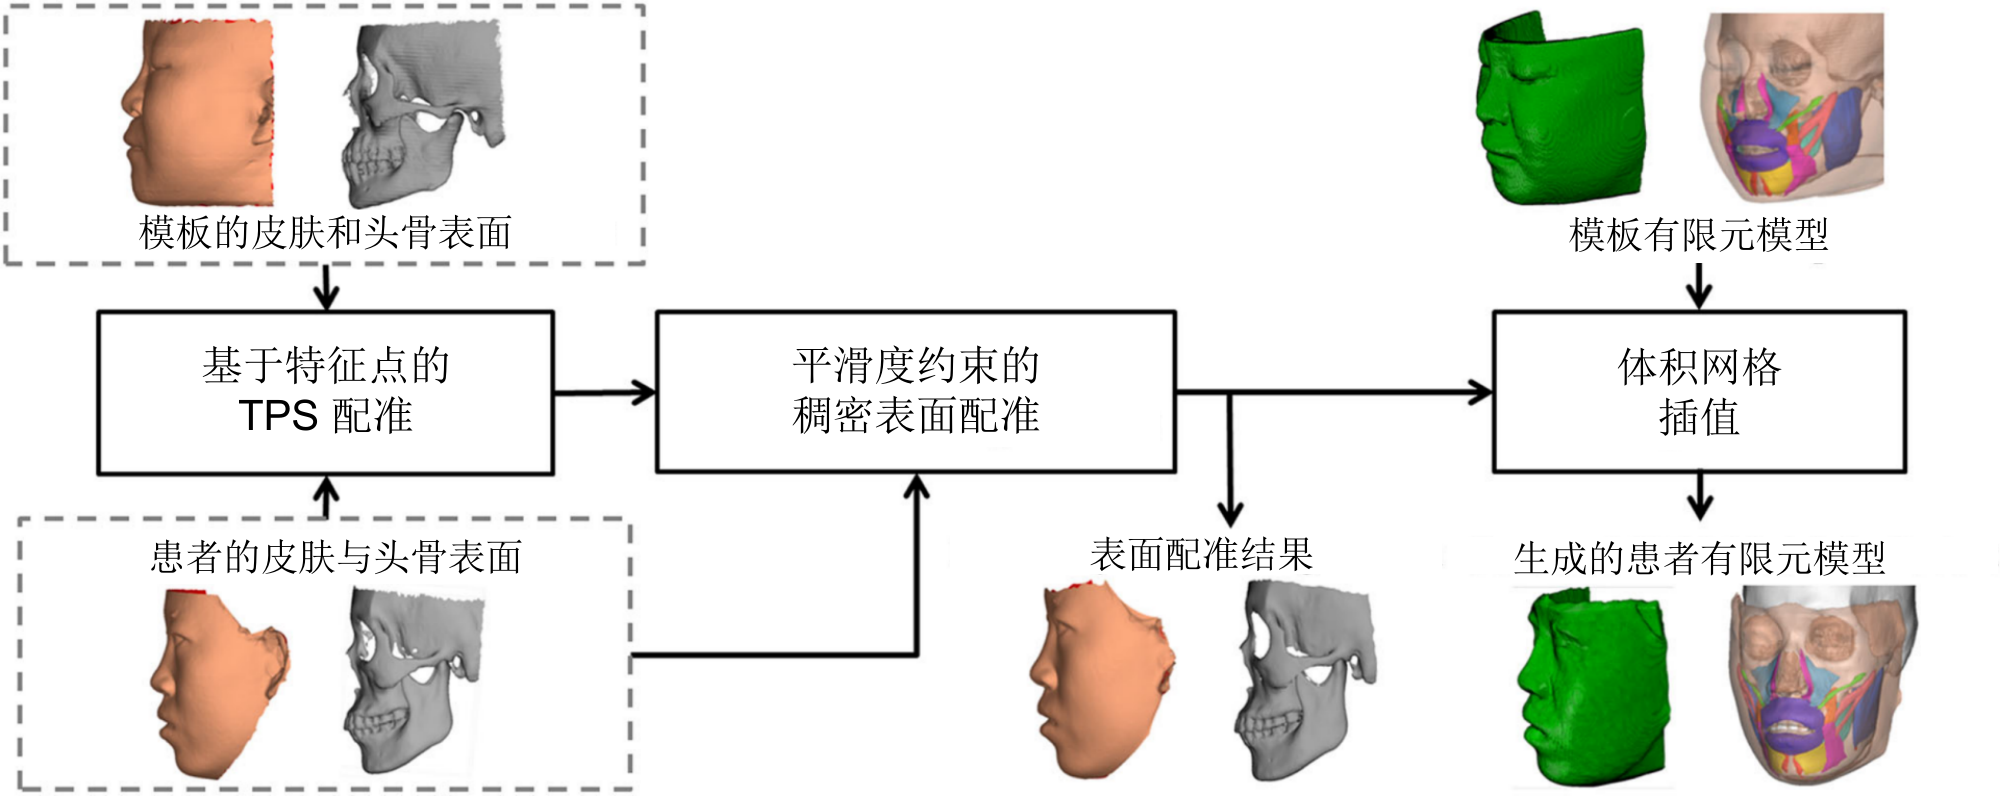
\includegraphics[width = \linewidth]{related-work/zhangEFacetemplateMethodEfficiently2016-cn.png}
  \caption{eFace-Template 技术框架 \cite{zhangEFacetemplateMethodEfficiently2016}}
  \label{fig:zhangEFacetemplateMethodEfficiently2016}
\end{figure}

\section{整形手术模拟研究进展}

在整形手术模拟领域,学术界已经进行了广泛而深入的研究。
目前,研究工作大致可以归结为两个主要方向:一是基于数据驱动的方法,这类方法使用先进的数据处理技术,以便预测整形手术的效果;另一方向是基于生物力学原理的仿真技术,该类技术利用计算机模型来精确预测手术后的结果。

\subsection{数据驱动的方法}

在计算机视觉的研究领域中,Zesong Qiu 等研究员 \cite{qiuSCULPTORSkeletonconsistentFace2022a} 提出了一个颇具创新性的三维参数化面部模型,被称为 SCULPTOR,其独特之处在于模型能够表达人类的骨骼结构。SCULPTOR 模型以 LUCY 数据集作为基础,将面部模型按不同维度进行解构,这些维度包括形状、姿态、表情等,从而构建了一种混合形状的表达形式。
该模型的核心在于以参数化方法驱动,集成了人类头骨结构、面部几何形状的建模,能够精确地捕获面部特征以及其背后的骨架结构。
特别是模型中引入的 trait 分量,对于模拟骨骼结构变化所引起的面部特征改变至关重要,这对于精确预测正颌手术患者术后面部外观的变化具有非常关键的意义。

\begin{figure}
  \centering
  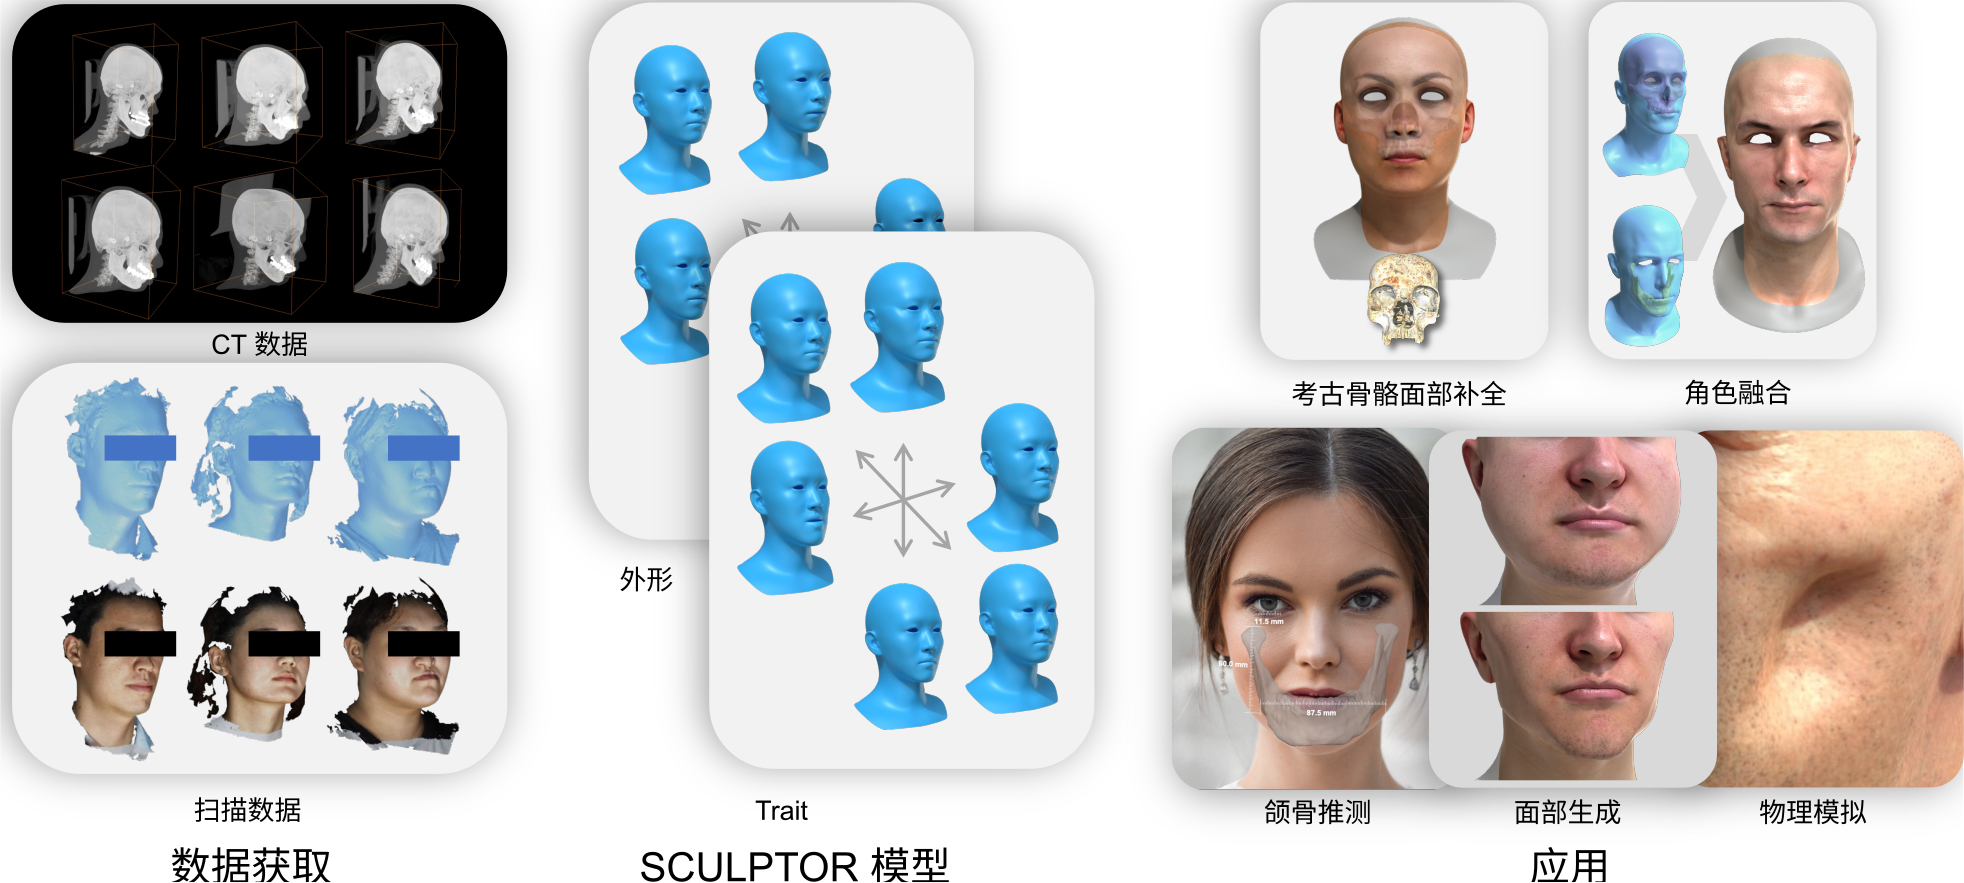
\includegraphics[width = \linewidth]{related-work/qiuSCULPTORSkeletonconsistentFace2022a-cn.png}
  \caption{SCULPTOR 模型概览 \cite{qiuSCULPTORSkeletonconsistentFace2022a}}
  \label{fig:qiuSCULPTORSkeletonconsistentFace2022a}
\end{figure}

在计算机视觉的研究领域内,深度学习技术已经取得了令人瞩目的成就,尤其在图像分类、目标检测和语义分割等任务上有卓越的表现。
近年来,众多研究者也开始探索将此技术应用于手术模拟的可能性。
Ma Lei 等研究人员 \cite{maSimulationPostoperativeFacial2023} 开发出一种称为 FSC-Net 的新型面部模型预测网络。
FSC-Net 的框架如图 \ref{fig:maBidirectionalPredictionFacial2023} 所示,该网络旨在学习从骨骼形态变化到面部外形变化之间的复杂且非线性的关系。
值得注意的是,FSC-Net 基于点变换网络结构,采用术前后成对数据进行弱监督学习来优化网络参数,这一过程无需严格的顶点对应匹配。
同时,为了提高建模的准确性,尤其是下颌部位,网络采用了以距离为基础的形状损失函数。
为了保持网格顶点的一致性并避免尖锐或不切实际的变形,FSC-Net 对顶点位移进行约束,以计算局部顶点损失。
实验评估显示,FSC-Net 在处理速度上比传统的有限元方法提高了 15 倍,同时还保持了与有限元方法相近的精度。

\begin{figure}
  \centering
  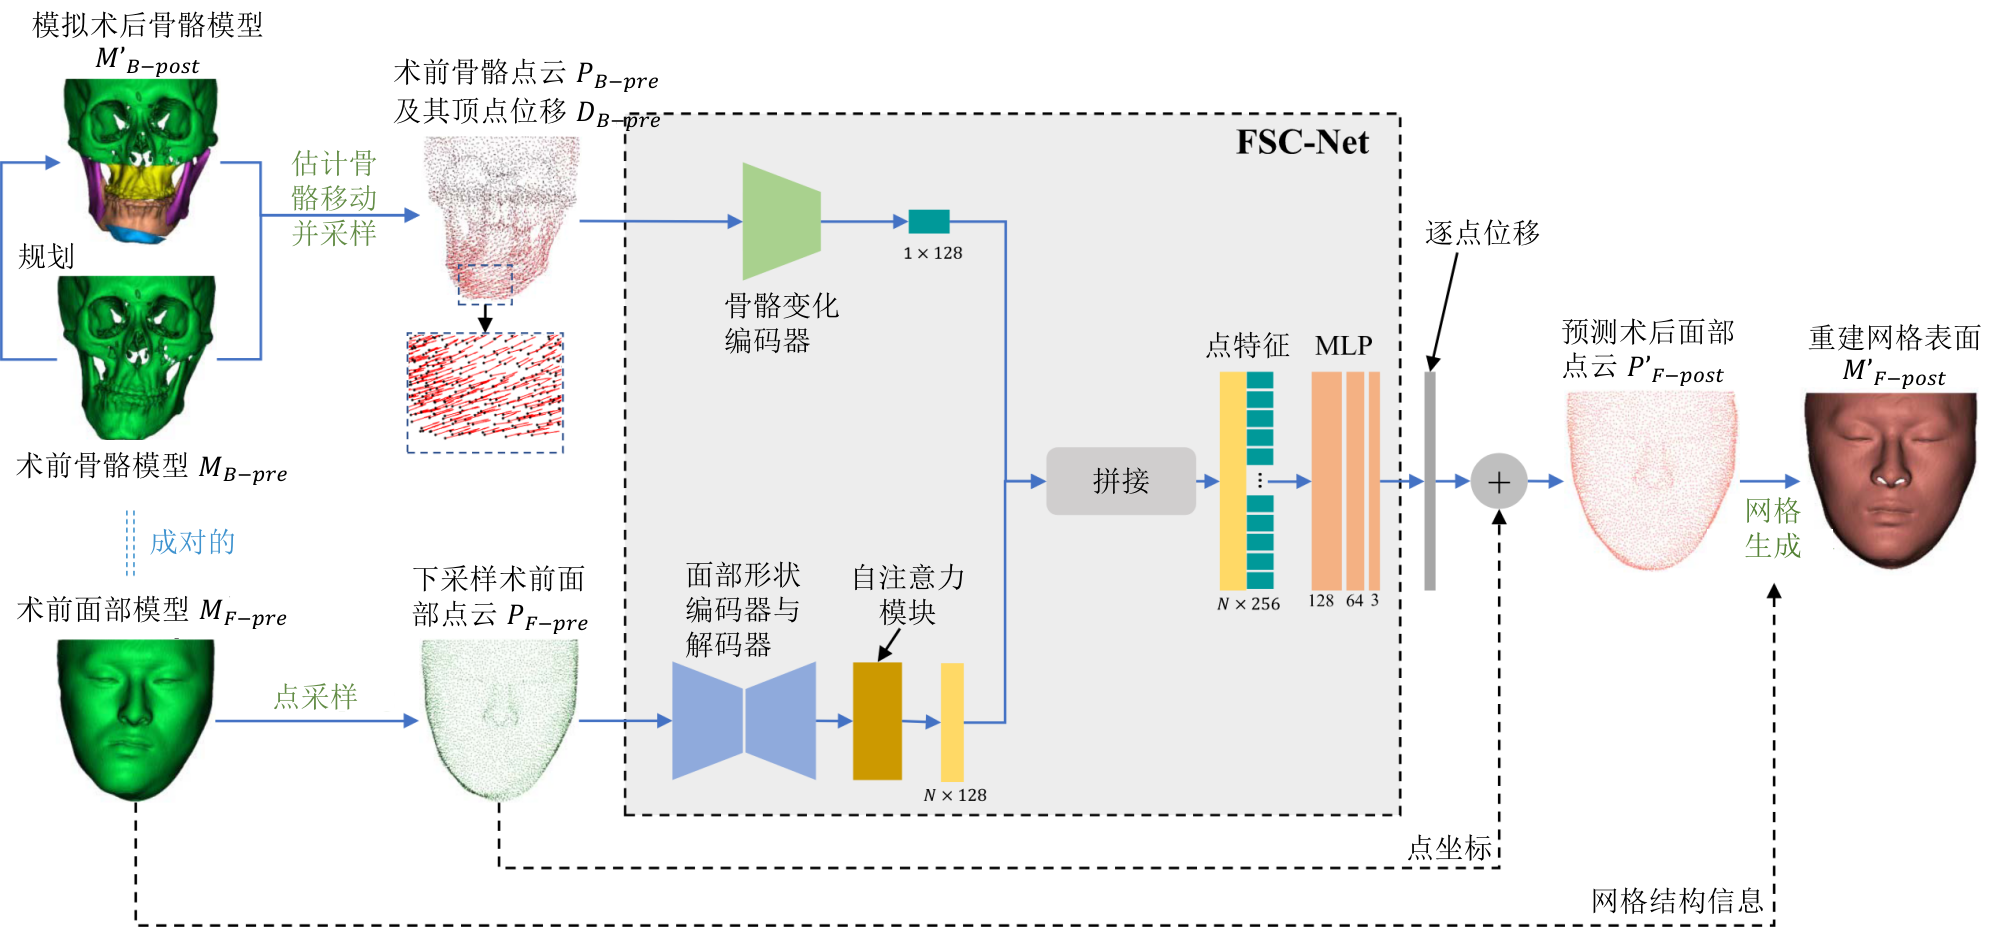
\includegraphics[width = \linewidth]{related-work/maSimulationPostoperativeFacial2023-cn.png}
  \caption{
    FSC-Net 框架概述 \cite{maBidirectionalPredictionFacial2023}
    % 。N:降采样后术前面部点云中的点数。MLP:多层感知器。
  }
  \label{fig:maBidirectionalPredictionFacial2023}
\end{figure}

在近一步的研究中,Ma Lei 等学者 \cite{maBidirectionalPredictionFacial2023} 在 P2P-Net \cite{yinP2PNETBidirectionalPoint2018} 的基础上进行了扩展,开发了一种新型深度学习模型,称为双向点对点卷积网络(P2P-Conv)。
这一模型专为解决面部和颅骨之间形态转换的问题而设计,旨在协助正颌外科手术规划。
P2P-Conv 不仅保留了 P2P-Net 的优势,还整合了动态点卷积(PointConv)技术,有效地提取了局部和全局空间信息。
模型训练时,该框架采用了多子集数据增广技术,通过分割面部和颅骨顶点为多个子集数据来增强训练过程。
在推理阶段,结合多子集产生的结果,可得到一致且精确的密集顶点变换预测。
实验结果表明,P2P-Conv 在面部和颅骨形态互换的预测准确性上取得了显著的进步。
然而,目前的方法还未能充分考虑到人体个体特异性这一问题 --- 例如,即便是颅骨形状极其相似的不同个体,他们的面部形态也可能存在显著的差异。

\subsection{物理仿真方法的研究进展}

关于面部软组织计算建模技术的研究已经吸引了广泛的关注,并取得了一系列深入的成果。
根据使用的建模方法不同,这些研究大致可以分为三大类:质点-弹簧模型(Mass Spring Model,MSM)、有限元模型(Finite Element Model,FEM)及质点-张量模型(Mass Tensor Model,MTM)。

在这三种模型中,由于计算效率上的显著优势,MSM 常被应用于实时面部动画制作。
Terzopoulos \cite{terzopoulosPhysicallyBasedFacial1990} 以及 Lee \cite{leeRealisticModelingFacial1995} 在该领域起到了开拓性的作用,他们开发的基于线性弹性肌肉的 MSM 能够高效地模拟面部动画。
此外,Keeve 等研究者 \cite{keeveDeformableModelingFacial1998} 提出了采用棱柱单元的 MSM,并针对精确度与计算成本,与有限元方法(FEM)进行了比较分析。

经过深入研究,Teschner 等学者 \cite{teschnerDirectComputationNonlinear} 提出了一种改进的多层非线性 MSM,该方法通过引入静态约束来直接计算面部模拟仿真中的平衡状态。
Vicente \cite{vicenteMaxillofacialSurgerySimulation2009} 的工作专注于利用 MSM 技术模拟面部手术后的形态变化,创新性地设计了基于六面体元素网格的 MSM。
这个模型在理论上与传统线性 FEM 等价,并通过位移尺度调整技术细致模拟软组织的物理响应。

与传统的 MSM 对比,FEM 在模拟生物力学特性方面具有更高准确性,尽管其计算相对更加耗时。
Kim 等研究者 \cite{kimClinicallyValidatedPrediction2017} 提出了一种新颖的三阶段有限元方法,通过模拟组织之间的滑动来增强面部软组织变形预测的精确度。
在第一阶段,该方法利用 eFace-Template \cite{zhangEFacetemplateMethodEfficiently2016} 构造患者的网格模型,并以手术后骨骼的位移作为边界条件,应用 FEM 模拟软组织响应。
第二阶段引入节点力约束来仿真软组织与骨骼之间的滑动效应,显著提升了模拟结果的质量。
最后,在第三阶段通过重构软组织与骨骼间的映射关系,并引入新的节点间空间约束作为边界条件,进一步增强模拟组织滑移效应的仿真质量。
研究表明,这种改良的 FEM 在模拟面部结构,特别是在临床关键区域如鼻子和口唇的精确度方面,相较于现有的其他 FEM 技术有明显提高。

为了精确预测面部软组织术后的位置变化,Knoops等研究者 \cite{knoopsNovelSoftTissue2018} 开发了创新的概率有限元模型。
该模型结合了实验设计方法(Design Of Experiments,DOE)与迭代优化策略,成功地生成了一系列具有概率预测区间的三维面部模型,特别是针对鼻部和上唇区域,展现出高度的预测准确性。
此项研究深入剖析了模型的不准确性和手术计划执行中的不确定性对软组织预测结果的影响。
此外,该模型为手术规划提供了可能的区间预测,对于帮助患者充分了解手术可能引起的面部变化具有重要的临床意义。

在数值模拟领域,MTM 的设计宗旨是实现计算效率与结果精度之间的优化平衡。
开拓性研究者 Cotin 等人 \cite{cotinHybridElasticModel2000} 率先提出了一种基于 MTM 的混合弹性模型,该模型致力于精确描绘软组织在局部变形时表现出的复杂物理效应。
在此基础上,Picinbono 及其研究伙伴 \cite{picinbonoNonlinearAnisotropicElasticity2003} 进一步发展了这一模型,将其应用到非线性各向异性材料的相关研究中。

Mollemans 的研究团队 \cite{mollemansPredictingSoftTissue2007} 创新性地将 MTM 技术应用于颅颌面手术的软组织模拟中,通过对临床案例的定量与定性评估,首次实地验证了该技术在此类应用中的可靠性和有效性。
此后,Kim 等研究者 \cite{kimNewSofttissueSimulation2010} 使用了横向各向同性的 MTM,探索如何进行面部软组织行为的预测,并提出了一种同时满足生物力学原理与高效率仿真需求的软组织模拟方法。

在类似研究的进一步深化中,Ichim 及其同事 \cite{ichimPhacePhysicsbasedFace2017} 创新性地提出了 Phace --- 这是一种基于物理原理的面部动画技术。
Phace 建立在一个精心构建的通用面部模板之上,如图 \ref{fig:ichimPhacePhysicsbasedFace2017} 所示,其中包含了组织和骨骼的体积表示、嵌入四面体网格的肌肉模型、一组混合形状基等信息。
与传统的模拟方法不同,Phace 通过最小化被动肌肉、主动肌肉与骨骼这些刚体结构交互作用过程中的势能,实现对于面部表情动态变化的精确计算。
而且,Phace 通过将碰撞处理机制与仿真模型整合,有效规避了传统动画技术如混合形状建模中常见的穿模问题。
通过引入的全新肌肉激活模型,Phace 能够有效地复现复杂的面部表情。
Phace 所展现出的应用潜力极为广泛,它不仅适合于艺术动画制作的场景,还可服务于模拟整形手术过程中的面部重塑以及脸部与外力或物体相互作用的动态模拟。

\begin{figure}
  \centering
  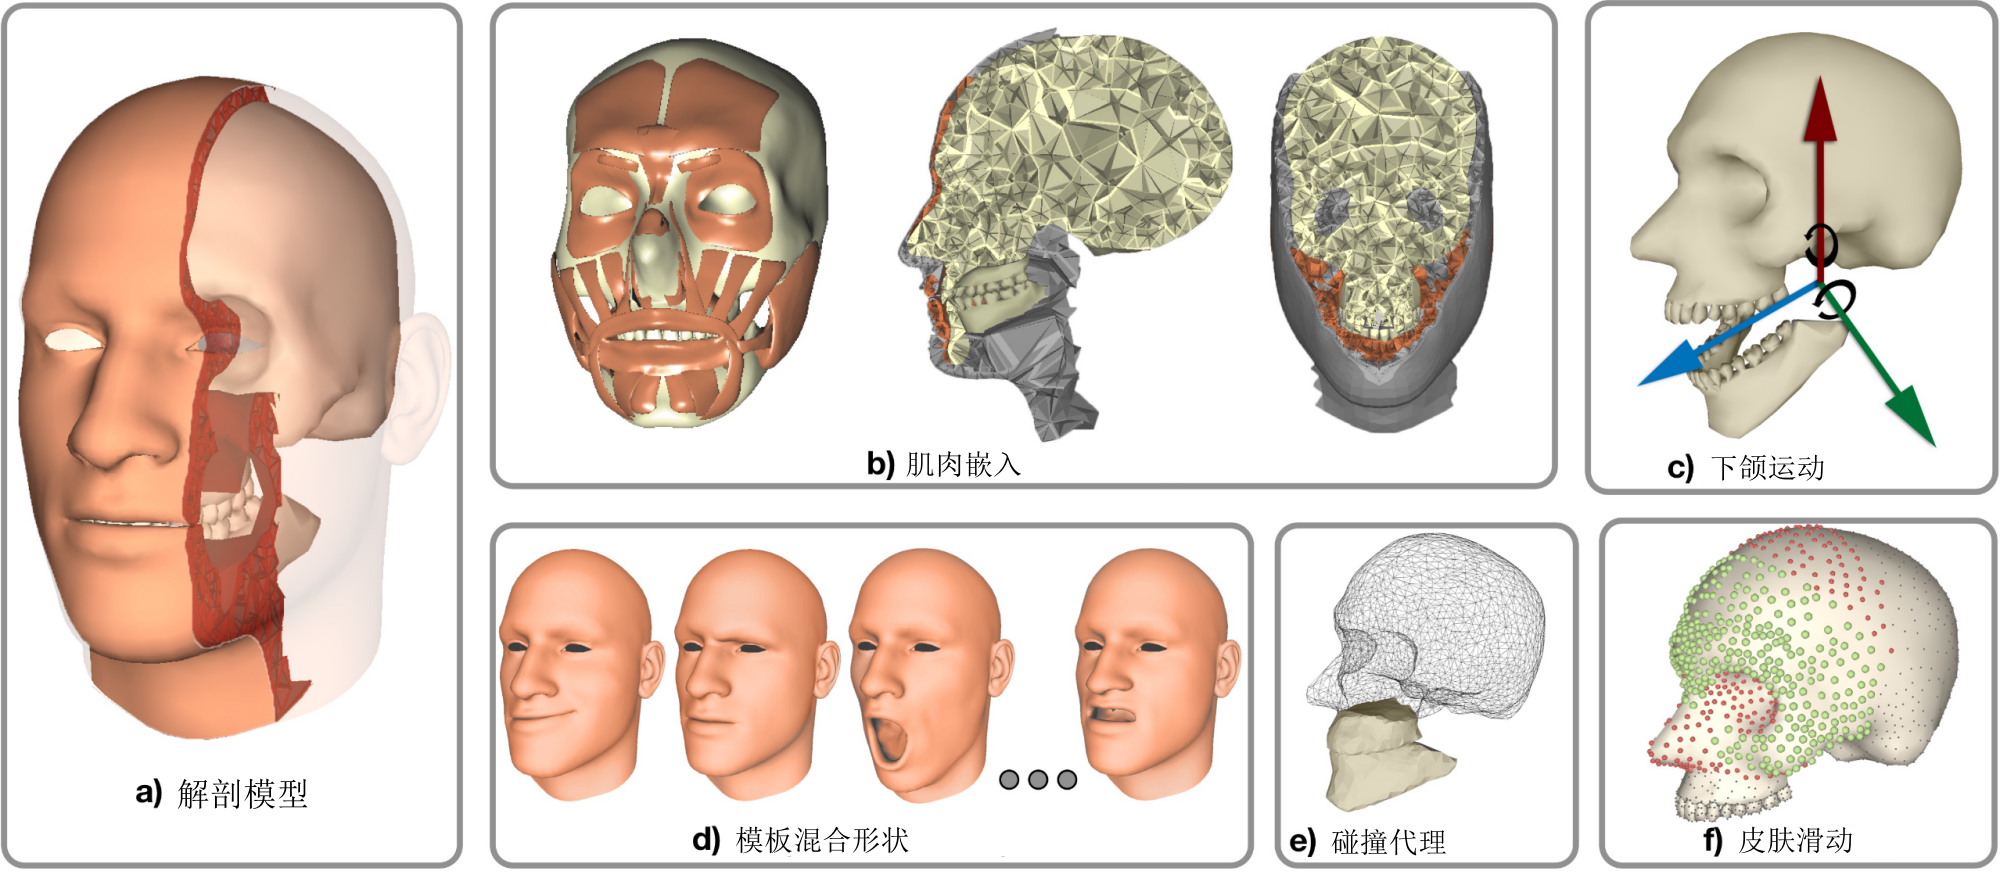
\includegraphics[width = \linewidth]{related-work/ichimPhacePhysicsbasedFace2017-cn.png}
  \caption{Phace 模板构成 \cite{ichimPhacePhysicsbasedFace2017}}
  \label{fig:ichimPhacePhysicsbasedFace2017}
\end{figure}

% % !TeX root = ../thuthesis-example.tex

\chapter{三维面部和骨骼模型的重建}
\label{cha:reconstruction}

精确和高效的正颌外科手术模拟,其先决条件是从医疗成像数据中准确重建出三维的面部与骨骼模型。
为了获得手术前后骨骼的变化,我们需要获得手术前后骨骼顶点的一一对应关系。
因此,我们还需要将模板模型与患者模型进行配准以获得手术前后同拓扑的网格模型。
本章详尽地阐述了该三维模型重建的方法和流程,具体内容包括:
\begin{enumerate}
  \item 提取 CT 图像数据以形成面部与骨骼表面模型的三角网格表示,
  \item 对模板模型与患者模型进行刚性配准,
  \item 采用非刚性配准对模板模型进行形变,以更精确地匹配骨骼和表面的形状,
  \item 对模型表面进行体积细分,以构建模拟患者软组织的四面体网格。
\end{enumerate}
经过以上步骤,我们能够生成手术前后拓扑基本一致的三角网格模型,并且将该模型划分为高质量的四面体网格。

本文所采用的 CT 数据分辨率为 \numproduct{512 x 512 x 364} 体素,每个体素的尺寸为 \qtyproduct{0.4395 x 0.4395 x 0.6000}{\milli\meter}。

\section{模板模型的构建}

为满足本研究的需求,我们以 SCULPTOR \cite{qiuSCULPTORSkeletonconsistentFace2022a} 开源的骨骼及面部模板为基础,构筑了所需的模板模型。
初始阶段,我们手动移除 SCULPTOR 模板中的非必要部分,如颈部和复杂的口唇区域。
随后,利用 MeshFix 工具 \cite{atteneLightweightApproachRepairing2010} 填补了模板中的空洞,这些空洞主要位于眼部、口部以及颈部的精细区域,并解决了因自相交缺陷导致的穿模问题。
最后,我们对模型应用了 Taubin 平滑 \cite{vollmerImprovedLaplacianSmoothing1999},以降低模型中的锐利缺陷。

\section{刚性配准}

本节主要讲述如何从 CT 体素数据提取三角网格表面模型,并进行模型之间的刚性配准。

首先,我们对体素数据施加 Gaussian 平滑处理,以滤除 CT 扫描中由散射和噪声所引入的过锐缺陷。
之后,按照预设阈值对 CT 值进行分割,并使用 VTK Contour Filter 方法提取骨骼和面部的等值面,其中骨骼和软组织的 CT 阈值分别设置为 \num{200} 和 \num{-200}。

进一步,在模板和患者的三维模型的骨骼表面上分别标定了若干特征点,如图 \ref{fig:landmarks} 所展示的 10 个和 9 个特征点。
该步骤的目标是在模板与患者间建立精确的一对一特征点映射关系。

\begin{figure}
  \centering
  \subcaptionbox{10 个面部特征点\label{fig:landmarks-face}}{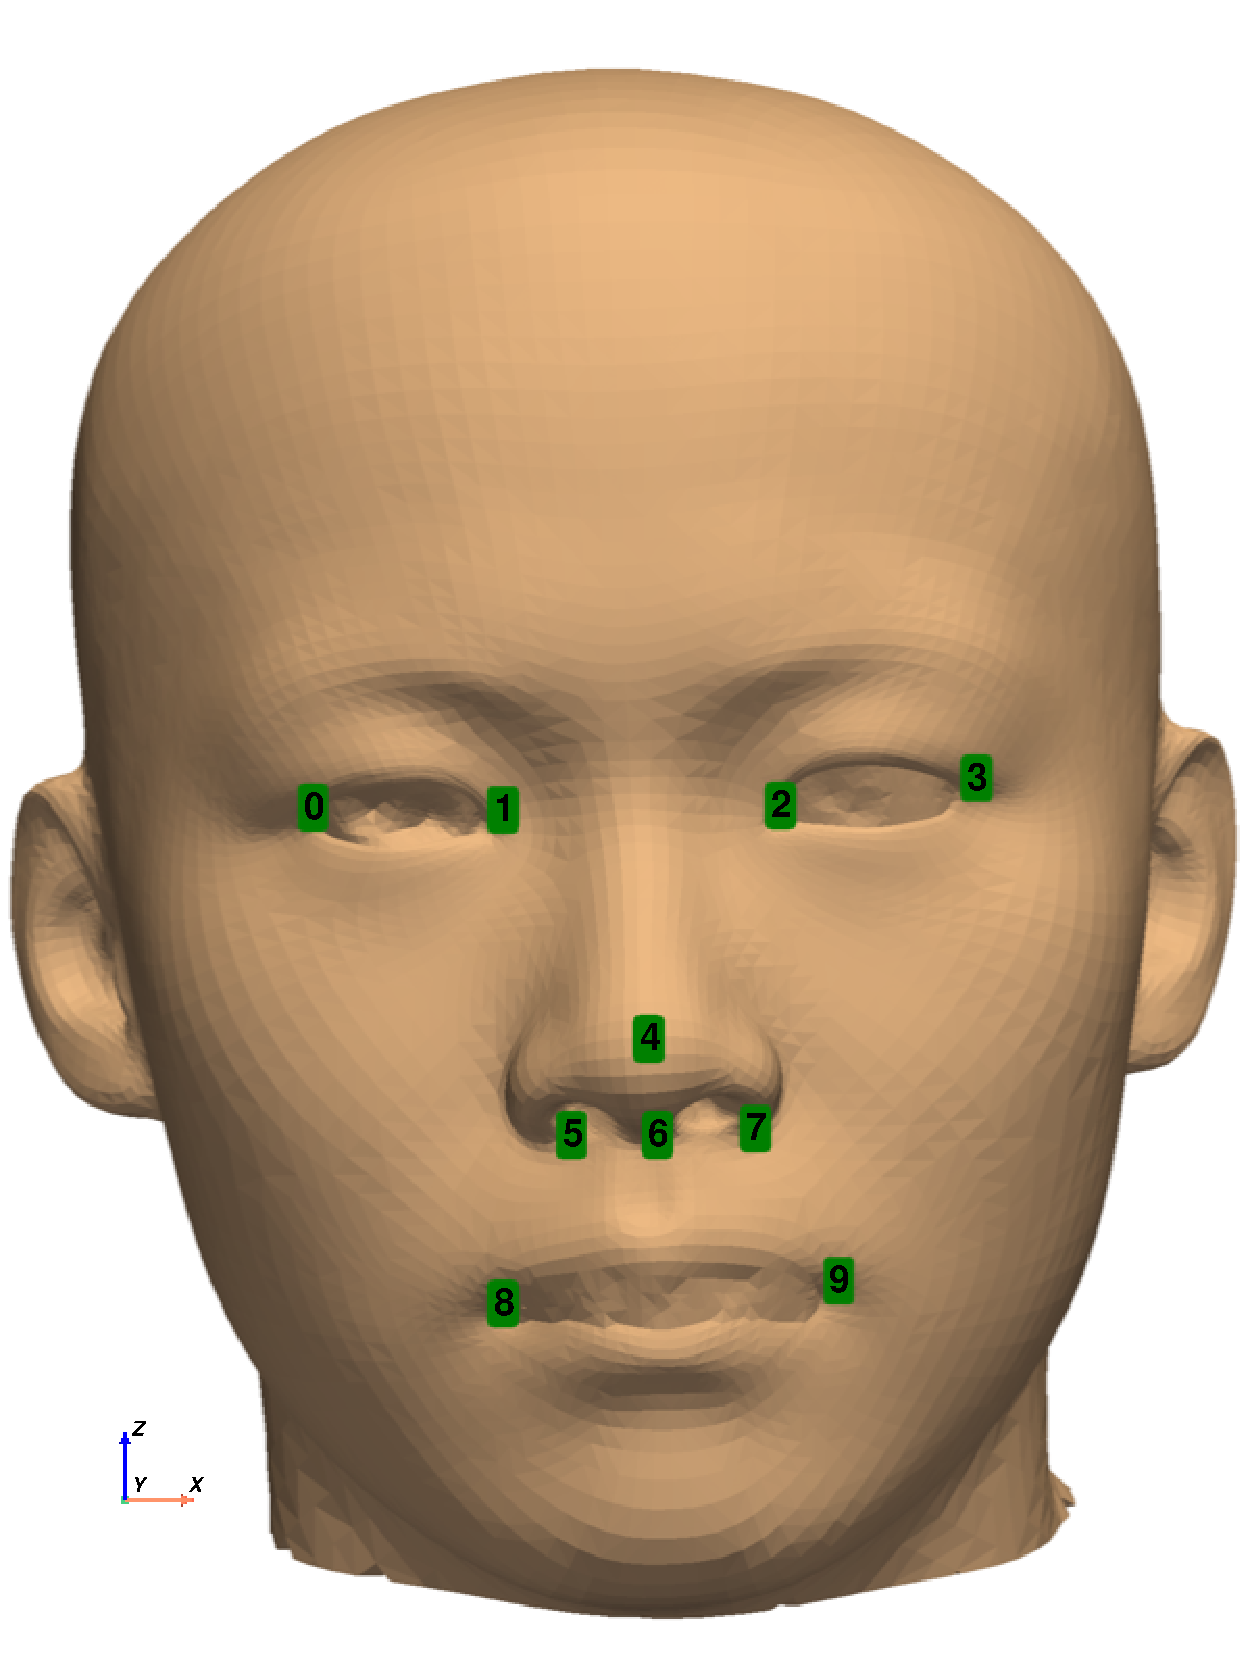
\includegraphics[width = 0.3 \linewidth]{landmarks/face-landmarks.pdf}}
  \subcaptionbox{9 个骨骼特征点\label{fig:landmarks-skull}}{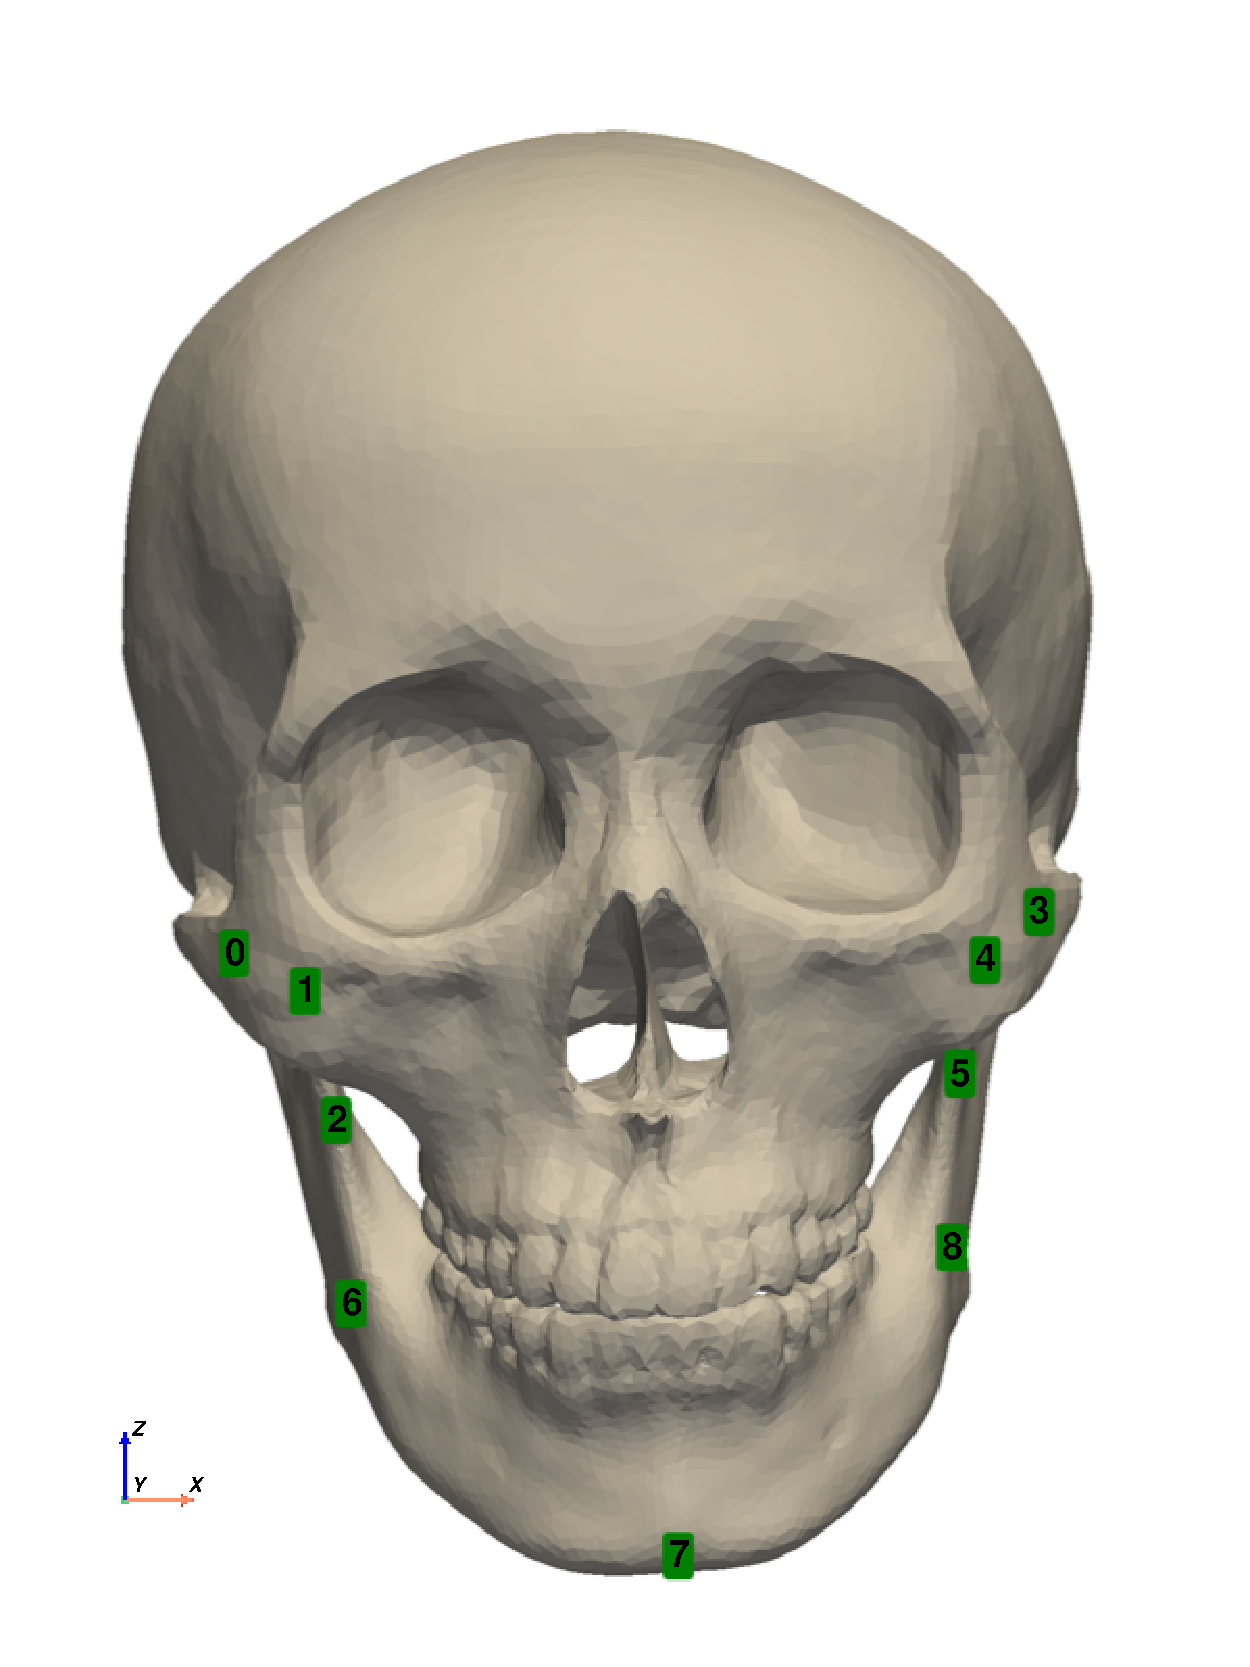
\includegraphics[width = 0.3 \linewidth]{landmarks/skull-landmarks.pdf}}
  \caption{特征点}
  \label{fig:landmarks}
\end{figure}

为了获得一组初始的刚性变换参数,即全局的平移、缩放与旋转参数,本研究采纳了标准的 Procrustes 分析方法 \cite{rossProcrustesAnalysis2004}。
Procrustes 分析的核心目标在于通过反复迭代的过程,最小化两组特征点之间的总平方距离。
在此基础之上,本研究进一步引入了迭代最近点(Iterative Closest Point,ICP)算法,对模型进行精细的刚性配准。
该步骤的主要目的在于减小由人工标注特征点过程中可能产生的误差。
具体的刚性配准结果如图 \ref{fig:align} 所展示。
值得注意的是,CT 数据往往具有相近的空间位态,因此对于多组 CT 扫描,我们可以通过单次 Procrustes 分析为所有模型建立一个相同的初始变换参数,再通过 ICP 算法进行进一步的提升配准的精度。

\begin{figure}
  \centering
  \subcaptionbox{面部}{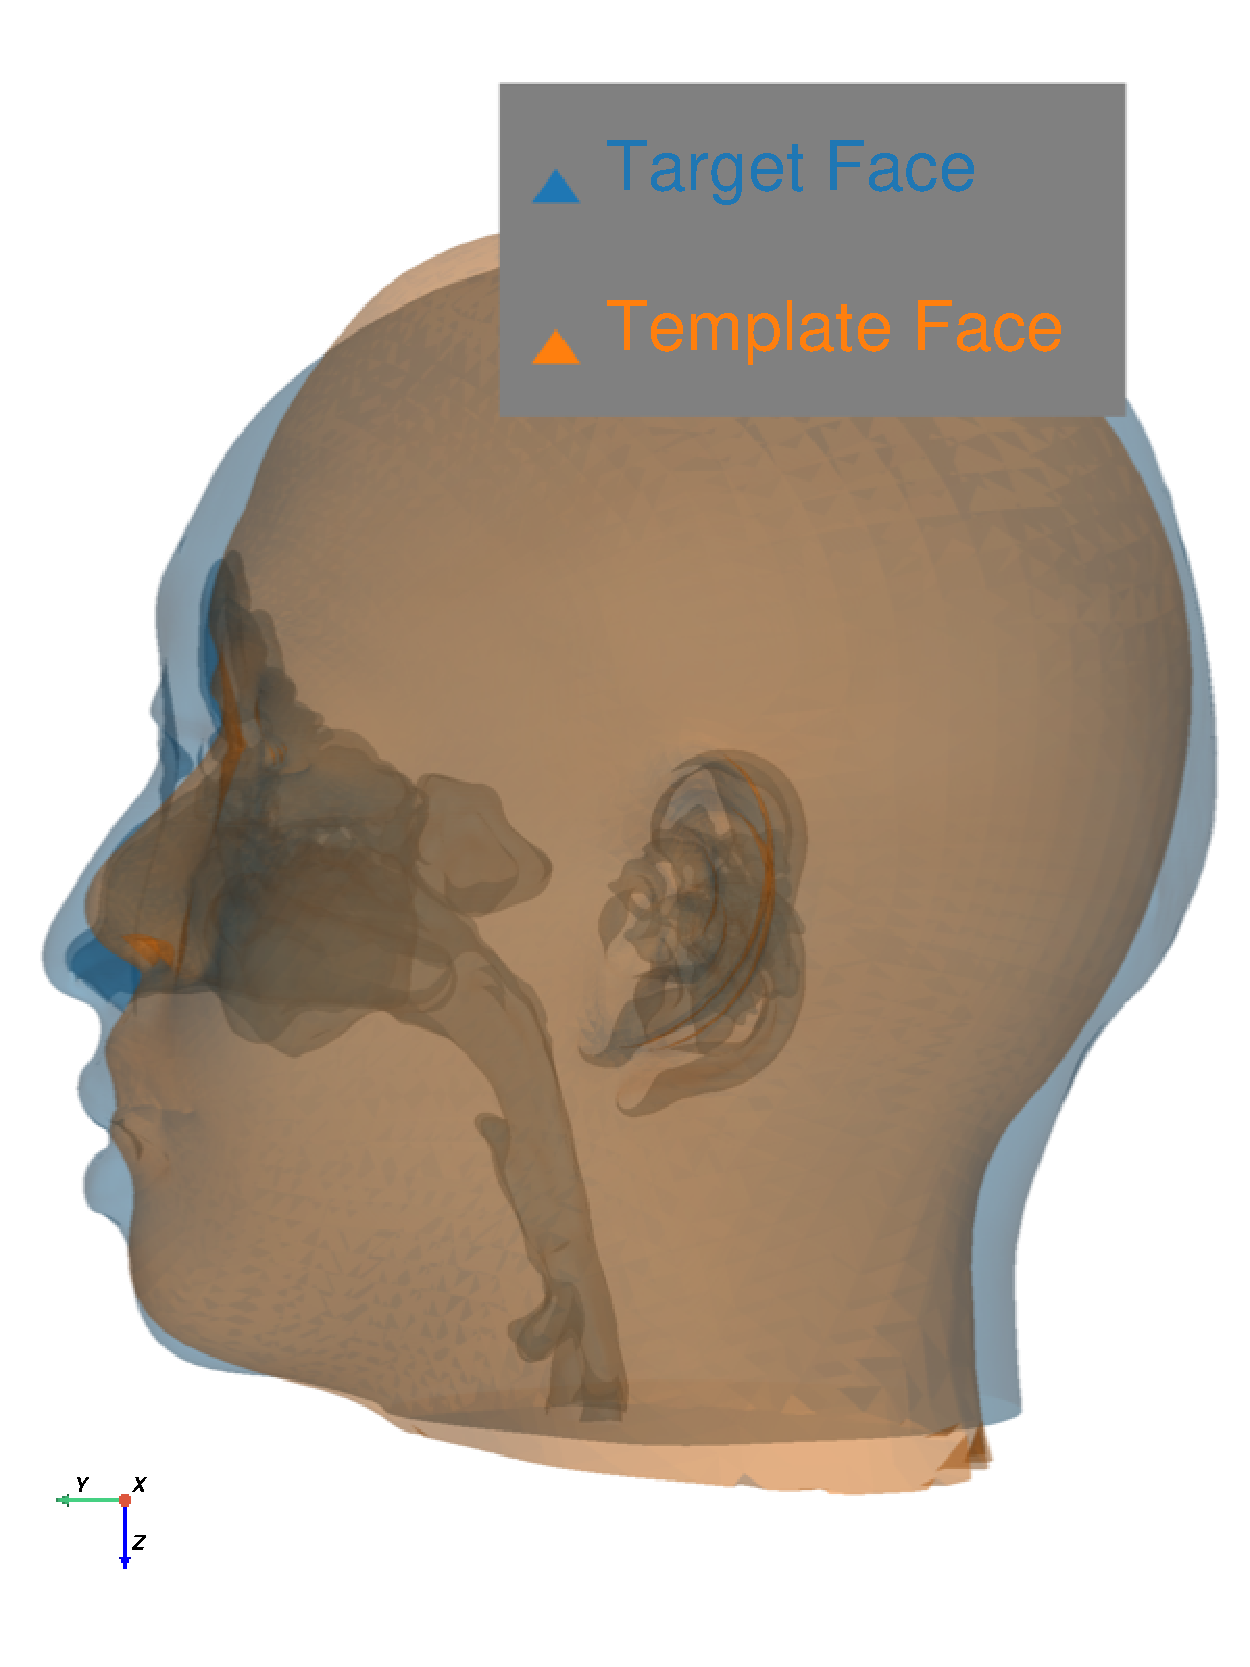
\includegraphics[width = 0.3 \linewidth]{align/align-face.pdf}}
  \subcaptionbox{骨骼}{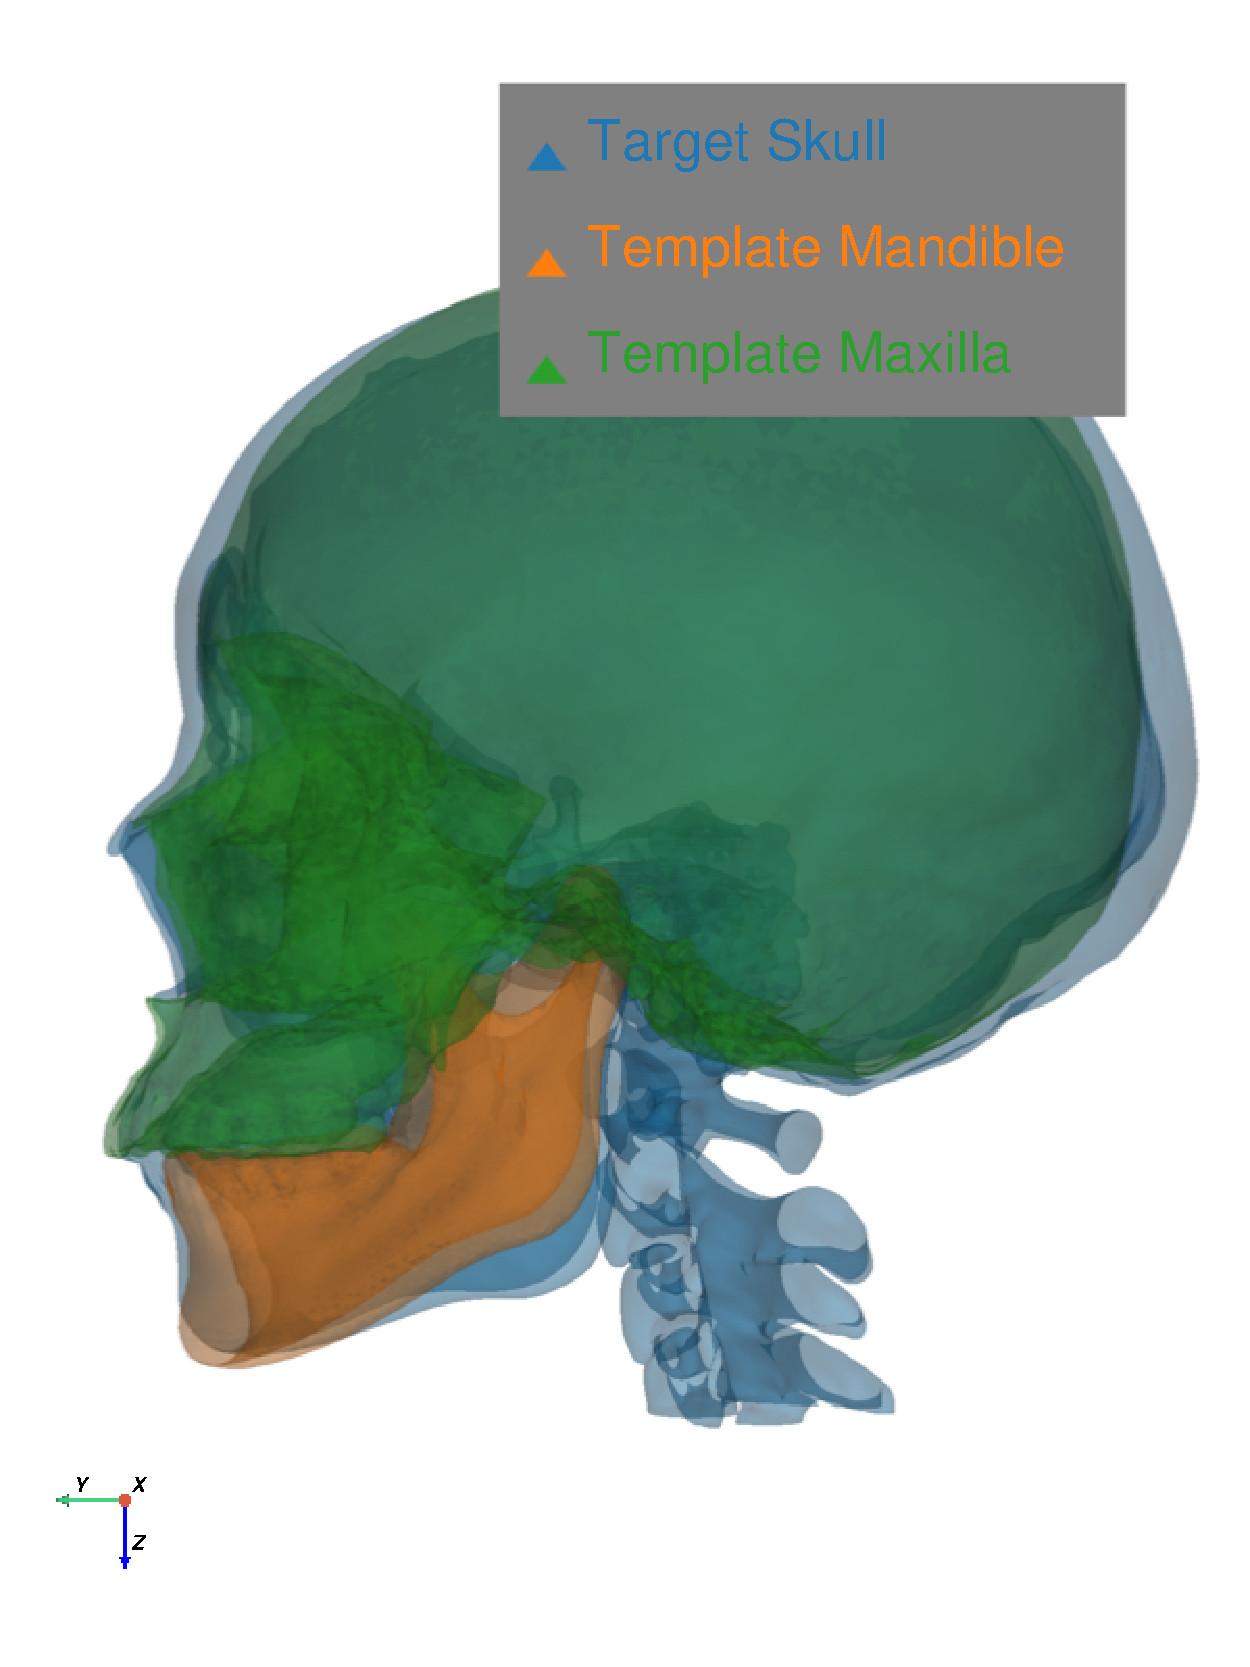
\includegraphics[width = 0.3 \linewidth]{align/align-skull.pdf}}
  \caption{刚性配准结果}
  \label{fig:align}
\end{figure}

\section{非刚性配准}

在完成了初始的刚性配准工作后,我们需要进行非刚性配准(non-rigid registration),以将模板模型变形至与患者一致。
我们采用了由 Amberg 等人提出的非刚性配准算法 \cite{ambergOptimalStepNonrigid2007} 作为理基础。
该算法将 ICP 扩展至非刚性形变来使模型与目标几何匹配。
在初始阶段,通过使用最邻近点来建立模板与目标患者模型间顶点的对应关系。
继而,该算法通过最小化能量函数 $E$ 来解算每个顶点的变换矩阵 $\bm{X}_i$。
在迭代过程中,对应关系与变换矩阵的交替进行更新,随着迭代次数的增加,对应关系趋于更为精确,引导变换矩阵的优化结果逐渐接近理想状态。

\subsection{对应关系的建立}

在考虑模板与患者模型之间的区域差异,例如,患者模型的面部部分相比模板多出口腔等区域,而其骨骼结构又包括额外的脊椎但不包含牙齿咬合面等细节。
由此,我们必须从两者中抽取交集区域,亦即重叠区域。
首先,我们对模板进行标注,标记出重叠区域 $\mathcal{S}_o$。
接着,可以根据下式确定患者模型的重叠区域 $\mathcal{T}_o$:
\begin{equation}
  \mathcal{T}_o = \Bqty{\bm{u}_i \mid \dist(\mathcal{S}_o, \bm{u}_i) < \tau, \bm{u}_i \in \mathcal{T}}
\end{equation}
其中,$\tau$ 代表预设的阈值。
在实际操作中,我们将 $\tau$ 设为对应患者模型边界框的对角线长度的 \SI{5}{\percent}。
从同一成像设备获取的 CT 数据中,重叠区域在空间范围上具有相似性。
因此,处理多组数据时,仅需对模板的重叠区域进行一次标注,再将该标注信息应用于其他患者模型即可。
这大大节省了时间和人力资源。

简单地采用最近邻顶点法进行初始化对应关系可能导致模板与患者模型之间的对齐不够精确。
例如,在下颌骨较为扁平的区域,最近邻顶点法可能会受限于狭窄空间,使得无法有效地将模板中的顶点与患者模型中的顶点匹配起来。
为了克服这一限制,在初始化对应关系时,我们加入了顶点法线作为额外的依据变量:
\begin{equation}
  \mathrm{NN}(\bm{v}_i) = \argmin_{\bm{u}_j \in \mathcal{T}_o} \norm{\bm{v}_i - \bm{u}_j}^2 + \nu \norm{\bm{n}_i - \bm{n}_j}^2
\end{equation}
式中,$\mathrm{NN}(\bm{v}_i)$ 表示模板顶点 $\bm{v}_i$ 在患者模型中的最近邻对应点,$\bm{n}_i$ 和 $\bm{n}_j$ 分别为模板顶点 $\bm{v}_i$ 与患者模型对应顶点 $\bm{u}_j$ 的法向量,而 $\nu$ 是一个超参数,用于调整法线在匹配过程中的权重。
我们利用 $k$-d 树(其中 $k = 6$)加速最近邻关系的搜索过程,此算法使得我们能够以 $\mathcal{O}(n \log{m})$ 时间复杂度完成所有顶点对应关系的确定,其中 $n$ 表示模板顶点的数量,$m$ 表示患者模型顶点的数量。
这种方法同样适用于求解反向对应关系。

\subsection{损失函数}

我们考虑一个包含 $n$ 个顶点的模板,其顶点集定义为 $\mathcal{S} = \{\bm{v}_i\}$,并且在模板上规定了一个重叠区域 $\mathcal{S}_o$。
我们的目标是识别一种逐顶点变换 $\mathcal{X}$,以便使得模板的重叠区域 $\mathcal{S}_o$ 能够适当变形以匹配到患者模型 $\mathcal{T}_o$ 上。
因此,我们将每个顶点的变换建模为一个包含平移和相对于模型中心旋转,数学上表达为:
\begin{equation}
  \bm{v}_i' = \bm{X}_i \bm{v}_i
\end{equation}
这里,$\bm{X}_i \in \mathbb{R}^{3 \times 4}$ 表征了第 $i$ 个顶点所受的仿射变换矩阵,$\bm{v}_i = [x_i ~ y_i ~ z_i ~ 1]^T$ 则表示顶点的齐次坐标。

为了高效衡量模板与患者模型间的误差,我们采用了一个混合损失函数,该损失函数由距离项、刚度项和特征点项组成,用以作为模板与患者模型间差异的评估指标。

\paragraph{距离项}
该项的目的在于实现模板顶点向患者模型顶点的尽量准确对齐。
为达至此目标,我们定义了顶点距离损失函数如下:
\begin{equation}
  E_d(\mathcal{X}) = \sum_{\bm{v}_i \in \mathcal{S}_o} w_i \dist^2(\mathcal{T}_o, \bm{X}_i \bm{v}_i)
\end{equation}
其中,权重 $w_i$ 由模板顶点 $\bm{v}_i$ 的法向量 $\bm{n}_i$ 以及患者模型中对应顶点 $\bm{u}_j$ 的法向量 $\bm{n}_j$ 之间的点积所决定,即 $w_i = \bm{n}_i \cdot \bm{n}_j$。

\paragraph{刚度项}
在形变匹配的同时保持模板的原有刚性特性是极其重要的。
鉴于此,我们引入刚度项 $E_s$ 来度量此种特性。
刚度项的定义如下:
\begin{equation}
  E_s(\mathcal{X}) = \sum_{(\bm{v}_i, \bm{v}_j) \in \mathcal{E}} \norm{(\bm{X}_i - \bm{X}_j) \bm{G}}_F^2
\end{equation}
此处,$\mathcal{E}$ 代表模板中所有边的集合,而 $\bm{G} = \diag(1, 1, 1, \gamma)$ 是引进的权重矩阵,并且 $\norm{\cdot}_F$ 指的是 Frobenius 范数。
参数 $\gamma$ 用于对仿射变换的旋转部分与平移部分的权重进行平衡,本研究中 $\gamma$ 被设置为 1,以实现二者效应的均衡。

\paragraph{特征点项}
在优化模型的过程中,我们引入了特征点项 $E_l$,意在保障关键特征点对齐的精确性。
该项的定义如下式所示,简洁明了:
\begin{equation}
  E_l(\mathcal{X}) = \sum_{(\bm{v}_i, \bm{l}_i) \in \mathcal{L}} \dist^2(\bm{l}_i, \bm{X}_i \bm{v}_i)
\end{equation}
其中,$\mathcal{L}$ 代表人工标记的特征点对的集合。

通过对不同的损失函数组分施加权重,我们构建了最终权衡各项因素的优化目标函数,表示如下:
\begin{equation}
  E(\mathcal{X}) = E_d(\mathcal{X}) + \alpha E_s(\mathcal{X}) + \beta E_l(\mathcal{X})
\end{equation}
这里的超参数 $\alpha$ 与 $\beta$ 分别调节损失函数各组成部分的相对权重。

% 值得注意的是,我们的方法与 Amberg 等人提出的方法 \cite{ambergOptimalStepNonrigid2007} 存在区别。
% 为了保障配准结果能够满足后续仿真的质量要求,我们尤为注重避免自相交等瑕疵的产生。
% 损失函数中的 ``刚度项'' 在有效减小变形幅度的同时,也降低了穿模发生的风险。
% 特别地,我们提出了一种自动调节超参数 $\alpha$ 的策略,确保优化过程中模型始终避免自相交。
% 具体流程如下:
% \begin{enumerate}
%   \item 初始化 $\mathcal{X}$
%   \item 依次选用超参数 $\alpha^i \in \Bqty{\alpha^1,\dots,\alpha^n}$ (保证 $\alpha^i < \alpha^{i - 1}$)
%         \begin{enumerate}
%           \item 尝试 $\alpha_{cur} \in \Alpha(\alpha^i,\alpha^{i - 1})$
%                 \begin{enumerate}
%                   \item 使用插值法计算 $\alpha = \alpha_{cur}$ 时其他超参数的取值,例如 $\beta_{cur}$,$\nu_{cur}$
%                   \item 如果当前迭代的损失函数值 $E(\mathcal{X}) < \varepsilon$,则终止迭代
%                   \item 对损失函数 $E(\mathcal{X})$ 进行最小化处理,获得更新后的 $\mathcal{X}'$
%                   \item 检查更新后的网格 $\mathcal{X}' \mathcal{S}$ 是否存在自相交情况;若无,更新 $\mathcal{X} \leftarrow \mathcal{X}'$ 并进行下一 $\alpha^{i + 1}$ 的迭代
%                 \end{enumerate}
%         \end{enumerate}
% \end{enumerate}
% 其中,$\Alpha(\alpha^i,\alpha^{i - 1})$ 由以下等式定义:
% \begin{equation}
%   \Alpha(\alpha^i,\alpha^{i - 1}) = \Bqty{2^{-n} \alpha^i + (1 - 2^{-n}) \alpha^{i - 1} \mid n \in \mathcal{N}}
% \end{equation}

我们为非刚性配准精心设计了一组超参数,使得即便没有人工标注的特征点,我们的方法仍能够精准地将模板模型变形至与目标几何一致。
如图 \ref{fig:registration} 所示,非刚性配准的结果显示模板与患者模型之间几乎完美的重合,这为后续的仿真分析打下了坚实的基础。

\begin{figure}
  \centering
  \subcaptionbox{面部}{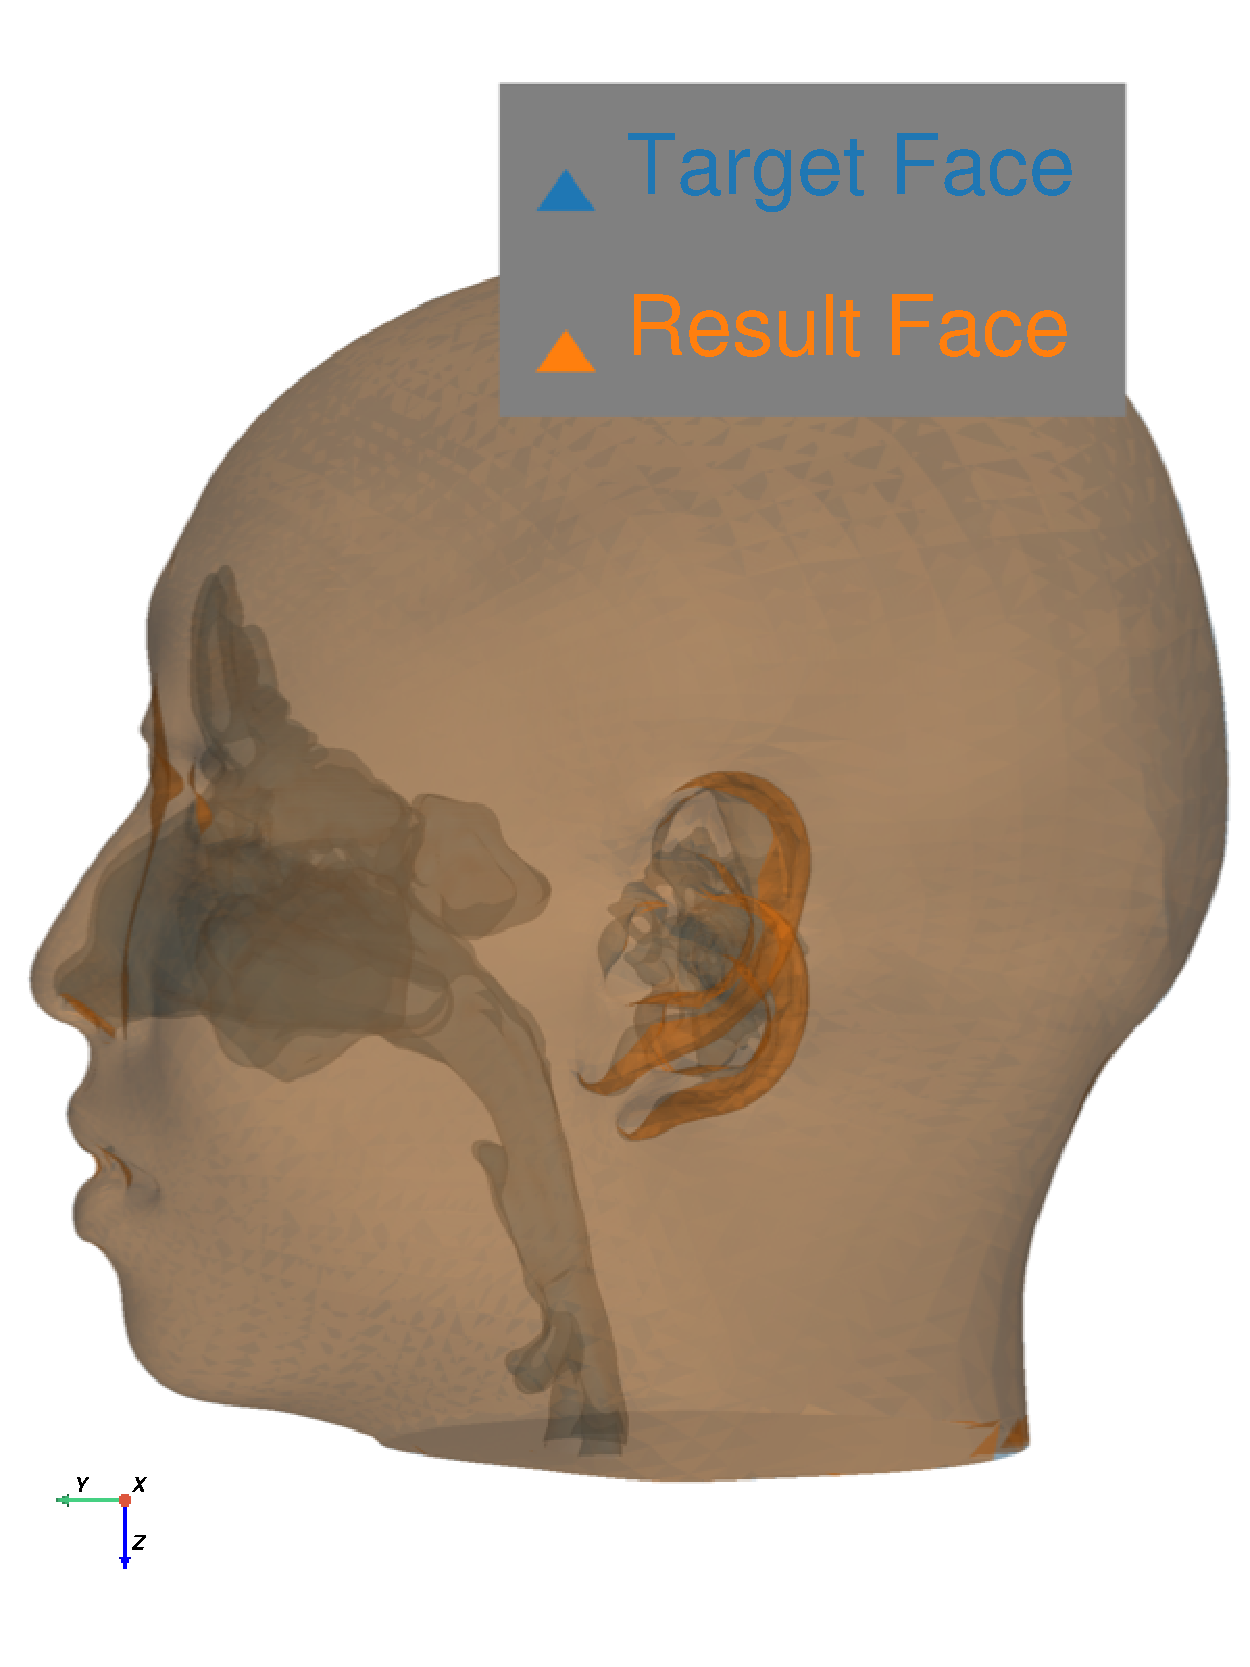
\includegraphics[width = 0.3 \linewidth]{register/register-face.pdf}}
  \subcaptionbox{骨骼}{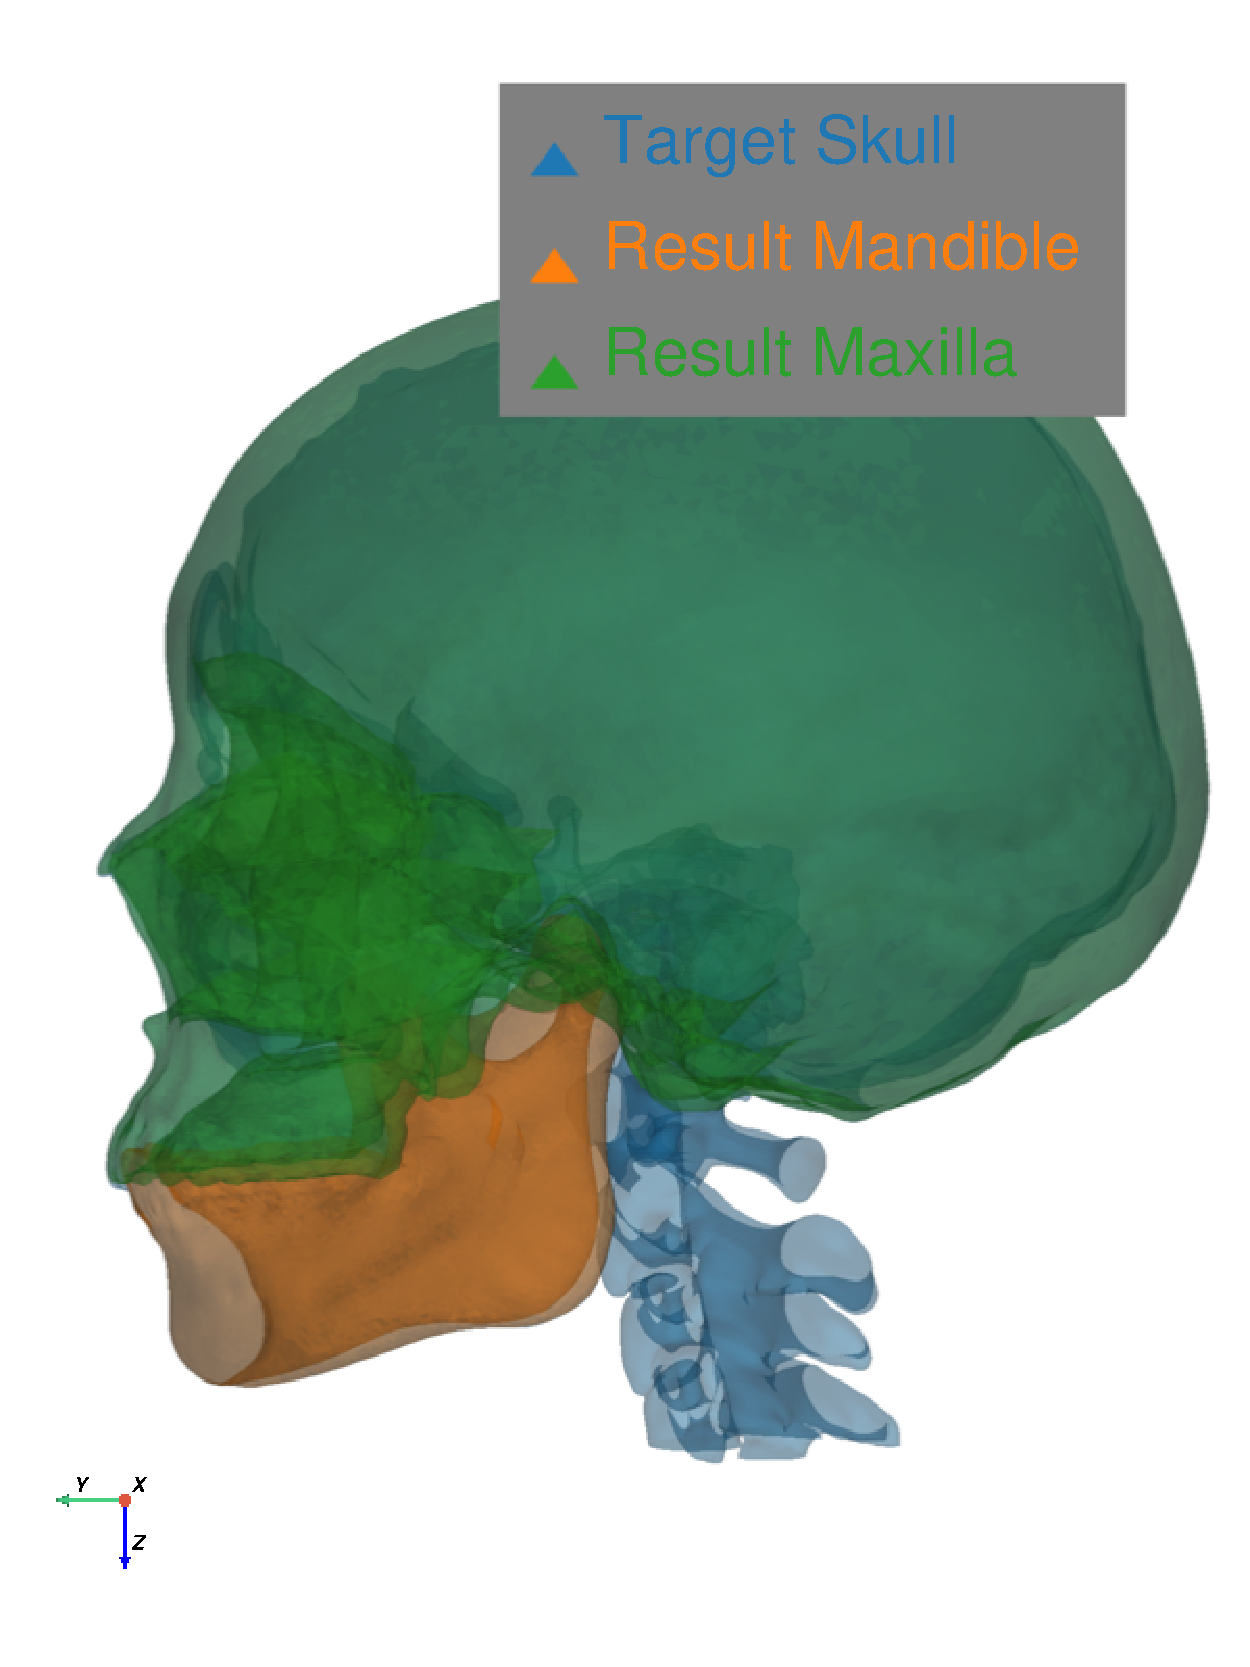
\includegraphics[width = 0.3 \linewidth]{register/register-skull.pdf}}
  \caption{非刚性配准}
  \label{fig:registration}
\end{figure}

\section{四面体网格生成}

在获得模板与患者的三角面网格构型后,我们需将其细分为四面体网格,以适应下一步的仿真分析需求。
在这一过程中,采用了 TetGen 工具 \cite{siTetGenDelaunaybasedQuality2015},其被证实能够生成高品质的四面体网格。
遗憾的是,TetGen 并不能处理含有自相交三角面的输入网格,因此必须对输入模型进行预处理。

我们选用 MeshFix 修复工具 \cite{atteneLightweightApproachRepairing2010},以消除自相交的问题。
修复流程首先独立对面部、上颌骨和下颌骨模型进行处理。
考虑到模板中上下颌骨之间的相交现象,我们将各自修复的结果进行布尔并操作,从而合成一个完整的颅骨模型。
尽管 MeshFix 和布尔操作可能会改变模型的拓扑结构,而不能保证手术前后拓扑结构的一致性,这些变动仅在局部发生。
因此,通过比对手术前和修复后的模型,仍能够识别出拓扑结构保持不变的顶点,利用这些顶点可以追踪手术前后模型之间的对应关系和相应顶点的位移。
至于其余顶点的位移,可通过在 TetGen 所生成四面体网格的骨骼表面插值获得。
鉴于骨骼的刚性特性,我们采用最近邻插值法确保插值结果的准确性。
如图 \ref{fig:tetra} 所示是生成的四面体网格的剖面图。

\begin{figure}
  \centering
  \includegraphics[width = 0.5 \linewidth]{tetra.png}
  \caption{四面体网格剖面}
  \label{fig:tetra}
\end{figure}

% !TeX root = ../thuthesis-example.tex

\chapter{质量-张量模型}

我们使用基于质量-张量模型 (Mass Tensor Model, MTM) \cite{cotinHybridElasticModel2000} 的方法来模拟面部软组织的物理行为.
MTM 可以看作是 MSM 和 FEM 结合的产物.
一方面, MTM 具有与 MSM 相似的简单结构; 另一方面, MTM 具有与 FEM 相仿的生物力学相关性.

MTM 采用 Saint Venant-Kirchhoff 模型, 其应变能密度函数为:
\begin{equation}
  W(E) = \frac{\lambda}{2} (\tr(E))^2 + \mu \tr(E^2)
\end{equation}
其中 $\lambda, \mu$ 为 Lam\`e 参数, $E$ 为 Lagrangian 有限应变张量, 定义为:
\begin{equation}
  E = \frac{1}{2} \pqty{(\grad{u})^T + \grad{u} + (\grad{u})^T \cdot \grad{u}}
\end{equation}
其中 $u$ 表示位移场.
在小位移假设下, Lagrangian 应变张量 $E$ 可线性近似为
\begin{equation}
  E = \frac{1}{2} \pqty{\grad{u} + (\grad{u})^T}
\end{equation}
我们将建模对象离散化为四面体网格.
给定一个四面体 $T_i$ 及其四个顶点在无形变状态下的位置 $\bm{P}_0$, $\bm{P}_1$, $\bm{P}_2$, $\bm{P}_3$.
四面体内部某一点 $\bm{P}$ 的位移场 $\bm{u}$ 可以通过重心坐标线性插值得到:
\begin{equation}
  \bm{u}(\bm{P}) = \sum_{j = 0}^3 \alpha_j \bm{u}(\bm{P}_j)
\end{equation}
其中 $\alpha_j$ 为 $\bm{P}$ 的重心坐标:
\begin{equation}
  \alpha_j(\bm{P}) = - \frac{\bm{M}_j}{6 V_i} \cdot (\bm{P} - \bm{P}_{j + 1})
\end{equation}
其中 $V_i$ 为四面体 $T_i$ 的体积, 向量 $\bm{M}_j$ 由以下等式定义:
\begin{equation}
  \begin{split}
    \bm{M}_j^{T_i} & =
    \begin{bmatrix}
      M_j^x & M_j^y & M_j^z
    \end{bmatrix}
    ^T                                                                                                                                                                     \\
                   & = \bm{P}_{T_i(j + 1)}^0 \cp \bm{P}_{T_i(j + 2)}^0 + \bm{P}_{T_i(j + 2)}^0 \cp \bm{P}_{T_i(j + 3)}^0 + \bm{P}_{T_i(j + 3)}^0 \cp \bm{P}_{T_i(j + 1)}^0
  \end{split}
\end{equation}
$\bm{M}_j^{T_i}$ 具有显然的几何意义, 其方向与 $\bm{P}_{T_i(j)}^{T_i}$ 相对的三角形面片的外法向量相同, 其模长 $\norm{\bm{M}_j^{T_i}}$ 为该三角形面积的两倍.
由此我们可以导出该四面体 $T_i$ 内各顶点受力与位移的关系:
\begin{equation}
  \bm{f}_j^{T_i}
  = - V_i \pdv{W}{\bm{u}_j}
  = \sum_{k = 0}^3 \bm{K}_{jk}^{T_i} \bm{u}_k
\end{equation}
其中 $\bm{K}_{jk}^{T_i}$ 为刚度矩阵, 定义为:
\begin{equation}
  \bm{K}_{jk}^{T_i} = \frac{1}{36 V_i} \pqty{\lambda_i \bm{M}_k^{T_i} (\bm{M}_j^{T_i})^T + \mu_i \bm{M}_j^{T_i} (\bm{M}_k^{T_i})^T + \mu_i (\bm{M}_j^{T_i} \bm{M}_k^{T_i}) \bm{I}_3}
\end{equation}
其中 $V_i$ 为四面体 $T_i$ 的体积, $\lambda_i, \mu_i$ 为四面体 $T_i$ 的 Lam\`e 参数, $\bm{I}_3$ 为 $3 \times 3$ 单位矩阵, $\bm{M}_j^{T_i}$ 的定义如前文所述.
由此可得整个模型的逐顶点受力与位移的关系可表达为:
\begin{equation}
  \bm{f}_j
  = \sum_{T_i} \bm{f}_j^{T_i}
  = \sum_{k \in \Psi_j} \bm{K}_{jk} \bm{u}_k
\end{equation}
其中
\begin{equation}
  \bm{K}_{jk} = \sum_{T_i \in \Lambda_j} \bm{K}_{jk}^{T_i}
\end{equation}
如此, MTM 在质点和四面体网格的简洁表达上, 建立了力与位移之间的线性关系.

回到本文的问题, 我们需要将上述模型应用到正颌手术的模拟中.
为了模拟正颌手术对软组织的影响, 我们需要在力学模型中表达骨骼的变化.
我们假设与骨骼相邻的软组织与骨骼之间的连接是刚性的, 即在软组织与骨骼之间的连接点上, 软组织的位移与骨骼的位移相同.
这部分顶点我们称为固定顶点, 而不与骨骼直接相连的软组织的顶点我们称为自由顶点.
我们已知手术前后的骨骼模型, 因此我们可以通过计算骨骼的位移来计算紧固定顶点的位移.

已知 $\bm{u}_0$ 为固定顶点的位移, 设待求解的自由顶点位移为 $\bm{u}_1$, 则我们可以将整个模型的受力与位移关系表达为:
\begin{equation}
  \begin{bmatrix}
    \bm{K}_{00} & \bm{K}_{01} \\
    \bm{K}_{10} & \bm{K}_{11}
  \end{bmatrix}
  \begin{bmatrix}
    \bm{u}_0 \\
    \bm{u}_1
  \end{bmatrix}
  =
  \begin{bmatrix}
    \bm{f}_0 \\
    \bm{f}_1
  \end{bmatrix}
\end{equation}
在静止状态下, 由于自由顶点不受外力作用, $\bm{f}_1 = \bm{0}$, 可得:
\begin{equation}
  \bm{K}_{10} \bm{u}_0 = - \bm{K}_{11} \bm{u}_1
\end{equation}
由于 $\bm{K}_{10}$ 为稀疏矩阵且并不保证正定, 无法使用直接分解的方法求解, 因此我们使用最小残量迭代法 (MINRES) 来求解上述线性问题.


% 其他部分
\backmatter

% 插图和附表清单
% 本科生的插图索引和表格索引需要移至正文之后、参考文献前
% \listoffiguresandtables  % 插图和附表清单(仅限研究生)
% \listoffigures           % 插图清单
% \listoftables            % 附表清单

% 参考文献
\bibliography{ref/refs.bib}  % 参考文献使用 BibTeX 编译
% \printbibliography       % 参考文献使用 BibLaTeX 编译

% 致谢
% % !TeX root = ../thuthesis-example.tex

\begin{acknowledgements}
  在本次毕业设计论文的撰写过程中,我得到了许多人的关心和帮助。在此,我想借此机会表达我诚挚的感谢。

  首先,我要感谢我的导师徐枫副教授,他在整个研究过程中给予了我无尽的指导和支持。从课题选择、研究思路的确定到论文写作的每一个细节,他都给予了我宝贵的建议和鼓励,使我能够顺利完成这篇论文。

  其次,我要感谢我的同学和朋友们。在我遇到困难和困惑时,是你们的帮助让我保持信心和动力。特别是吕军锋、凌精望、韩宇轩学长,还有邵云哲同学,感谢你们在研究方法和实验过程中提供的帮助和建议。

  此外,我还要感谢我的家人。你们无私的支持和理解让我能够专心投入到学习和研究中。特别是父母,你们的关爱和鼓励是我前进的动力。

  最后,我要感谢清华大学以及软件学院和土木水利学院的各位老师和工作人员,你们提供了良好的学习和研究环境,以及丰富的学术资源,使我能够顺利完成学业。

  衷心感谢所有在这段时间内给予我帮助和支持的人们!
\end{acknowledgements}


% 声明
\statement
% 将签字扫描后的声明文件 scan-statement.pdf 替换原始页面
% \statement[file=scan-statement.pdf]
% 本科生编译生成的声明页默认不加页脚,插入扫描版时再补上;
% 研究生编译生成时有页眉页脚,插入扫描版时不再重复。
% 也可以手动控制是否加页眉页脚
% \statement[page-style=empty]
% \statement[file=scan-statement.pdf, page-style=plain]

% 附录
% 本科生需要将附录放到声明之后,个人简历之前
\appendix
% % !TeX root = ../thuthesis-example.tex

\begin{survey}
\label{cha:survey}

\title{Title of the Survey}
\maketitle


\tableofcontents


本科生的外文资料调研阅读报告。


\section{Figures and Tables}

\subsection{Figures}

An example figure in appendix (Figure~\ref{fig:appendix-survey-figure}).

\begin{figure}
  \centering
  
\includegraphics[width=0.6\linewidth]{example-image-a.pdf}
  \caption{Example figure in appendix}
  \label{fig:appendix-survey-figure}
\end{figure}


\subsection{Tables}

An example table in appendix (Table~\ref{tab:appendix-survey-table}).

\begin{table}
  \centering
  \caption{Example table in appendix}
  \begin{tabular}{ll}
    \toprule
    File name       & Description                                         \\
    \midrule
    thuthesis.dtx   & The source file including documentaion and comments \\
    thuthesis.cls   & The template file                                   \\
    thuthesis-*.bst & BibTeX styles                                       \\
    thuthesis-*.bbx & BibLaTeX styles for bibliographies                  \\
    thuthesis-*.cbx & BibLaTeX styles for citations                       \\
    \bottomrule
  \end{tabular}
  \label{tab:appendix-survey-table}
\end{table}


\section{Equations}

An example equation in appendix (Equation~\eqref{eq:appendix-survey-equation}).
\begin{equation}
  \frac{1}{2 \uppi \symup{i}} \int_\gamma f = \sum_{k=1}^m n(\gamma; a_k) \mathscr{R}(f; a_k)
  \label{eq:appendix-survey-equation}
\end{equation}


\section{Citations}

Example citations in appendix.
\cite{abrahams99tex}
\cite{salomon1995advanced}
\cite{abrahams99tex,salomon1995advanced}


\bibliographystyle{unsrtnat}
\bibliography{ref/appendix}

\end{survey}
       % 本科生:外文资料的调研阅读报告
% % !TeX root = ../thuthesis-example.tex

\begin{translation}
\label{cha:translation}

\title{投影动力学:融合约束投影以实现快速模拟}
\maketitle

\begin{figure}
  \centering
  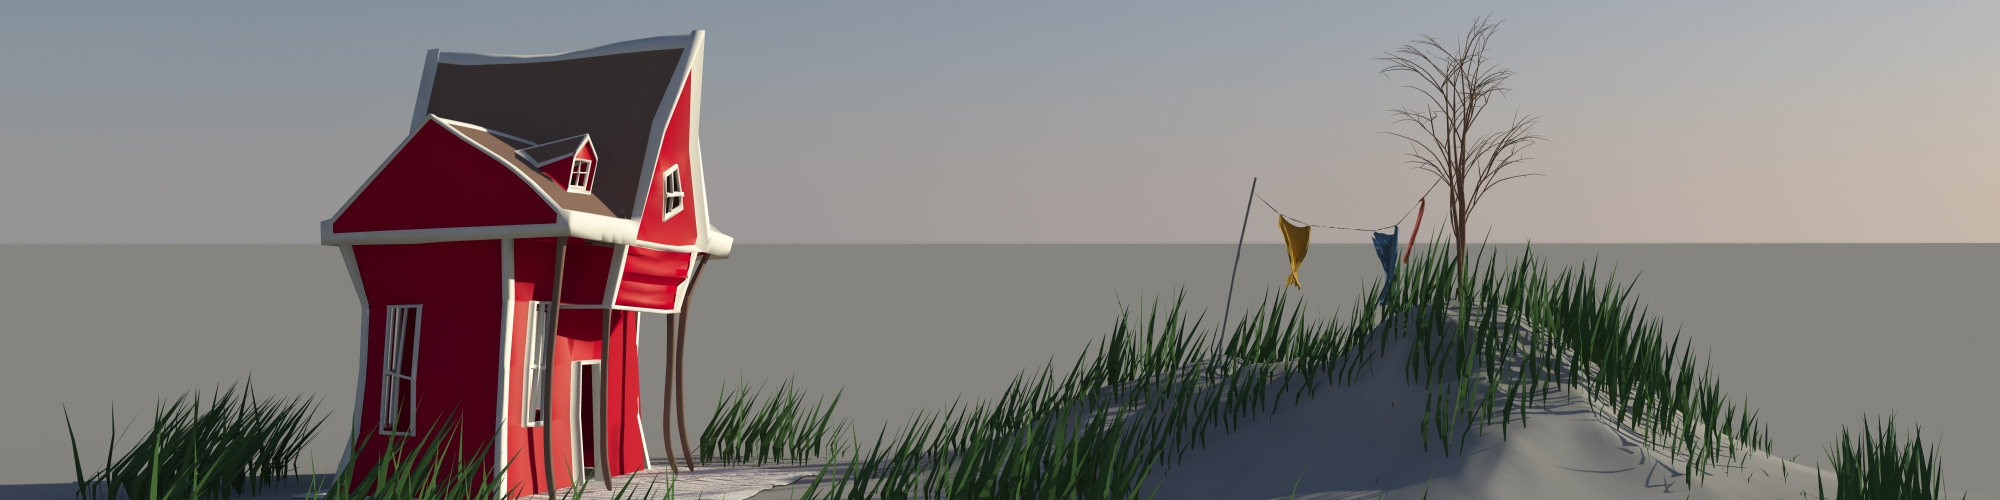
\includegraphics[width = \linewidth]{translation/1.png}
  \caption{
    我们提出了一种新的“基于投影”的隐式Euler积分器,可在单一物理仿真框架中支持多种几何约束。在本示例中,包括建筑物、草地、树木和衣服在内的所有元素(\SI{49}{k}DoFs,\SI{43}{k}约束)都是在\SI{3.1}{\milli\second/iteration}的时间内进行模拟的,每帧迭代10次(另见附带视频)。
  }
  \label{fig:translation-1}
\end{figure}

\begin{abstract}
  我们提出了一种物理系统隐式时间积分的新方法。我们的方法在节点有限元方法和基于位置的动力学之间架起了一座桥梁,从而产生了一种简单、高效、鲁棒而又精确的求解器,支持多种不同类型的约束条件。我们提出了专门设计的势能,可以使用交替优化方法高效求解。受连续介质力学的启发,我们推导出一套基于连续介质的势能,可以有效地集成到我们的求解器中。我们在许多不同的应用中展示了我们方法的通用性和鲁棒性,包括固体、布料和壳体的模拟,以及基于示例的模拟。与牛顿求解器和基于位置的动力学求解器的比较凸显了我们的方法的优势。
\end{abstract}

% \tableofcontents

\section{引言}

基于物理的可变形材料模拟已成为计算机图形学许多领域不可或缺的工具。虚拟世界,以及最近的角色动画,都融入了复杂的模拟以极大地增强视觉体验,例如,通过模拟肌肉、脂肪、头发、衣物或植被。这些模型通常基于连续介质力学公式的有限元离散化,允许高度\emph{精确}地模拟复杂的非线性材料。

除了真实性和准确性,计算机图形学应用中还有许多其他重要的标准。\emph{通用性}是指模拟广泛行为能力的能力,如不同类型的几何体(固体、壳体、杆件)、不同的材料属性,甚至是对经典基于物理的模拟的可控艺术扩展。\emph{鲁棒性}指的是适当处理困难状态的能力,包括大变形、退化几何形状和大时间步长。鲁棒性在实时应用中尤其重要,在这些应用中没有“第二次机会”重新运行模拟,例如在电脑游戏或医学培训模拟器中。求解器的\emph{简单性}对其相关实际应用往往很重要——基于简单、易于理解的概念以及由此产生的轻量级代码库——简化了模拟器的维护,并使其能够适应特定的应用需求。\emph{性能}是实时应用的关键使能标准。然而,在离线模拟中,性能同样重要,应尽量减少测试新场景和模拟参数的周转时间。

当前的连续介质力学方法在计算机图形学应用中的某些方面往往存在不利的权衡,这催生了替代方法的发展,例如基于位置的动力学(PBD)。由于其通用性、简单性、鲁棒性和效率,PBD现在已经在包括PhysX、Havok Cloth、Maya nCloth和Bullet在内的一系列高阶产品中实现。虽然主要用于实时应用,但PBD也经常用于离线模拟。然而,PBD的理想特性是以有限的准确性为代价的,因为PBD并不是从连续体力学原理中严格推导出来的。

我们提出了一种新的隐式积分求解器,它弥合了连续体力学和PBD之间的差距。关键思想是引入具有特定结构的势能。更准确地说,我们的势能由一个凸二次距离度量组成,该度量来自一个\emph{约束}。约束是表达元素期望状态的一般非线性函数,例如,四面体的体积必须保持在给定的范围内。距离度量量化了在给定变形状态中各个约束被违反的程度。虽然我们的求解器可以处理任意的几何约束,但我们提出了一组特定的约束,这些约束源自连续应变能。这些基于连续体的约束非常实用,因为它们大大简化了参数调整,特别是在处理不同分辨率和非均匀细分的网格时。

我们基于约束的势能的主要优势在于,它们的结构使得能够进行高效的局部/全局优化(块坐标下降)。具体来说,局部优化步骤将每个元素投影到约束流形上,即,为每个元素解决一个小的非线性问题。全局优化步骤结合了个体投影的结果,找到所有个体约束之间的折中方案,同时也考虑了全局效应,如惯性和外力。

局部/全局方法使我们能够制定一个隐式积分求解器,它保证在每次迭代中弱减少能量,而不需要任何特定的预防措施。这与经典的牛顿方法相比,后者需要线性搜索策略和防范奇异或不定Hessian矩阵以保证鲁棒性。此外,对于固定的约束集,我们可以预先分解全局步骤的线性系统,这大大减少了计算时间。局部步骤由小的独立优化问题组成,这些问题都可以并行执行。

据我们所知,我们的方法是第一个将局部/全局优化应用于模拟一般动力系统的方法。我们证明了这种解决方案提供了一种鲁棒且高效的隐式积分方法,通常显著优于经典的牛顿方法。PBD与我们的求解器之间的联系揭示了PBD如何与基于有限元方法和牛顿力学的传统方法相关的新见解。

\section{相关工作}

自从Terzopulous及其同事在1987年的开创性工作以来[1987],源自连续介质力学的模型在基于物理的动画中扮演了重要角色。基本原理是,弹性物体对变形的抵抗力是通过弹性势能量化的——一个标量函数,其变分导数导出弹性力[Sifakis and Barbic 2012]。不幸的是,即使是基本的材料模型,弹性力通常也是非线性的,这使得运动方程的时间积分变得复杂。

计算机图形学中使用的最简单的时间积分方案是显式的,对大时间步长非常脆弱[Press et al. 2007]。隐式Euler方法显著提高了鲁棒性[Baraff and Witkin 1998],但代价是在每一步都要解一个非线性方程组。正如[Martin et al. 2011]所示,这可以等效地表述为一个直接作用于弹性势能而非力的非凸优化问题。隐式积分的一个主要缺点是人为的数值阻尼。这启发了辛积分器[Hairer et al. 2002; Kharevych et al. 2006]和混合隐式-显式方法(IMEX)[Bridson et al. 2003; Stern and Grinspun 2009]的发展,它们具有更好的能量守恒特性。另一种方法是\emph{energy budgeting}[Su et al. 2013],它显式地强制能量守恒。然而,隐式Euler积分继续是物理动画应用中的一个受欢迎的选择,其中鲁棒性是一个重要标准,数值阻尼不是主要关注点。我们的求解器是从隐式Euler积分的变分形式[Martin et al. 2011]衍生出来的,因为它为我们的框架中的时间积分提供了一种直观的思考方式——仅仅通过向系统添加另一个约束。这进一步允许我们在PBD和隐式Euler积分方案之间建立联系,并导出一种鲁棒且高效的方法,该方法在大时间步长下稳定。

不管隐式积分的具体形式和表述如何,牛顿法仍然是解决非线性方程组的主要方法。然而,其鲁棒实现需要采取预防措施,如保守的线搜索程序和对不定Hessian的防范[Boyd and Vandenberghe 2004]。从性能的角度来看,牛顿法的一个严重缺点是Hessian矩阵和梯度在每次迭代时都会变化。因此,拟牛顿法采用近似Hessian,用次优的下降方向换来更快的线性系统求解(因此收敛速度更慢),正如[Desbrun et al. 1999; Hahn et al. 2012]所示。在共旋弹性的背景下探索的一种类似策略是使用精心调度的稀疏Cholesky分解更新[Hecht et al. 2012]。最近,Liu及其同事[2013]提出了一种高效隐式时间积分质点-弹簧系统的方法,通过引入辅助变量来实现局部/全局优化的交替。这种方法,也被称为块坐标下降法,之前已在几何处理中取得了巨大成功[Sorkine and Alexa 2007; Bouaziz et al. 2012]。我们的方法也采用了局部/全局交替,但与[Liu et al. 2013]不同的是,后者仅限于质量-弹簧系统,并且\emph{只}假设线性弹簧(胡克定律),我们展示了如何通过将投影概念推广到约束集上来模拟\emph{一般的}节点动力系统。

我们基于约束的公式与基于约束投影的最新非传统方法有些相似。约束投影的概念是Nucleus系统[Stam 2009]和基于位置的动力学[Müller et al. 2007; Bender et al. 2013]的核心。与我们的解决方案不同,这些方法并没有以全局方式处理约束,而是以(非线性的)Gauss-Seidel类似的方式迭代地投影到它们上[Müller et al. 2007]。虽然得到的算法非常容易实现,但这种方法有一些缺点:Gauss-Seidel优化的收敛速度不是很快,材料刚度取决于迭代次数,结果依赖于遍历顺序。相比之下,我们的方法使用约束来制定弹性势能,这些势能与牛顿运动定律所规定的惯性项严格结合。我们的求解器首先分别计算所有约束投影,然后找到它们之间的最佳折衷,这使得解决方案不依赖于约束的顺序。为了获得更快的收敛速度,约束是用微分坐标表示的,这通常在仅几次迭代后就能得到令人满意的结果。此外,与基于位置的动力学不同,我们的求解器收敛到一个真正的隐式Euler解,带有我们的弹性能量,而基于位置的动力学收敛到完全无弹性的行为。

另一个与我们的方法密切相关的概念是形状匹配[Müller et al. 2005; Rivers and James 2007],与我们的方法不同的是,约束投影被用来直接构建弹性力而不是势能来模拟可变形物体。约束投影也被用于\emph{应变限制}[Provot 1995; Goldenthal et al. 2007; Thomaszewski et al. 2009; Wang et al. 2010; Narain et al. 2012],不是作为一种独立的模拟技术,而是作为一种改善标准时间积分方法处理刚性系统的方式。在我们的方法中,我们也可以进行应变限制,但它直接包含在隐式求解器中。

\section{连续介质力学视角}

在本节中,我们将介绍我们方法的基础——我们势能的特殊结构。我们从有限元素法离散的弹性模型的隐式时间积分开始。

\subsection{隐式Euler求解器}

让我们简要回顾一下隐式Euler积分的变分形式[Martin et al. 2011]。我们假设一个由$m$个顶点组成的网格,顶点位置为$\vb{q} \in \mathbb{R}^{m \times 3}$,速度为$\vb{v} \in \mathbb{R}^{m \times 3}$。系统根据牛顿运动定律在一系列离散的时间点$t_1, t_2, \dots$中随时间演化。在时间$t_n$,系统可由$\{\vb{q}_n, \vb{v}_n\}$确定。外力之和为$\vb{f}_{\text{ext}}$,内力之和为$\vb{f}_{\text{int}}$。我们考虑位置依赖的内力,即$\vb{f}_{\text{int}}(\vb{q}) = - \sum_i \grad{W_i(\vb{q})}$,其中$W_i(\vb{q})$是一个标量势能函数。隐式Euler时间积分导出以下更新规则:
\begin{gather}
  \vb{q}_{n + 1} = \vb{q}_n + h \vb{v}_{n + 1} \label{eq:translation-1} \\
  \vb{v}_{n + 1} = \vb{v}_n + h \vb{M}^{-1} (\vb{f}_{\text{int}}(\vb{q}_{n + 1}) + \vb{f}_{\text{ext}}) \label{eq:translation-2}
\end{gather}
其中$\vb{M}$是质量矩阵,$h$代表时间步长。注意,$\vb{f}_{\text{ext}}$和$\vb{M}$在任何给定的时间步长中都是保持不变的。使用这些公式,我们可以推导出
\begin{equation}
  \vb{M} (\vb{q}_{n + 1} - \vb{q}_n - h \vb{v}_n) = h^2 (\vb{f}_{\text{int}}(\vb{q}_{n + 1}) + \vb{f}_{\text{ext}})
  \label{eq:translation-3}
\end{equation}
这个系统可以转换为一个优化问题
\begin{equation}
  \min_{\vb{q}_{n + 1}} \frac{1}{2 h^2} \norm{\vb{M}^{\frac{1}{2}} (\vb{q}_{n + 1} - \vb{s}_n)}_F^2 + \sum_i W_i(\vb{q}_{n + 1})
  \label{eq:translation-4}
\end{equation}
其中$\vb{s}_n = \vb{q}_n + h \vb{v}_n + h^2 \vb{M}^{-1} \vb{f}_{\text{ext}}$,$\norm{\cdot}_F$表示Frobenius范数。直观上,这个最小化问题也即\emph{动量势能}
\begin{equation}
  \frac{1}{2 h^2} \norm{\vb{M}^{\frac{1}{2}} (\vb{q}_{n + 1} - \vb{s}_n)}_F^2
  \label{eq:translation-5}
\end{equation}
这表明解应该遵循其动量(加上外力),以及要求解最小化弹性形变的弹性势能之间的折中。相应的权重项,即$\vb{M}$中的质量分布、时间步长$h$和材料刚度$W$,决定了这种平衡中哪个势能更重要。此外,根据Noether定理,当弹性势能对刚体运动是不变的时,线性和角动量总是守恒的。

公式\eqref{eq:translation-4}的最小化通常使用精心实现的牛顿法来执行[Martin et al. 2011]。然而,这是相当昂贵的,因为在每次迭代中都需要解一个不同的线性系统,因为Hessian从一次迭代到下一次迭代是变化的。为了简化表示,我们将在下文中省略$\vb{q}_{n + 1}$的下标,只使用 $\vb{q}$。

\subsection{非线性弹性力学}

我们分析了基于有限元方法(FEM)的非线性弹性能量的经典形式,以揭示我们如何限制公式\eqref{eq:translation-4}中的弹性势能,以便推导出我们的新型求解器。

\paragraph{非线性弹性势能。}

在非线性连续介质力学中,从静止状态开始的变形是使用离散的元素应变$\vb{E}(\vb{q})$来衡量的,例如,二次Green应变[Irving et al. 2004]。实践中使用的许多弹性势均使用(通常是非线性的)材料模型$\Psi(\cdot)$将其公式化为应变的函数,从而得到弹性势$W(\vb{q}) = \Psi(\vb{E}(\vb{q}))$。从几何角度来看,我们可以观察到$\vb{E}(\vb{q}) = \vb{0}$定义了所有可能未变形状态的约束流形,而$\Psi(\vb{E}(\vb{q}))$度量变形状态与该流形的距离(图~\ref{fig:translation-2}中的等值线)。我们的关键观察是这两个概念可以解耦;距离度量不必是一个复杂的非线性函数,因为非线性已经包含于约束流形。

\begin{figure}
  \centering
  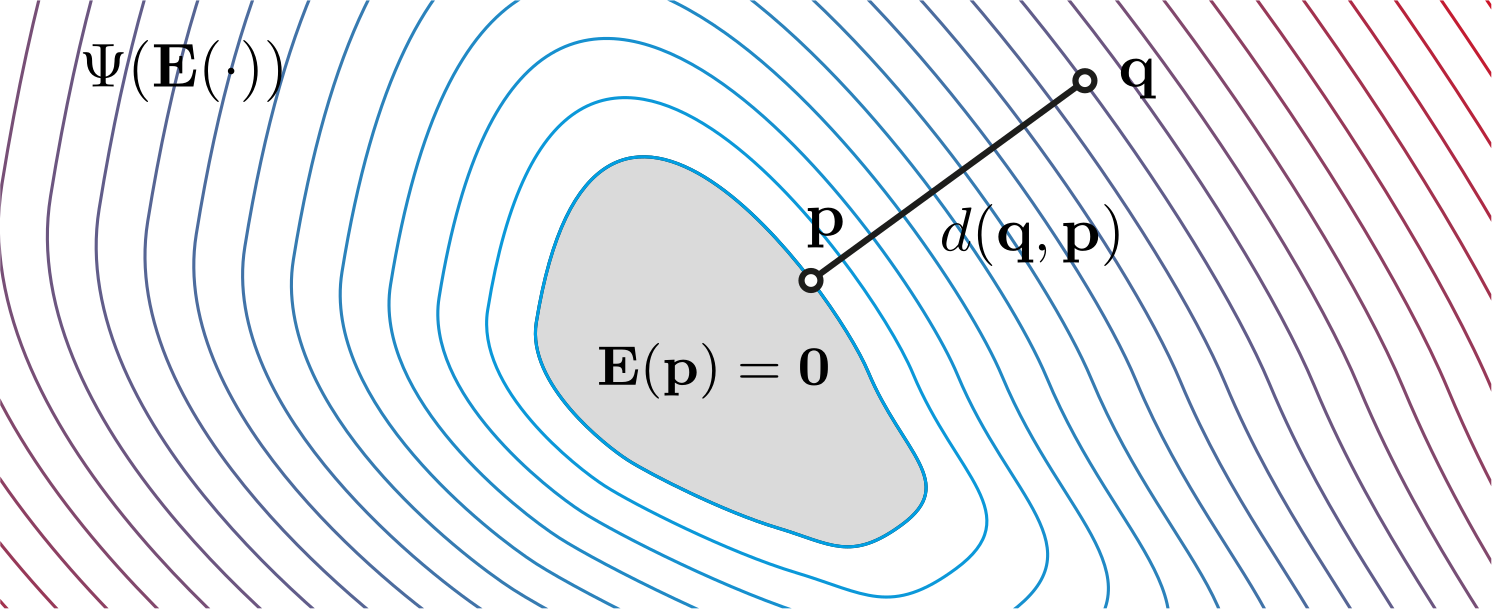
\includegraphics[width = 0.5 \linewidth]{translation/2.png}
  \caption{
    函数$\Psi(\vb{E}(\cdot))$既定义了约束流形$\vb{E}(\cdot) = \vb{0}$作为其零水平集,也定义了由其等值线给出的弹性势能。通过在流形中引入一个投影变量$\vb{p}$,我们可以将流形定义与弹性势能解耦,后者被建模为距离函数$d(\vb{q}, \vb{p}$)。
  }
  \label{fig:translation-2}
\end{figure}

\paragraph{解耦距离度量和约束流形。}

我们引入了使用辅助变量$\vb{p}$的势能函数$W$,定义为
\begin{equation}
  W(\vb{q}, \vb{p}) = d(\vb{q}, \vb{p}) + \delta_{\vb{E}}(\vb{p})
  \label{eq:translation-6}
\end{equation}
这里,$\delta_{\vb{E}}(p)$是一个指示函数,如果$\vb{E}(\vb{p}) = 0$则为零,否则为$+\infty$,并且规定了$\vb{p}$应该位于约束流形上。然后函数$d(\vb{q}, \vb{p})$度量$\vb{q}$和$\vb{p}$之间的距离。关于$\vb{p}$最小化公式\eqref{eq:translation-6}相当于将$\vb{q}$投影到约束流形上,如图~\ref{fig:translation-2}所示。因此,可以定义一个类似于$\Psi(\vb{E}(\vb{q}))$的弹性势能为$W(\vb{q}) = \min_{\vb{p}} W(\vb{q}, \vb{p})$。

\paragraph{二次距离度量。}

考虑到这种解耦,我们可以构建一个求解器,它交替进行距离最小化和投影。这种方法的一个重要优势是距离度量可以自由选择。\emph{约束的非线性}(也称为几何非线性)已经通过对约束集的投影得到处理,因此距离度量可以保持简单,以效率和鲁棒性为代价,而不考虑一般\emph{材料的非线性}。具体来说,我们基于距离矩阵导出以下势能:
\begin{equation}
  W(\vb{q}, \vb{p} = \frac{w}{2} \norm{\vb{A} \vb{q} - \vb{B} \vb{p}}_F^2 + \delta_{\vb{C}(\vb{p})})
  \label{eq:translation-7}
\end{equation}
其中$\vb{A}$和$\vb{B}$是常数矩阵,$w$是非负权重。因此,到约束集的距离通过$\vb{q}$和$\vb{p}$的\emph{二次}函数来建模,这使我们能够使用一个高效的求解器。此外,我们不限于使用Green应变,而可以使用任何约束定义$\vb{C}(\vb{q}) = \vb{0}$来表示所需的状态[Baraff and Witkin 1998],例如,描述三角形之间期望的弯曲角度,四面体的目标体积,或后文所讨论的边界条件。

\subsection{投影隐式Euler求解器}

使用简化的势能,如公式\eqref{eq:translation-7}所示,我们可以将公式\eqref{eq:translation-4}中定义的隐式积分重构为关于$\vb{q}$和辅助变量$\vb{p}_i$最小化
\begin{equation}
  \frac{1}{2 h^2} \norm{\vb{M}^{\frac{1}{2}} (\vb{q} - \vb{s}_n)}_F^2 + \sum_i \frac{w_i}{2} \norm{\vb{A}_i \vb{S}_i \vb{q} - \vb{B}_i \vb{p}_i}_F^2 + \delta_{\vb{C}_i}(\vb{p}_i)
  \label{eq:translation-8}
\end{equation}
其中$\vb{S}_i$是一个恒定的选择矩阵,用于选择参与第$i$个约束的顶点。我们使用局部/全局交替最小化技术来最小化公式\eqref{eq:translation-8}。

\paragraph{局部求解。}

首先,我们在保持位置固定的情况下,对辅助变量进行公式\eqref{eq:translation-8}的最小化。由于每个约束都有自己的一组辅助变量$\vb{p}_i$,所以可以独立地对每个约束进行最小化,即
\begin{equation}
  \min_{\vb{p}_i} \frac{w_i}{2} \norm{\vb{A}_i \vb{S}_i \vb{q} - \vb{B}_i \vb{p}_i}_F^2 + \delta_{\vb{C}_i}(\vb{p}_i)
  \label{eq:translation-9}
\end{equation}
这允许局部步骤的大规模并行化。我们将在第~\ref{sec:translation-continuum-based-constraints}节讨论具体的约束类型。

\paragraph{全局求解。}

其次,我们在保持辅助变量固定的情况下,对位置进行公式\eqref{eq:translation-8}的最小化。由于未知数$\vb{q}$在公式\eqref{eq:translation-8}中是二次的,我们可以通过单次线性求解来最小化它。令临界点处梯度消失,导出线性系统
\begin{equation}
  \pqty{\frac{\vb{M}}{h^2} + \sum_i w_i \vb{S}_i^T \vb{A}_i^T \vb{A}_i \vb{S}_i} \vb{q} = \frac{\vb{M}}{h^2} \vb{s}_n + \sum_i w_i \vb{S}_i^T \vb{A}_i^T \vb{B}_i \vb{p}_i
  \label{eq:translation-10}
\end{equation}
只要约束不变,系统矩阵就是常数,因此可以在初始化时预分解,从而实现非常高效的全局求解。右侧需要在每次迭代后更新投影变量后重新计算。请注意,目标函数是有下界的,而且局部和全局步骤都保证减小它,即使对于非凸集也是如此。因此,优化会收敛,使得不需要额外的安全措施。

\paragraph{算法。}

我们在算法~\ref{alg:translation-1}中总结了我们的优化程序。在第~\ref{alg:translation-1L2}行,我们使用估计动量$\vb{s}_n$来初始化。我们观察到,当只使用少量求解器迭代时,这是有利的,因为它导致的系统阻尼比使用上一个时间步的解作为起点时要小。在求解了多次局部/全局迭代后,速度在第~\ref{alg:translation-1L9}行更新。

\begin{algorithm}
  \caption{投影隐式Euler求解器}
  \label{alg:translation-1}
  \small
  \begin{algorithmic}[1]
    \STATE $\vb{s}_n = \vb{q}_n + h \vb{v}_n + h^2 \vb{M}^{-1} \vb{f}_{\text{ext}}$
    \STATE $\vb{q}_{n + 1} = \vb{s}_n$ \label{alg:translation-1L2}
    \FOR{$iter = 0$ \TO solverIteration}
    \FORALL{constraints $i$}
    \STATE $\vb{p}_i = ProjectOnConstraintSet(\vb{C}_i, \vb{q}_{n + 1})$ \label{alg:translation-1L5}
    \ENDFOR
    \STATE $\vb{q}_{n + 1} = SolveLinearSystem(\vb{s}_n, \vb{p}_1, \vb{p}_2, \vb{p}_3, \dots)$ \label{alg:translation-1L7}
    \ENDFOR
    \STATE $\vb{v}_{n + 1} = (\vb{q_{n + 1} - \vb{q}_n}) / h$ \label{alg:translation-1L9}
  \end{algorithmic}
\end{algorithm}

\paragraph{$\vb{A}$和$\vb{B}$的选取。}

如果我们选取$\vb{A}_i = \vb{B}_i = \vb{I}$,公式\eqref{eq:translation-7}度量的是从$\vb{S}_i \vb{q}$到约束集上最近点的欧式平方距离。由于矩阵是对角的,全局求解的Hessian最终也是对角的,因此可以求解一个简单的线性系统。

如果我们利用内部物理约束是平移不变的事实(即,对约束中涉及的所有点应用共同的平移不会改变约束的值),那么收敛速度可以大大提高。在这种情况下,我们可以选择$\vb{A}_i = \vb{B}_i$作为微分坐标矩阵(它们的零空间中有全局平移)。可以使用各种这样的矩阵,例如可以减去平均值[Bouaziz et al. 2012],或者简单地减去约束中涉及的一个顶点[Liu et al. 2013]。请注意,$\vb{A}_i$ 和 $\vb{B}_i$的选择只影响数值求解过程,并不影响动量守恒。

使用这样的微分坐标大大提高了结果局部/全局求解器的收敛速度[Bouaziz et al. 2012]。然而,如果不采取进一步的预防措施,所得到的行为将依赖于分割和分辨率。我们在第~\ref{sec:translation-continuum-based-constraints}节展示,在某些情况下,$\vb{A}_i$和$\vb{B}_i$矩阵可以从连续体公式中导出,以避免这些缺点。

\section{基于位置的动力学视角}
\label{sec:translation-position-based-dynamics-view}[Liu et al. 2013]揭示了一般变分隐式Euler方法与基于位置的动力学(PBD)之间的相似性,在本节中,我们不仅推导出隐式Euler方法与PBD之间的确切关系,而且还推导出局部/全局公式与PBD之间的关系,适用于一般约束。这一分析突出了PBD与我们的求解器之间的紧密联系,但也指出了根本的差异,这些差异解释了我们的方法获得更高精度结果的原因。

\subsection{Gauss-Seidel求解器}
\label{sec:translation-gauss-seidel-solver}

经典的PBD求解器[Müller et al. 2007]执行三个步骤。在第一步中,通过显式Euler步骤初始化位置,忽略内部力。在第二步中,通过连续对每个约束集进行投影来更新位置,同时考虑质量加权。在最后一步中,速度被更新为$\vb{v}_{n + 1} = (\vb{q}_{n + 1} - \vb{q}_n) / h$。

我们可以证明,PBD的约束求解策略实际上实现了对能量的Gauss-Seidel类型最小化
\begin{equation}
  \frac{1}{2} \sum_i \norm{\vb{M}_i^{\frac{1}{2}} (\vb{S}_i \vb{q} - \vb{p}_i)}_F^2 + \delta_{C_i}(\vb{p}_i)
  \label{eq:translation-11}
\end{equation}
这里使用了一个仅涉及约束点的集中质量矩阵$\vb{M}_i$。Gauss-Seidel方法通过顺序优化每个求和项来最小化这个能量,即,最小化形如$\frac{1}{2} \norm{\vb{M}^{\frac{1}{2}} \Delta\vb{q}}_F^2 + \delta_C(\vb{q} + \Delta\vb{q})$的势能,我们引入修正$\Delta\vb{q} = \vb{p} - \vb{q}$来简化推导。使用拉格朗日乘数对线性化约束$C(\vb{q}) + \tr(\grad{C(\vb{q})}^T \Delta\vb{q}) = 0$,我们可以定义拉格朗日量
\begin{equation}
  \frac{1}{2} \norm{\vb{M}^{\frac{1}{2}} \Delta\vb{q}}_F^2 + \lambda \pqty{C(\vb{q}) + \tr(\grad{C(\vb{q})}^T \Delta\vb{q})}
\end{equation}
使用关于$\Delta\vb{q}$的临界点条件,我们找到最优方向$\Delta\vb{q} = - \lambda \vb{M}^{-1} \grad{C(\vb{q})}$。然后可以通过要求线性化约束在这个方向上消失来找到拉格朗日乘数$\lambda$,即,$C(\vb{q}) - \lambda \norm{\vb{M}^{-\frac{1}{2}} \grad{C(\vb{q})}}_F^2 = 0$,最终导出增量
\begin{equation}
  \Delta\vb{q} = - \vb{M}^{-1} \grad{C(\vb{q})} \frac{C(\vb{q})}{\norm{\vb{M}^{-\frac{1}{2}} \grad{C(\vb{q})}}_F^2}
\end{equation}
这与PBD的质量加权更新规则完全相同[Bender et al. 2013]。

\paragraph{讨论。}

理论上,Gauss-Seidel具有良好的收敛性,但这仅适用于可行的约束集。对于不可行的集合,由于缺乏对优化问题的全局视角,Gauss-Seidel会在不兼容的集合之间振荡(见图~\ref{fig:translation-3})。例如,在模拟具有拉伸约束和边界条件或碰撞的弹性材料的压缩时,约束可能变得不可行,因此解将振荡且不会收敛。

\begin{figure}
  \centering
  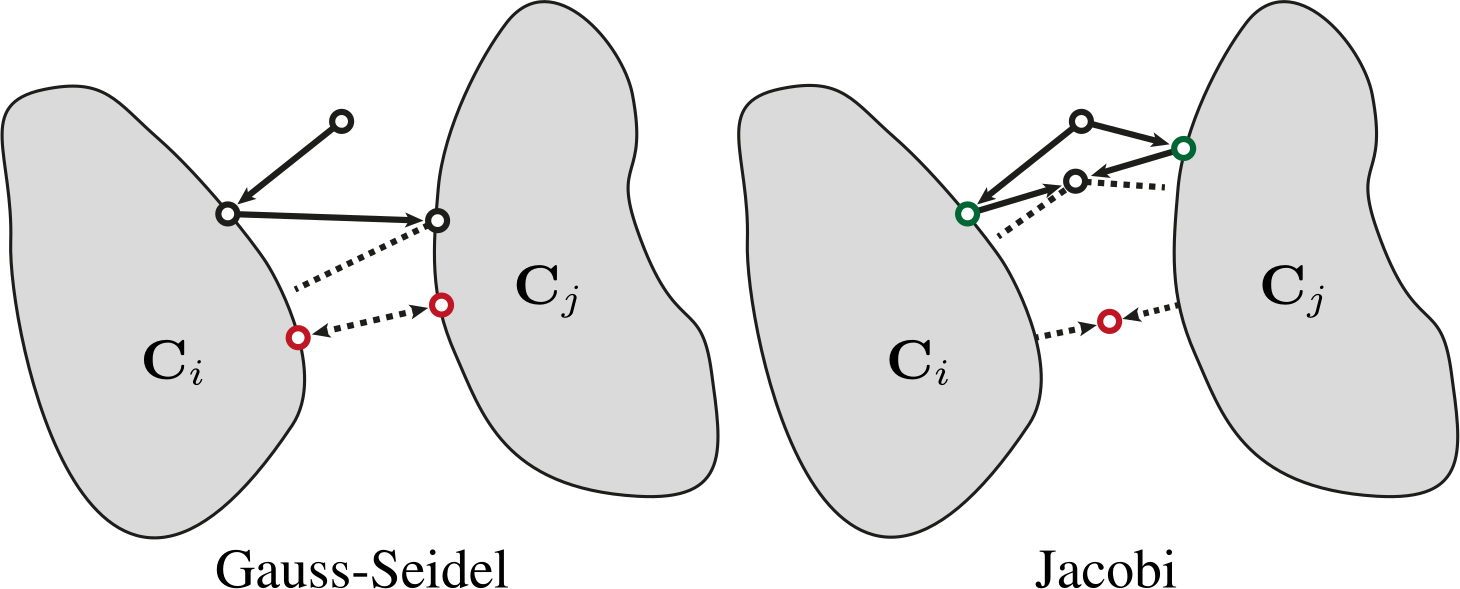
\includegraphics[width = 0.5 \linewidth]{translation/3.png}
  \caption{
    Gauss-Seidel算法与Jacobi算法。PBD中使用的Gauss-Seidel算法会将当前估计值连续投影到每个约束集(本例中为$\vb{C}_i$和$\vb{C}_j$)上。如果没有可行解,即约束集没有重叠,Gauss-Seidel算法就会在不同的约束之间(两个红点之间)摆动。相反,Jacobi算法会将当前估计值并行投影到每个约束集上(绿点),并在第二步折中。这样Jacobi算法就会收敛(红点)。
  }
  \label{fig:translation-3}
\end{figure}

更严重的是,第一步中执行的动量估计也是如此,它包括首先求解方程\eqref{eq:translation-5}中给出的约束。如果将其作为真正的约束添加到优化中,可能会导致完全不兼容的约束集,使收敛性变得更糟。通过首先用初始显式Euler步骤求解动量约束,可以保持整个物体的线性动量,然而,随着优化迭代的时间越长,点的个别动量就会被消除——这与我们提出的隐式Euler求解器建议的在动量和内部弹性之间寻找折中相反(见图~\ref{fig:translation-4})。

\begin{figure}
  \centering
  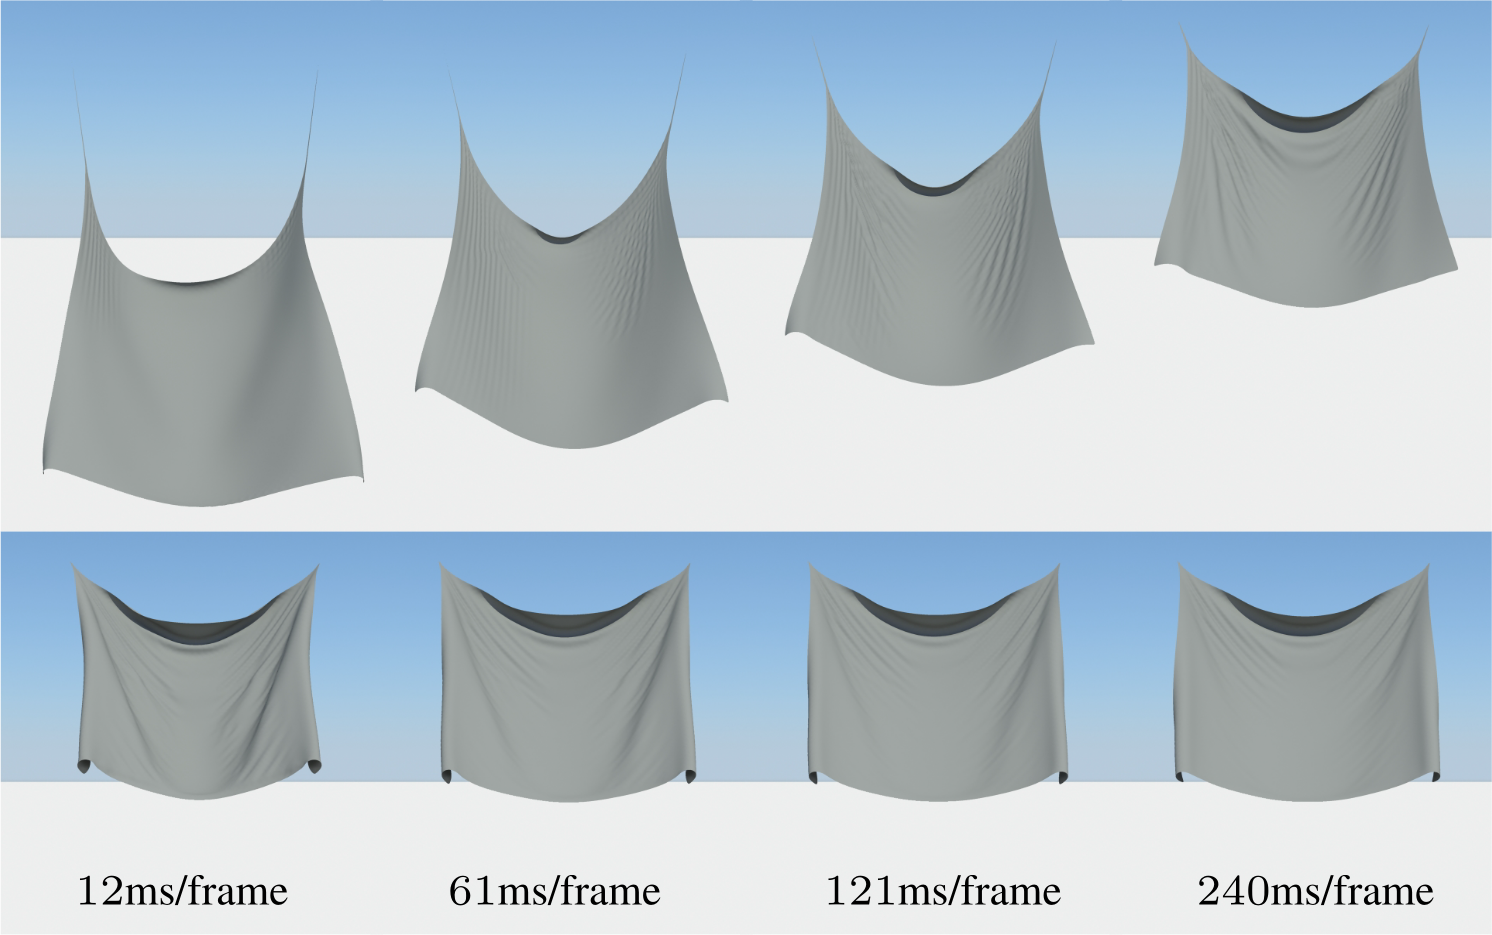
\includegraphics[width = 0.5 \linewidth]{translation/4.png}
  \caption{
    对于一块具有\num{19683}个自由度和\num{19360}个边约束的布料,PBD会根据时间步的允许时间预算显示出不同的材料刚度(上图)。由于额外的动量项和微分坐标表述,即使迭代次数不同,我们的模拟结果也是一致的(下图)。
  }
  \label{fig:translation-4}
\end{figure}

\subsection{Jacobi求解器}

从公式\eqref{eq:translation-11}来看,我们可以通过执行两个步骤以直接的方式求解这些问题。首先,我们用能够处理不兼容约束的Jacobi求解器(见图~\ref{fig:translation-3})替换Gauss-Seidel求解器。一般而言,Jacobi求解器的收敛速度比Gauss-Seidel求解器慢[Thomaszewski et al. 2009]。然而,它们允许使用差分坐标表示法来加快收敛速度,并且能够高效地并行化求解约束投影,从而克服了这一缺点。其次,我们将动量约束引入优化中,以考虑每个点的惯性。正如在连续介质力学视角中看到的,为了实现正确的过程,我们需要通过整合公式\eqref{eq:translation-5}中定义的动量约束项来加回每个点的惯性
\begin{equation}
  \frac{1}{2 h^2} \norm{\vb{M}^{\frac{1}{2}} (\vb{q} - \vb{s}_n)}_F^2 + \sum_i \frac{w_i}{2} \norm{\vb{M}_i^{\frac{1}{2}} (\vb{S}_i \vb{q} - \vb{p}_i)}_F^2 + \delta_{\vb{C}_i}(\vb{p}_i)
  \label{eq:translation-14}
\end{equation}
这样,Jacobi求解器变成了一个两步优化过程:在局部步骤中,首先将当前解$\vb{q}$独立地投影到约束上,通过最小化公式\eqref{eq:translation-11}对所有$\vb{p}_i$进行求解。然后,通过求解关于$\vb{q}$的全局优化,可以在不同解之间达成折中。

\paragraph{与投影隐式Euler法的联系。}

在这一节,我们可以看到这个Jacobi求解器与我们在上一节中介绍的投影隐式求解器程序有多么接近——我们通过选择$\vb{A}_i = \vb{B}_i = \vb{M}_i^{\frac{1}{2}}$来导出这个求解器。通过在下一节中从连续体力学原理导出约束,我们进一步实现了比在PBD中使用的简单基于质量的加权更好的网格剖分独立性和收敛性(见图~\ref{fig:translation-5})。

\begin{figure}
  \centering
  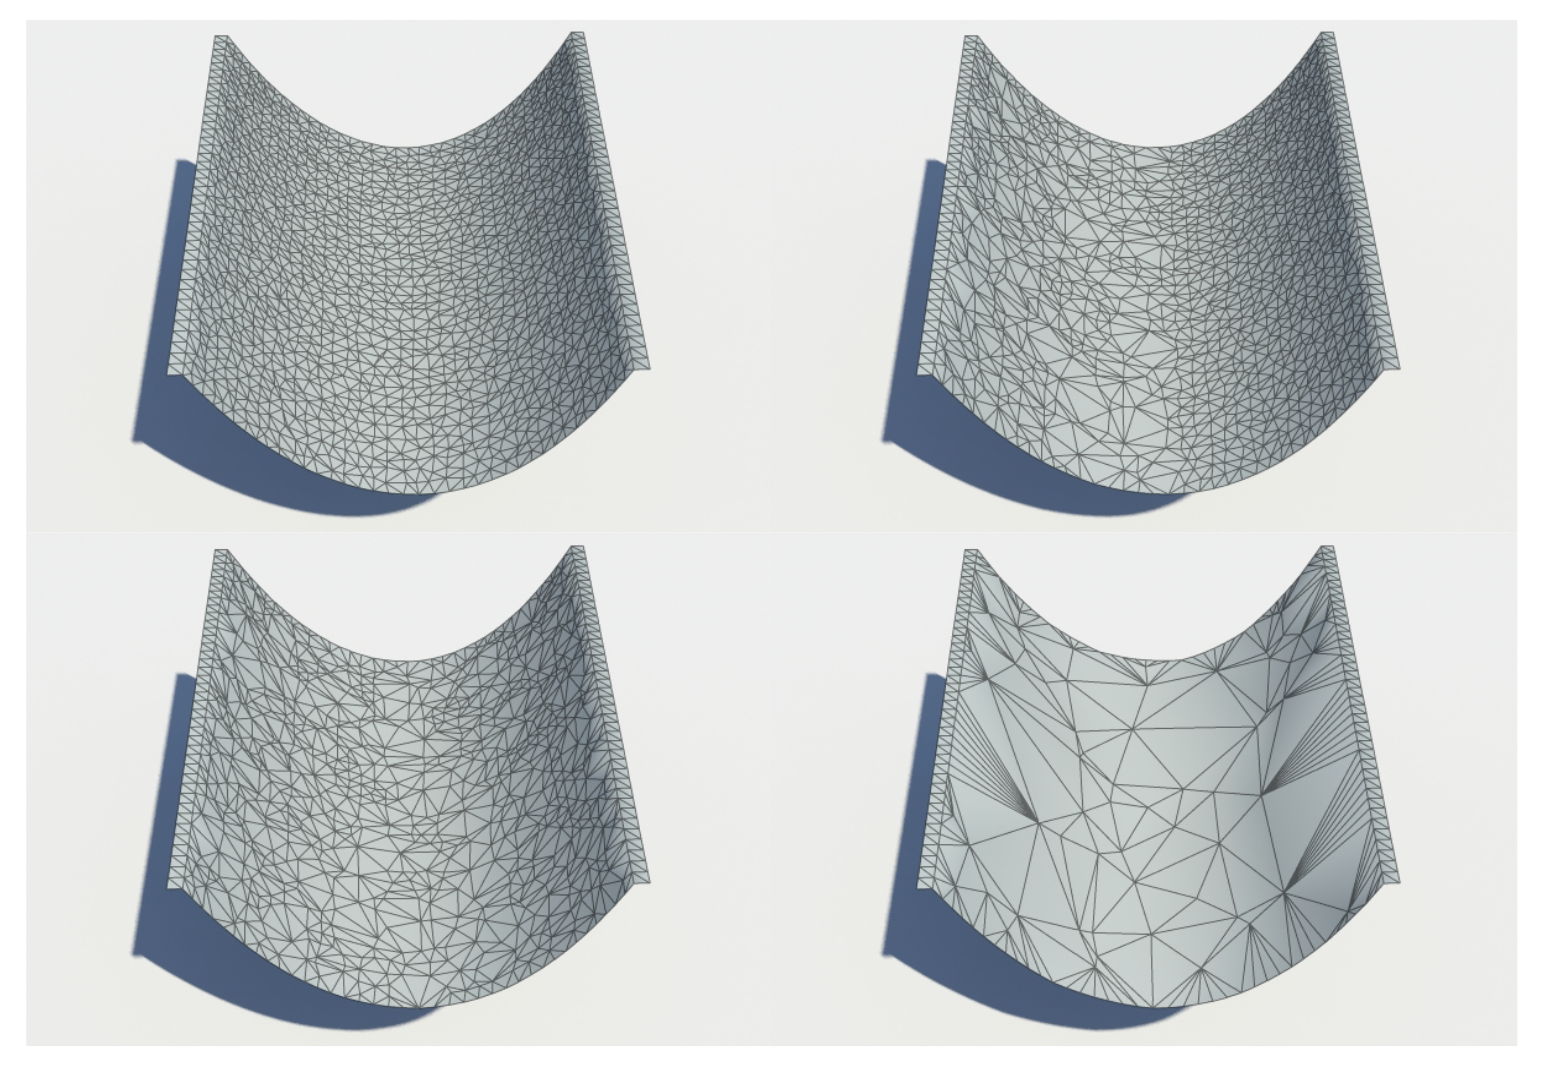
\includegraphics[width = 0.5 \linewidth]{translation/5.png}
  \caption{
    对于给定的连续表面,将我们基于连续性的约束条件离散到不同分辨率的片状简约近似值上,会产生非常相似的定性行为。
  }
  \label{fig:translation-5}
\end{figure}

\section{基于连续介质的约束}
\label{sec:translation-continuum-based-constraints}

微分表示对于我们的局部/全局求解器来提高收敛性是非常重要的。在几何处理中,梯度和Laplace-Beltrami算子在设计高效且鲁棒的模型中扮演着至关重要的角色。在本节中,我们将介绍一组基于这些算子的连续体能量,这些能量允许控制材料在变形过程中的微分属性。我们将展示它们的离散化将具有类似于公式\eqref{eq:translation-7}的形式,这允许在网格细化和非均匀离散化下保持正确的行为。离散势能的局部优化将在附录~\ref{sec:translation-local-solves}中讨论。

\subsection{应力}

\paragraph{连续体能量}

应变能对于模拟可伸展材料至关重要。我们首先讨论2-流形表面,然后将结果扩展到体和曲线。设未变形表面为嵌入$\mathbb{R}^3$中的可微2-流形表面$S$。我们定义未变形表面的分段线性坐标函数为$\vb{g} : S \to \mathbb{R}^3$,及其变形后的对应函数为$\vb{f} : S \to \mathbb{R}^3$。引入一组期望的逐点变换$\vb{T}$ 的集合 $M$,我们构建了一个能量,用以衡量变形和未变形表面之间局部变化的差异,即
\begin{equation}
  E(\vb{f}, \vb{T}) = \frac{w}{2} \int_S \norm{\grad_S{\vb{f}} - \vb{T} \grad_S{\vb{g}}}_F^2 + \delta_M(\vb{T}) \dd{A}
  \label{eq:translation-15}
\end{equation}
其中$\grad_S$是定义在流形表面$S$上的梯度算子。$M$的选择决定了所有允许的静止状态$\vb{T} \grad_S{\vb{g}}$。如果$M$是旋转矩阵集$SO(3)$,我们只是在测量局部偏离刚体运动的程度。在这种情况下,这个能量与Chao等人[2010]提出的变形模型是相同的。如果$M$是具有有界奇异值$\sigma_{\min} < \sigma < \sigma_{\max}$的矩阵集,我们也可以实现类似于Wang等人[2010]的\emph{各向同性应变限制}。这可以进一步扩展到各向异性材料,使用Hernandez等人[2013]提出的参考框架。

\paragraph{离散势能}

如果$S$是一个2-流形单纯复形,这种能量可以通过使用分段线性帽基函数[Botsch et al. 2010]在三角形上离散化。然后,积分被转换为每个三角形势能的求和形式
\begin{equation}
  W(\vb{q}, \vb{T}) = \frac{w}{2} A \norm{\vb{X}_{\vb{f}} \vb{X}_{\vb{g}}^{-1} - \vb{T}}_F^2 + \delta_M(\vb{T})
  \label{eq:translation-16}
\end{equation}
其中$A$是三角形面积,$\vb{X}_{\vb{f}} = [\vb{q}_j - \vb{q}_i, \vb{q}_k - \vb{q}_i] \in \mathbb{R}^{2 \times 2}$包含当前状态中保距嵌入2D的三角形边,类似地$\vb{X}_{\vb{g}}$包含静止状态的三角形边。注意,这个离散势能的形式与公式\eqref{eq:translation-7}中的形式相同,其中$\vb{A}$是静止状态边和面积的函数,而$\vb{B}$仅依赖于静止状态的面积。图~\ref{fig:translation-6}展示了应用于窗帘示例的应变限制约束。

\begin{figure}
  \centering
  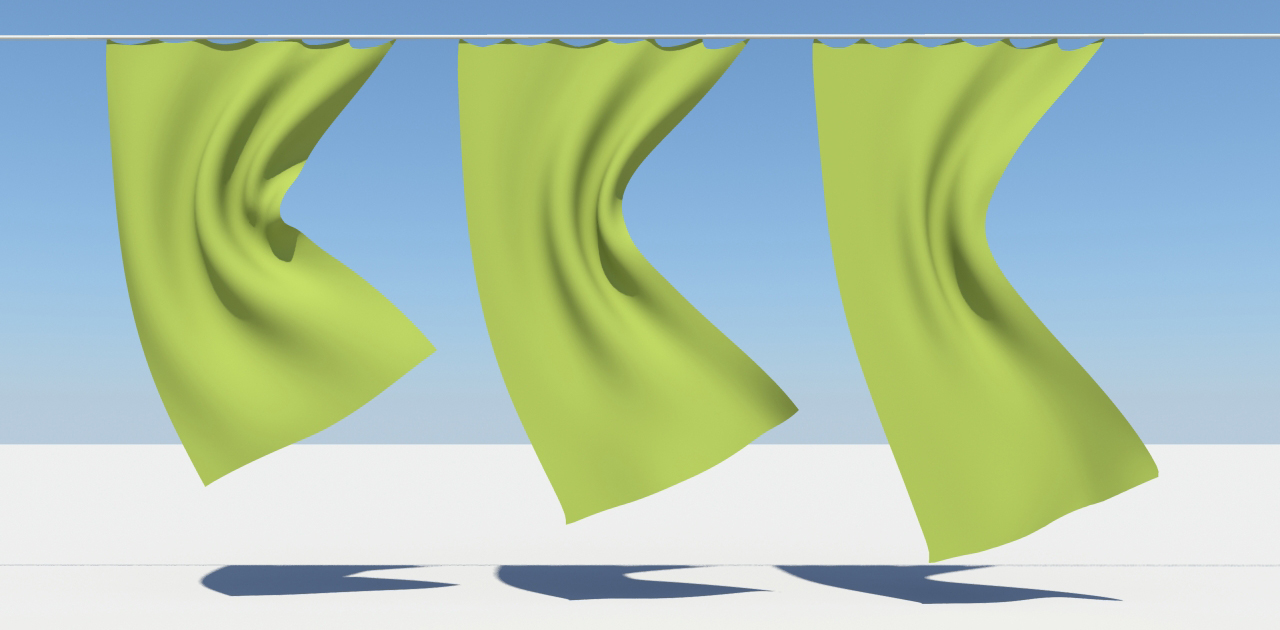
\includegraphics[width = 0.5 \linewidth]{translation/6.png}
  \caption{
    从相同的网格开始,应变限制可以模拟可以承受小到中等程度拉伸的材料。从左到右,我们使用的应变限制分别为$[\SI{-10}{\percent}, \SI{+10}{\percent}]$、$[\SI{-20}{\percent}, \SI{+20}{\percent}]$和$[\SI{-30}{\percent}, \SI{+30}{\percent}]$。请注意,当极限值增加时,布会如何拉伸以及褶皱如何被吸收。
  }
  \label{fig:translation-6}
\end{figure}

\paragraph{体和曲线。}

体的势能可以以类似的方式定义:如果$S$是一个3-流形单纯复形,能量可以通过替换三角形的面积为四面体的体积,并且有$3 \times 3$边矩阵来离散化。注意,如果我们对这种能量在一组边上进行1D离散化,我们会得到一个类似于Liu et al.[2013]的快速模拟质量弹簧模型,在此基础上,边势能已经基于边长度适当加权。

\subsection{面积和体积保持约束}

在模拟不可压缩材料时,面积和体积的不变是非常重要的。使用公式\eqref{eq:translation-15}的连续体能量,我们可以定义$M$为具有有界行列式的矩阵集合$\sigma_{\min} < \det(\vb{T}) < \sigma_{\max}$,有效地使我们能够控制体积变化的量。如果$\sigma_{\min} < 1$,则模拟的材料允许压缩;类似地,如果$\sigma_{\max} > 1$,则材料允许膨胀。图~\ref{fig:translation-7}展示了体积保持约束和应变约束的结合。

\begin{figure}
  \centering
  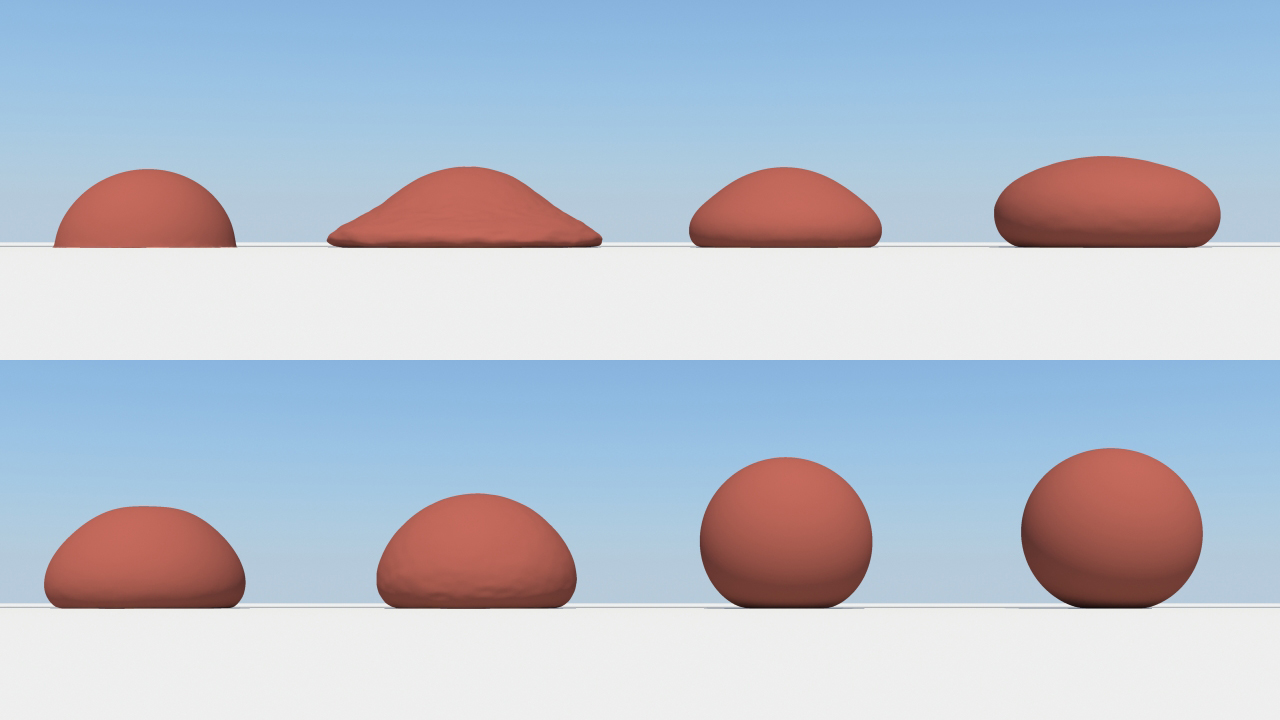
\includegraphics[width = 0.5 \linewidth]{translation/7.png}
  \caption{
    通过不同重量的体积保持约束和应变约束组合,可以模拟不同类型的体积物体材料。
  }
  \label{fig:translation-7}
\end{figure}

\subsection{基于范例的仿真}

基于范例的仿真允许通过提供一些材料应该遵循的变形范例来模拟艺术性的弹性材料行为[Martin et al. 2011; Koyama et al. 2012; Jones et al. 2013]。我们使用一个与公式\eqref{eq:translation-15}类似的能量,定义在3-流形表面上,如下所示:
\begin{equation}
  E(\vb{f}, \vb{R}, \vb{w}) = \frac{w}{2} \int_S \norm{\grad_S{\vb{f}} - \vb{R} \grad_S{\vb{h}(\vb{w})}}_F^2 + \delta_{SO(3)}(\vb{R}) \dd{V}
  \label{eq:translation-17}
\end{equation}
其中$\vb{h}(\vb{w})$是由范例定义的参数化的静止形状。我们将静止形状表述为$\vb{h}(\vb{w}) = \vb{g} + \sum_i w_i(\vb{R}_i \vb{g}_i - \vb{g})$,其中$\vb{g}_i$定义为范例的分段线性坐标函数,$\vb{R}_i$是预先计算的旋转矩阵,逐点定义,使其局部旋转$\vb{g}_i$以最佳对齐未变形状态$\vb{g}$,这与Koyama et al.[2012]的思想相似。

我们可以使用分段线性帽基函数离散化这个连续体能量,导出每个四面体的势能之和
\begin{equation}
  W(\vb{q}, \vb{R}, \vb{w}) = \frac{w}{2} V \norm{\vb{X}_{\vb{f}} \vb{X}_{\vb{g}}^{-1} - \vb{R} \vb{X}_{\vb{h}}(\vb{w}) \vb{X}_{\vb{g}}^{-1}}_F^2 + \delta_{SO(3)}(\vb{R})
  \label{eq:translation-18}
\end{equation}
其中$\vb{X}_{\vb{h}}(\vb{w}) = \vb{X}_{\vb{g}} + \sum_i w_i(\vb{R}_i \vb{X}_{\vb{g}_i} - \vb{X}_{\vb{g}}$)。请注意,范例权重$\vb{w}$可以在每个元素上局部定义,也可以全局定义,分别导致局部或全局的变形耦合。在图~\ref{fig:translation-8}中可以找到使用此约束的三辆相撞汽车的范例。

\begin{figure}
  \centering
  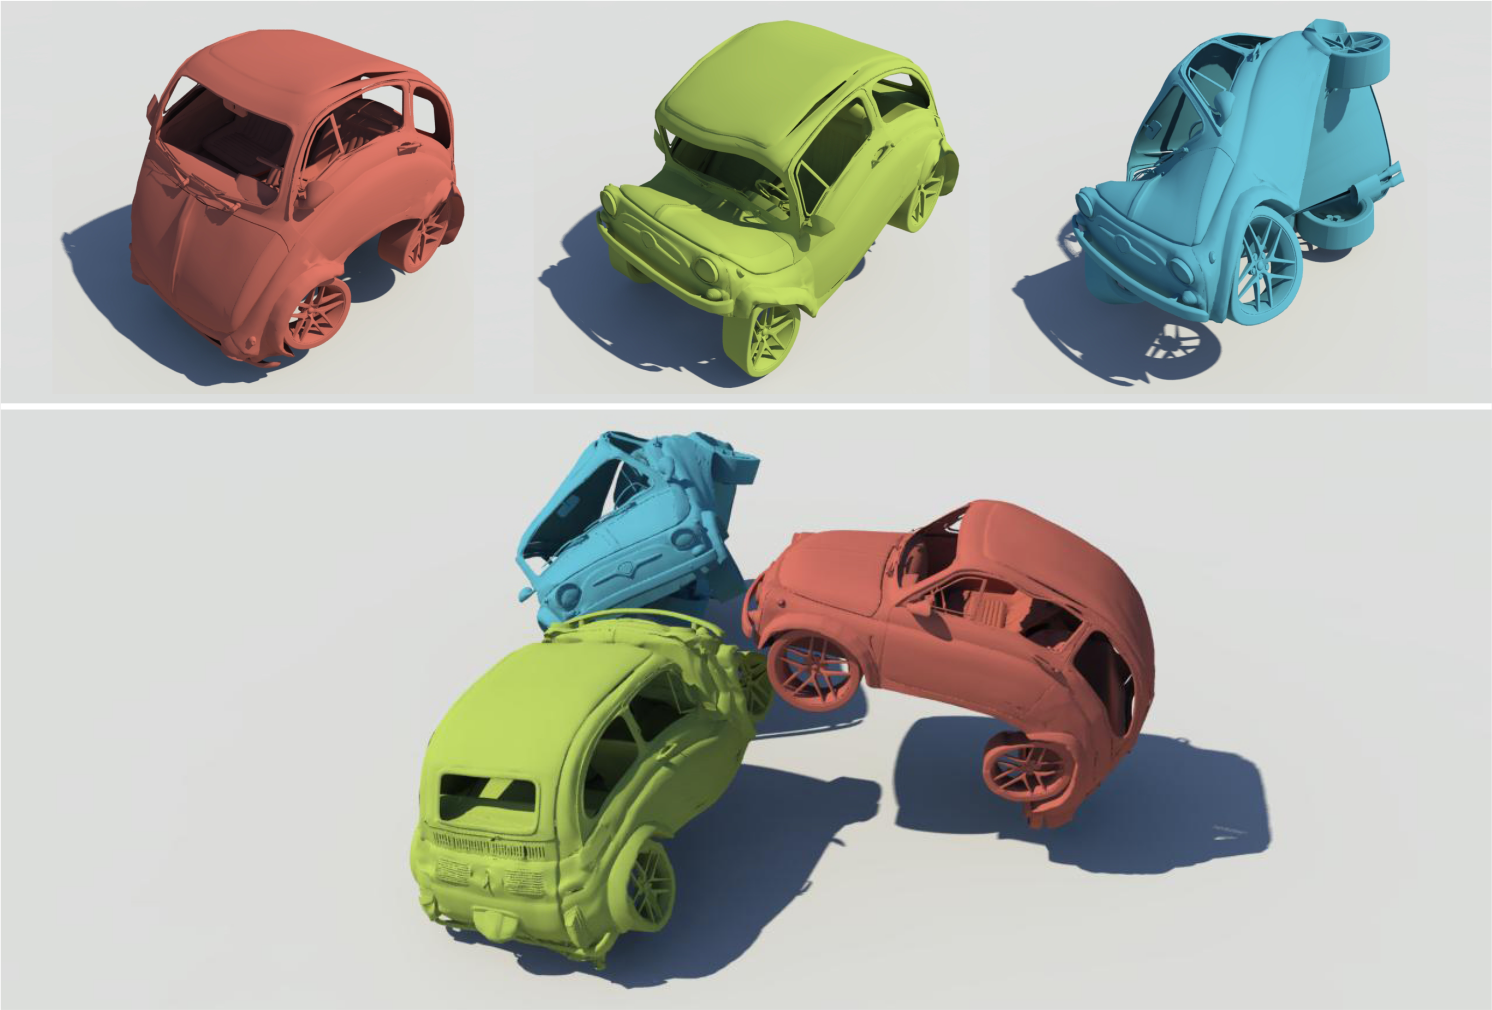
\includegraphics[width = 0.5 \linewidth]{translation/8.png}
  \caption{
    使用基于范例的约束将变形范例(上图)添加到模拟中,可以模拟复杂的艺术材料。在这个场景中,三辆汽车相撞,并按照规定的范例(下图)以卡通的方式作出反应。
  }
  \label{fig:translation-8}
\end{figure}

\subsection{弯曲}

\paragraph{连续体能量。}

薄壳和薄板通常使用基于边缘横跨角度的弯曲能进行模拟[Grinspun et al. 2003]。更近期地,已经提出了高效的模型来模拟不可伸展表面的弯曲,这些模型将Laplace-Beltrami算子与平均曲率法向量联系起来[Bergou et al. 2006; Garg et al. 2007]。我们引入了一个测量绝对平均曲率平方差的弯曲能
\begin{equation}
  E(\vb{f}) = \frac{w}{2} \int_S \pqty{\abs{H_{\vb{f}}} - \abs{H_{\vb{g}}}}^2 \dd{A}
  \label{eq:translation-19}
\end{equation}
其中$H_{\vb{f}}$ 和 $H_{\vb{g}}$分别是变形和未变形表面的平均曲率函数。对于等距变形(不可伸展表面),我们可以使用辅助旋转矩阵重写能量为
\begin{equation}
  E(\vb{f}, \vb{R}) = \frac{w}{2} \int_S \norm{\Delta_S{\vb{f}} - \vb{R} \Delta_S{\vb{g}}}_F^2 + \delta_{SO(3)}(\vb{R}) \dd{A}
  \label{eq:translation-20}
\end{equation}
其中$\Delta_S$是定义在流形表面$S$上的Laplace-Beltrami算子。这是因为平均曲率向量等于应用于坐标函数的表面的Laplace-Beltrami算子。对于等距变形,Laplace-Beltrami算子不会改变,因此可以在未变形表面上定义。请注意公式\eqref{eq:translation-20}与公式\eqref{eq:translation-15}是多么相似,将梯度替换为Laplace-Beltrami算子。因此,将应变限制和基于范例的概念应用于弯曲能也是有可能的。

\paragraph{离散势能}

如果$S$是一个2维单纯复形,公式\eqref{eq:translation-20}可以使用分段线性帽函数基进行离散化,从而得到每个顶点的势能形式为
\begin{equation}
  W(\vb{q}, \vb{R}) = \frac{w}{2} A \norm{\vb{X}_{\vb{f}} \vb{c} - \vb{R} \vb{X}_{\vb{g}} \vb{c}}_2^2 + \delta_{SO(3)}(\vb{R})
  \label{eq:translation-21}
\end{equation}
其中$A$是顶点的Voronoi面积,$\vb{X}_{\vb{f}}$和$\vb{X}_{\vb{g}}$分别包含了顶点在当前配置和静止配置下的一环边。向量$\vb{c}$存储了除以Voronoi面积的共同余切权重[Botsch et al. 2010]。图~\ref{fig:translation-9}中展示了一个弯曲约束的例子。如附录中所示,这种弯曲约束允许非常高效的局部求解,因为它可以仅仅通过对变形配置的平均曲率向量进行简单的归一化来实现。

\begin{figure}
  \centering
  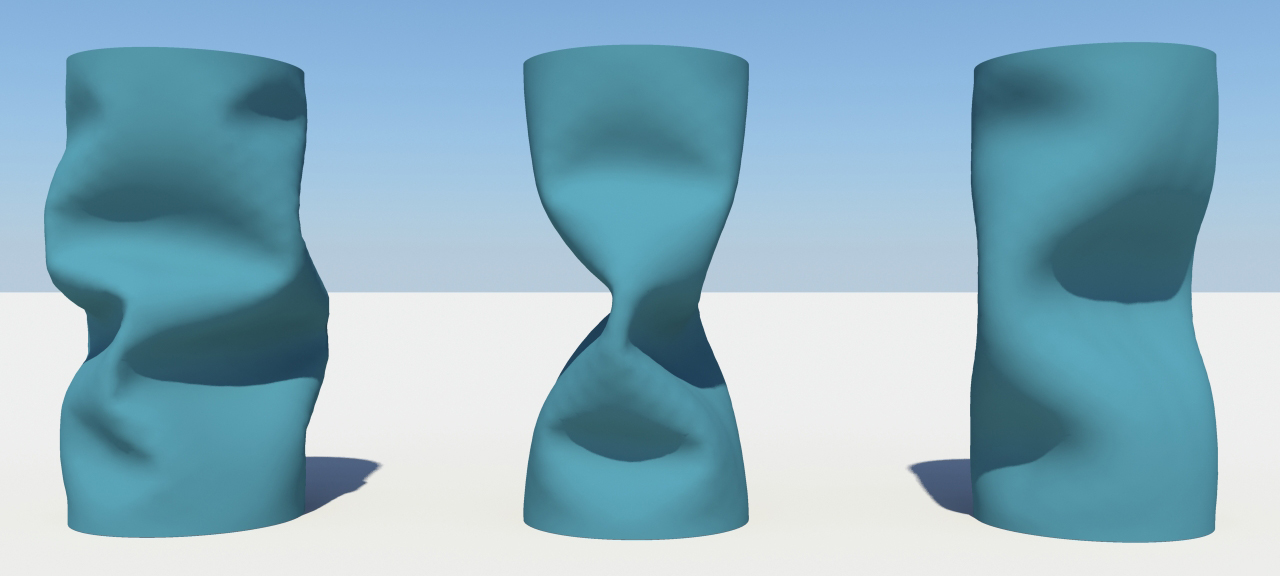
\includegraphics[width = 0.5 \linewidth]{translation/9.png}
  \caption{利用从左到右递增的弯曲重量模拟薄壳圆柱体。当圆柱体受到压缩时,会出现不同频率的屈曲模式。}
  \label{fig:translation-9}
\end{figure}

\section{离散约束}

上一节中从连续体能量导出的约束允许我们模拟多种多样的弹性体。对于实际的动画系统来说,其他约束同样重要。我们直接将这些约束建模为离散约束。

\paragraph{位置约束。}

如前所述,可以通过在公式\eqref{eq:translation-7}中简单选择$\vb{A}_i = \vb{B}_i = \vb{I}$来直接约束单个自由度。然后,可以通过定义约束集为期望的目标位置来实现\emph{Dirichlet边界条件},以便固定对象或创建可交互锚点。

\paragraph{碰撞。}

以隐式方式处理碰撞天然适合于我们的通用求解器中,并且允许在碰撞解决过程中尊重动量平衡和内部约束。当检测到碰撞时,我们动态地添加新的单侧平面约束。对于位置约束,我们再次在公式\eqref{eq:translation-7}中选择$\vb{A}_i = \vb{B}_i = \vb{I}$。对于发生碰撞的点$\vb{q}_c$,我们首先找到最近的表面点$\vb{b}$和法向$\vb{n}$,定义一个碰撞平面,使得约束集$\vb{C}$定义为半空间$\vb{n}^T (\vb{q} - \vb{b}) \geqslant 0$。在局部步骤中,投影到这个半空间是平凡的,因为它要么是一个平面投影,要么是恒等映射。请注意,单向定义碰撞约束允许我们克服在隐式碰撞处理中常见的粘附问题。类似于PBD,我们通过在更新速度时改变碰撞顶点的速度来处理摩擦和恢复力。一个简单的阻尼模型也可以通过过滤速度来实现[Müller et al. 2007]。

\paragraph{更多约束。}

一般类型的几何约束,例如使用铰链角度的弯曲约束[Bender et al. 2013],可以轻松地并入到我们的求解器中。局部求解可以通过最小化公式\eqref{eq:translation-7}来通用地执行,通过辅助变量。对于许多几何约束,可以找到这种最小化的封闭形式解[Bouaziz et al. 2012]。如果不存在封闭形式解,优化可以使用序列二次规划(SQP)[Nocedal and Wright 2006]来解决。如第~\ref{sec:translation-gauss-seidel-solver}节所示,对于$\vb{A} = \vb{B} = \vb{M}^{\frac{1}{2}}$的情况,SQP的一步与PBD更新类似[Bender et al. 2013]。

\section{实验结果}

\subsection{通用性}

我们的求解器不依赖于任何特定类型的约束,并且能够在相同的设置中处理各种各样的几何约束,这使得使用单一求解器模拟复杂场景成为可能,并且还能以隐式的方式鲁棒地处理对象间的交互作用。在图~\ref{fig:translation-1}中,我们展示了一个包含不同约束类型的复杂场景,其中的对象也是相互耦合的。例如,树和房子是用体积应变约束来建模的,而晾衣绳、布料、草和树叶则使用边缘应变和弯曲约束。

\paragraph{衣物和壳体。}

在图~\ref{fig:translation-10}中,我们简单地使用边缘应变约束来模拟海盗旗的行为。风力作为风向和三角形法线的函数被添加。当风力过强时,海盗旗会被撕裂。这是通过在应变超过一定阈值时移除边缘约束来实现的。可以使用限制三角形应变结合弯曲约束来模拟可以承受小到中等程度拉伸的更复杂的布料(见图~\ref{fig:translation-6})。通过改变应变和弯曲约束的权重,可以模拟其他类型的材料,如薄板和薄壳。在图~\ref{fig:translation-9}中,我们可以看到一个从顶部压缩的薄圆柱体,由于应变和弯曲约束刚度比例的不同,展现出不同的屈曲模式。

\begin{figure}
  \centering
  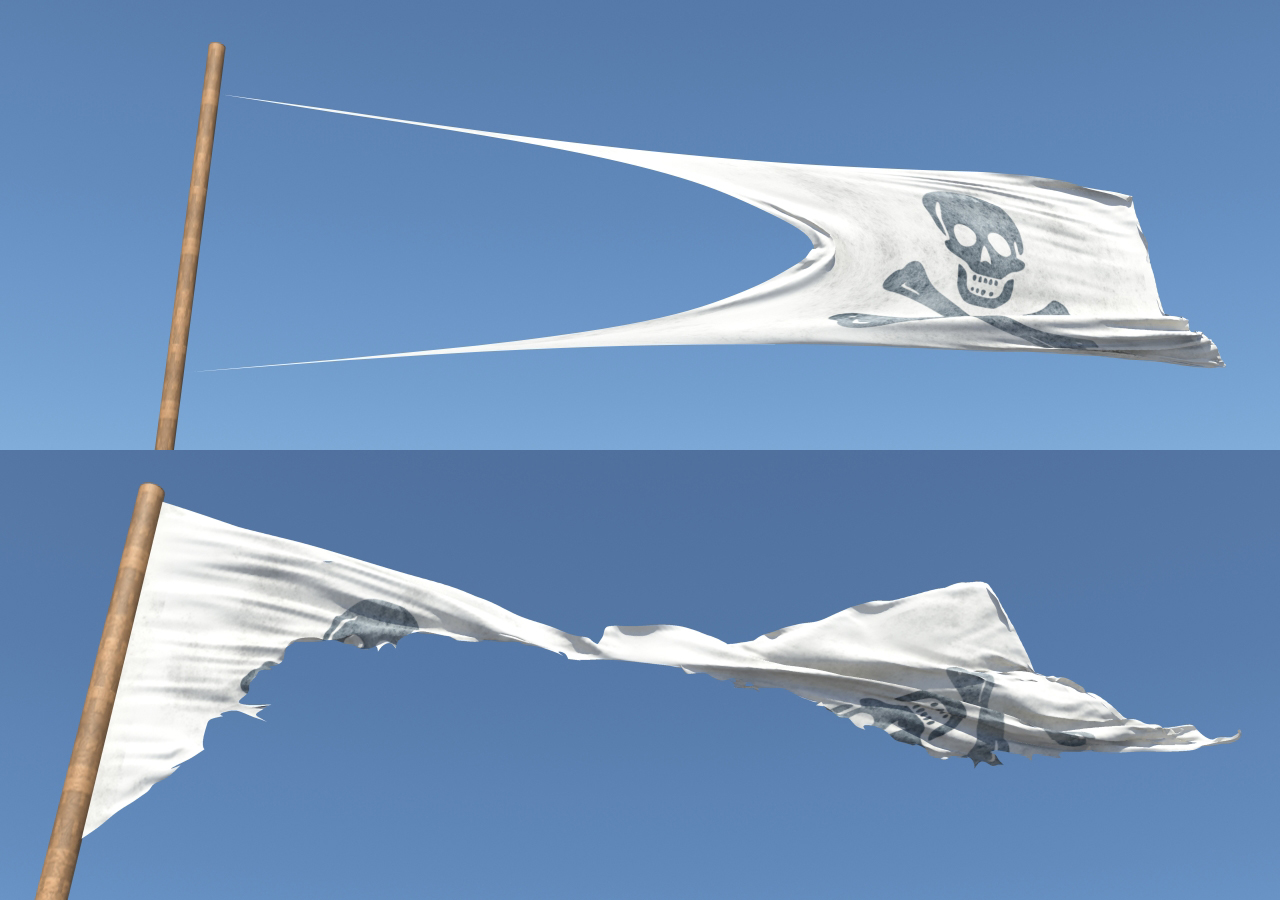
\includegraphics[width = 0.5 \linewidth]{translation/10.png}
  \caption{
    即使在极端风力作用下,我们的投影隐式求解器仍然保持稳定。求解器在每次迭代中弱化能量,使得任何安全措施都变得不必要(上图)。海盗旗在实时中被风撕裂,使用动态更新的约束(下图)。
  }
  \label{fig:translation-10}
\end{figure}

\paragraph{固体和基于范例的模拟。}

我们通过在四面体网格上应用应变和体积约束来模拟固体。如图~\ref{fig:translation-7}所示,不同类型的材料应变约束在我们的局部/全局求解器中进行了1次、10次和20次迭代模拟。值得注意的是,仅经过10次迭代,我们的方法看起来与使用牛顿法计算的收敛解非常相似,但计算成本只是一小部分。

通过改变这些约束的权重组合可以模拟不同的材料。虽然我们不能模拟任意的非线性材料,但我们能够通过结合弱应变约束和更强的限制应变约束来近似一些非线性行为。然后,当材料小变形时是柔软的,而当变形达到应变限制时,第二个约束变得活跃(见随附视频)——这是非线性材料模型通常模拟的行为。结合不同的二次势能已经在[Harmon et al. 2009]中用于碰撞处理,但也非常适合我们的框架来模拟非线性材料行为。

我们的公式也可以用于基于范例的体积网格模拟。这允许对物理模拟进行艺术性控制。在图~\ref{fig:translation-8}中,三辆汽车在碰撞后以卡通化的方式根据输入范例变形。类似于[Martin et al. 2011],汽车表面被嵌入到体积网格中,然后使用我们的求解器进行变形。

\subsection{鲁棒性和简单性}

我们方法的一个重要优势是数值稳定性。在图~\ref{fig:translation-10}中,我们展示了即使在极端力的作用下,我们的求解器也能保持鲁棒。同样地,我们的方法在网格元素退化的情况下也能保持可靠。这一点可以在压缩在两个平面之间的球体的模拟中看到(参见随附视频)。我们方法的唯一要求是输入模型的网格元素必须表现良好,以便计算原始流形的梯度和Laplace-Beltrami算子的离散化。

我们通过在算法~\ref{alg:translation-1}中展示我们的优化过程来说明我们方法的简单性。通过移除第~\ref{alg:translation-1L7}行并在第~\ref{alg:translation-1L5}行中将$\vb{p}_i$改为$\vb{q}_{n + 1}$,我们能够完全恢复原始PBD算法[Müller et al. 2007]的结构。此外,注意到引入一个新的约束只需要定义在局部求解中使用的约束投影(如果已知则为精确的,如果不知道则为[Müller et al. 2007]中给出的一般近似投影方案)以及适当的二次距离度量(矩阵$\vb{A}_i$和$\vb{B}_i$)的定义。

\subsection{准确性与性能}

\paragraph{与牛顿法的比较。}

在图~\ref{fig:translation-12}中,我们比较了我们的局部/全局求解器与牛顿法在求解公式\eqref{eq:translation-15}的离散化时的性能,其中$M = SO(3)$,类似于[Chao et al. 2010]。如图~\ref{fig:translation-12}所示,局部/全局方法在迭代次数上收敛得更慢。这是完全合理的,因为牛顿法表现出二次收敛,而局部/全局求解器(块坐标下降法)具有线性收敛。然而,当我们从计算时间的角度来看收敛性时,我们注意到我们的方法对于交互式应用来说比牛顿法更快。大约30次局部/全局迭代可以在1次牛顿迭代的时间内完成。这是因为在每次牛顿迭代中都需要重新计算Hessian矩阵,因此需要解一个新的线性系统。

此外,在图~\ref{fig:translation-11}和随附的视频中,我们观察到大约10次迭代后,模拟的效果在视觉上与使用牛顿法收敛的结果相似,这使得我们的方案成为实时应用的更好选择,其中高精度不是主要关注点。在几何处理和模拟中使用的一些先前的局部/全局求解器已经观察到了这种行为[Myles and Zorin 2012; Liu et al. 2013]。注意,对于第~\ref{sec:translation-continuum-based-constraints}节中提出的连续体能量实现牛顿法并非易事,因为需要对SVD[McAdams et al. 2011]进行微分,并且在每个时间步都需要计算新的Hessian矩阵。此外,优化中需要集成一些保护措施,因为Hessian矩阵可能变得不定,还需要一个线搜索过程来避免超调。

\begin{figure}
  \centering
  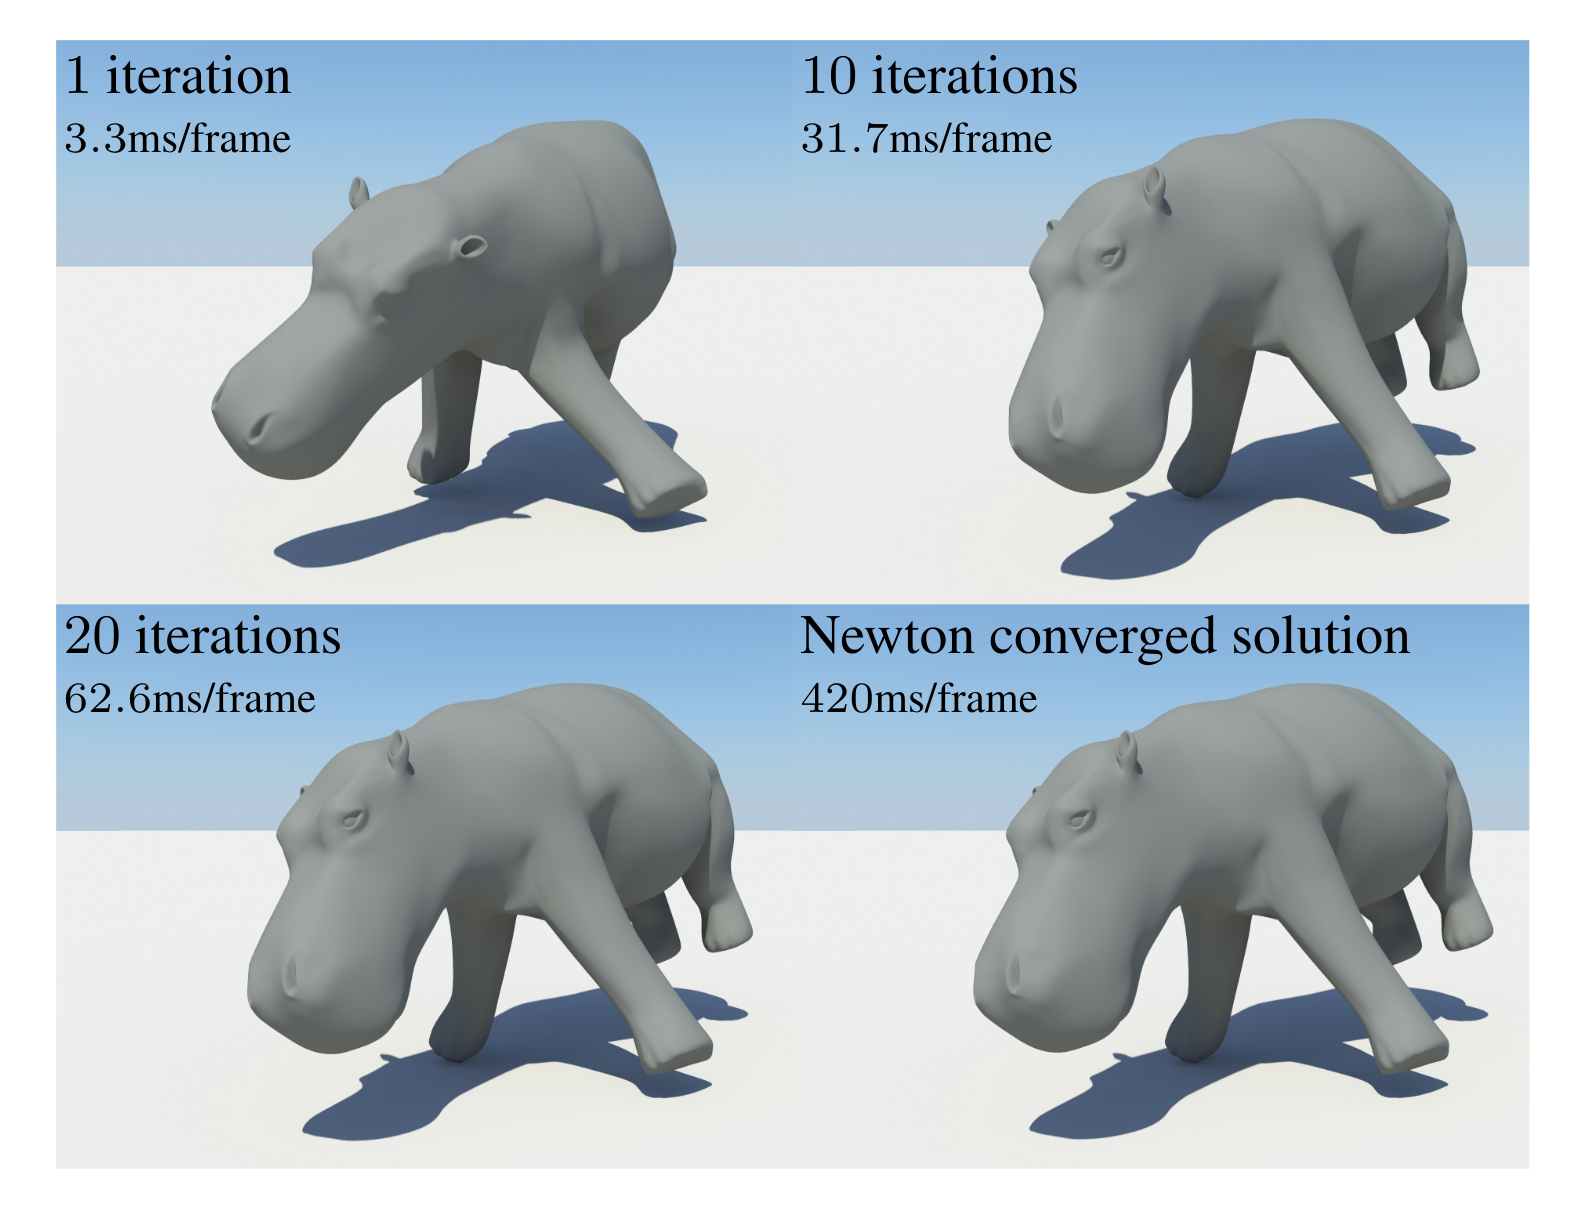
\includegraphics[width = 0.5 \linewidth]{translation/11.png}
  \caption{
    我们使用局部/全局求解器对这只具有\num{7161}个自由度和\num{8406}个应变约束的体积河马进行了1、10和20次迭代模拟。有趣的是,经过10次迭代后,我们的方法与使用牛顿法计算出的收敛解非常相似,而计算成本仅为牛顿法的一小部分。
  }
  \label{fig:translation-11}
\end{figure}

\begin{figure}
  \centering
  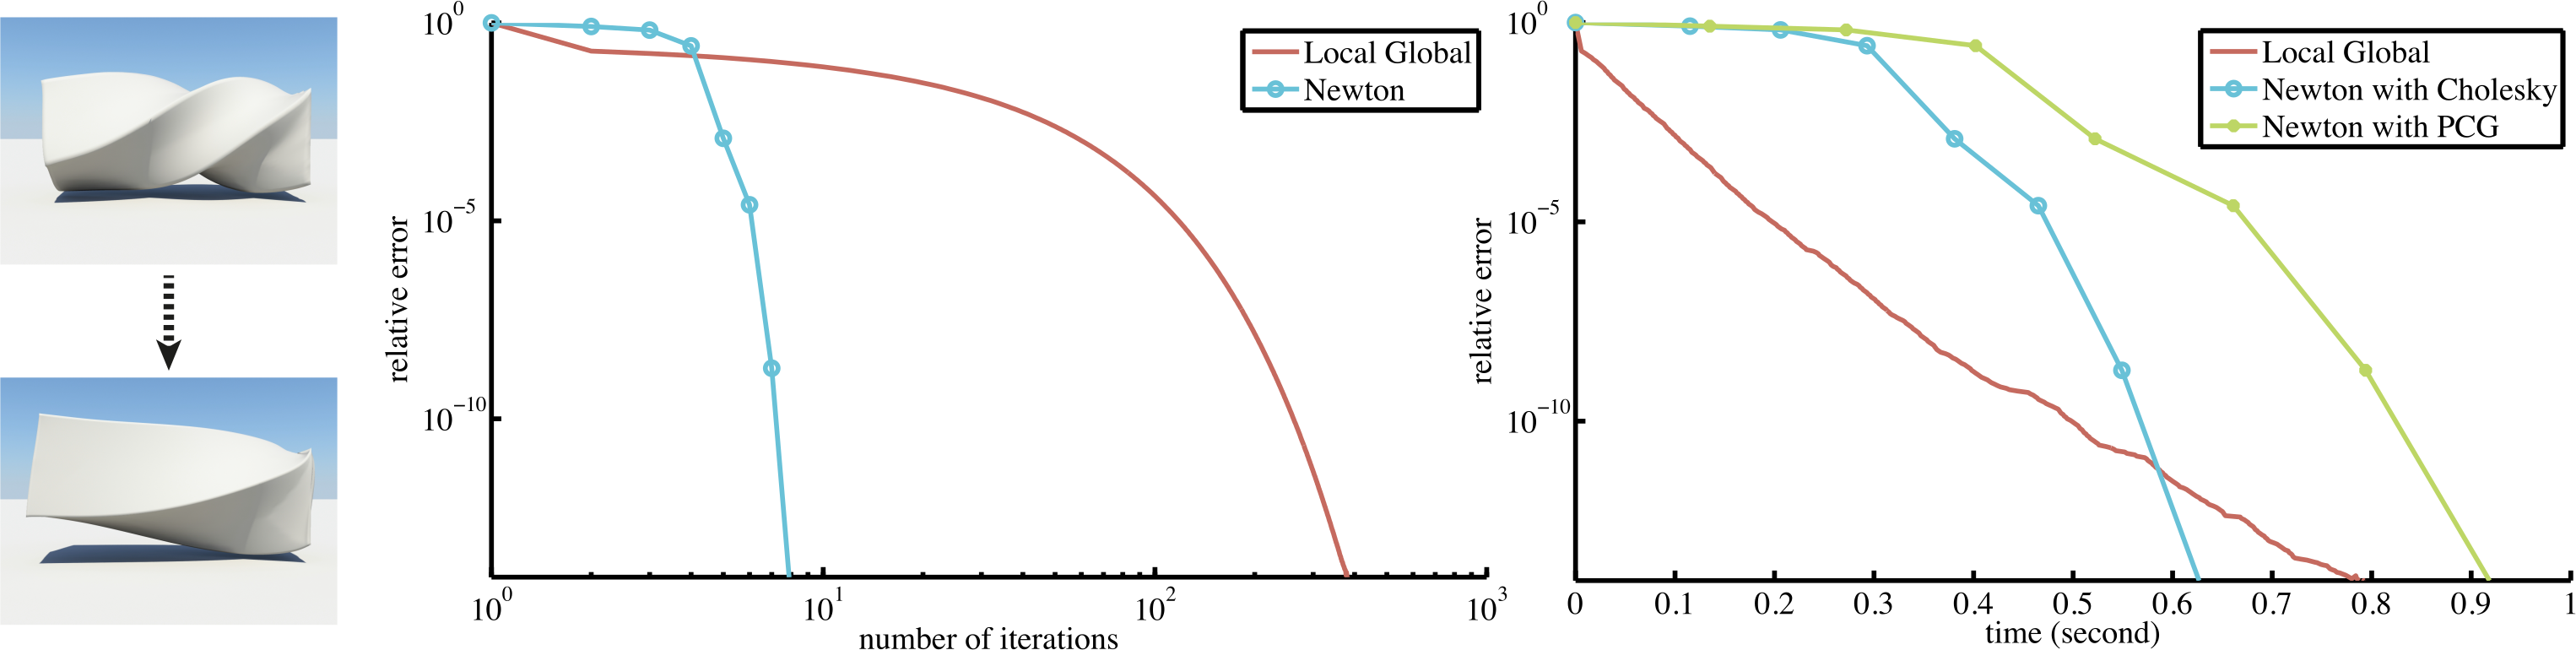
\includegraphics[width = 0.5 \linewidth]{translation/12.png}
  \caption{
    通过比较相对误差随迭代次数的减少,我们观察到牛顿法比我们的局部/全局方法收敛得更快。然而,这并不反映每次迭代的成本,因为每次牛顿迭代都需要求解一个变化的线性系统。观察相对误差随计算时间的减少,我们注意到我们的局部/全局方法在相对误差达到\num{e-10}时表现出更好的性能,这使得我们的方法对于交互式应用特别有吸引力。在这些曲线中,相对误差定义为相对于最优解的归一化误差$(\epsilon(\vb{q}_i) - \epsilon(q*)) / (\epsilon(\vb{q}_0) - \epsilon(\vb{q}^*))$,并且是针对一个扭曲条例子(左)进行测量的,该例子具有\num{4290}个自由度和\num{4099}个四面体应变约束。
  }
  \label{fig:translation-12}
\end{figure}

\paragraph{与基于位置的动力学的比较。}

我们还将我们的方法与使用边应变约束的PBD进行了比较。如第~\ref{sec:translation-position-based-dynamics-view}节所解释的,PBD不包括动量约束,这使得材料刚度依赖于迭代次数。这可以在随附的视频和图~\ref{fig:translation-4}中看到,对于不同数量的迭代,PBD模拟的材料刚度发生了巨大变化。而在我们的方法中,材料刚度与迭代次数的依赖性要小得多。

\paragraph{网格独立性}

在第~\ref{sec:translation-continuum-based-constraints}节中,我们提出了一组从连续体能量中派生出的新约束。如图~\ref{fig:translation-5}所示,这些新约束允许我们的求解器在不同的分片单纯形近似同一底层表面的情况下,保持变形行为的一致性。这对于计算机图形应用和交互式环境来说是一个重要的特性,因为在开发过程中网格分辨率可能会频繁变化,而且为了提高性能,广泛使用几何细节层次。PBD方法缺乏收敛性,由于材料行为依赖于底层网格和迭代次数的数量,这使得正确处理几何细节层次变得困难[Häggström 2009]。

\section{实现}

本文提出的完整框架是用C++实现的。我们使用OpenMP来并行化局部步骤,并且通过预先对线性系统进行稀疏Cholesky分解,然后并行地对$x$、$y$和$z$坐标进行三次回代,从而并行解决全局步骤。动态约束通过对线性系统进行秩的更新和降级来处理。我们使用Eigen库(eigen.tuxfamily.org)进行密集和稀疏的线性代数计算。我们使用标准的单纯形质量离散化[Hughes 2000]或其集中版本来计算质量矩阵,两者之间没有明显差异。

\paragraph{计时。}

对于中等大小模型的模拟(\SI{< 30}{k}约束和\SI{< 30}{k}自由度),通常\numrange{5}{10}次迭代就足够了。每次迭代\qtyrange{1}{6}{\milli\second},这使得在MacBook Pro 2.7 GHz Intel Quad-core i7处理器和16GB内存的电脑上能够实现实时模拟。关于计时和网格的统计数据可以在随附的视频中找到。此外,随附的应用程序展示了在多个示例上的性能表现。

\section{局限与未来工作}

尽管我们的隐式Euler求解器既高效又稳健,但它表现出隐式阻尼效应。在不久的将来,我们计划将我们的方法扩展到辛积分器[Kharevych et al. 2006],这些积分器提供更好的能量行为。当优化提前终止时,也可以观察到阻尼现象。这是因为如果优化没有运行足够的迭代次数,外部力可能无法完全通过网格传播。在大型网格中,这种效应更加明显,因为需要更多的迭代才能收敛。作为未来的工作,我们希望通过实现我们代码的GPU版本来提高求解器的速度,并专注于拓扑变化(切割、断裂)导致的动态变化约束。虽然在GPU上解决局部步骤仍然简单,但全局系统正在变化,使得高效解决它变得更加复杂。如果我们想将我们的方法扩展到类似[Macklin and Müller 2013]的流体模拟,那么这个问题会变得更加突出,因为邻域关系总是在变化。

我们为了简单和效率而牺牲了硬约束。以柔性方式处理所有约束,使我们能够以统一且有效的方式处理它们。然而,在某些情况下,能够强制执行硬约束,例如用于碰撞处理或边界条件,将是有利的。硬约束仍然可以通过增加约束的权重来近似。然而,这可能会降低线性系统的条件,并可能导致锁定伪影。

另一个有趣的进一步研究领域是扩大我们的约束集。我们想要探索的一个方向是模拟更复杂的变形行为,如各向异性和非线性材料。此外,将刚体集成到同一模拟框架中也将是有吸引力的。

\section{结论}

我们引入了一种新的基于隐式约束的求解器,用于实时模拟。我们的方法基于物理系统的抽象、基于约束的描述,使得我们的方法在用于模拟各种不同几何形状和材料方面具有普遍性。为了解决约束问题,我们应用了一个局部/全局求解器,它保证能够弱化地降低能量,从而无需任何安全保护措施,赋予了我们的方法以鲁棒性。我们简单的基于约束的公式只需要为给定的约束定义一个投影算子(局部求解),这使得它非常容易实现,并且很容易将新模型引入求解器。此外,全局求解只需要求解一个线性系统,如果约束数量保持不变,那么系统矩阵是常数,从而导致高效的计算。由于局部求解的独立性,这种方法也非常适合并行处理,进一步提升了性能。我们从连续体能量直接导出了一系列广泛的约束,通过适当的离散化使得求解器对于具有不同分辨率的非均匀网格化具有鲁棒性。考虑到这些特点,我们相信我们的方法在基于位置的模拟的简单性、通用性、鲁棒性和性能以及连续介质力学的严谨性和准确性之间取得了正确的平衡。我们认为这使得我们的方法适用于计算机图形学中许多实时和离线模拟的应用。

\paragraph{致谢。}

我们感谢James O'Brien、Adam Bargteil、Basil Fierz和Bernhard Thomaszewski的深入讨论以及审稿人的宝贵意见。我们感谢\emph{luismigabril}提供卡通房屋模型,感谢Daniel Grauer制作预告场景模型。我们还要感谢尤利-施瓦茨堡(Yuliy Schwartzburg)为配乐视频所做的解说。本研究得到了瑞士国家科学基金会20PA21L 129607号基金、欧盟第七框架计划(FP/20072013)/ERC补助金协议n. 257453: COSYM下的欧洲研究理事会以及美国国家科学基金会IIS-1350330 Career Award的支持。

\appendix

\section{局部求解}
\label{sec:translation-local-solves}

% 附录的内容。

\paragraph{应变。}

在局部步骤中,固定$\vb{q}$最小化$\vb{T}$时
\begin{equation}
  \min_{\vb{T}} \norm{\vb{X}_{\vb{f}} \vb{X}_{\vb{g}}^{-1} - \vb{T}}_F^2 + \delta_M(\vb{T})
  \label{eq:translation-22}
\end{equation}
该优化可以重新表述为
\begin{equation}
  \min_{\Sigma^*} \norm{\Sigma - \Sigma^*}_F^2 \qq{s.t.} \sigma_{\min} < \Sigma_{ii}^* < \sigma_{\max}
  \label{eq:translation-23}
\end{equation}
其中$\vb{X}_{\vb{f}} \vb{X}_{\vb{g}}^{-1} = \vb{U} \Sigma \vb{V}^T$ 且 $\vb{T} = \vb{U} \Sigma^* \vb{V}^T$。最优解可以计算为$\Sigma^*$,即将奇异值$\Sigma$限制在$\sigma_{\min}$和$\sigma_{\max}$之间。对于四面体,如果$\det(\vb{X}_{\vb{f}} \vb{X}_{\vb{g}}^{-1}) < 0$,则最后一个奇异值取反,以避免反射。

\paragraph{面积和体积。}

与应变约束类似,体积约束的局部最小化可以重新表述为
\begin{equation}
  \min_{\Sigma^*} \norm{\Sigma - \Sigma^*}_F^2 \qq{s.t.} \sigma_{\min} < \prod_i \Sigma_{ii}^* < \sigma_{\max}
  \label{eq:translation-24}
\end{equation}
这个问题可以进一步转换为
\begin{equation}
  \min_{\vb{D}} \norm{D}_2^2 \qq{s.t.} \prod_i (\Sigma_{ii} + \vb{D}_i) = \sigma
  \label{eq:translation-25}
\end{equation}
其中$\Sigma_{ii}^* = \Sigma_{ii} + \vb{D}_i$,当$\prod_i \Sigma_{ii}^* < \sigma_{\min}$时$\sigma = \sigma_{\min}$,当$\prod_i \Sigma_{ii}^* > \sigma_{\max}$时$\sigma = \sigma_{\max}$。这个受限最小化问题可以通过迭代求解一个二次规划问题来解决,通过线性化约束得到一个简单的更新规则
\begin{equation}
  \vb{D}^{k + 1} = \frac{\grad{\vb{C}(\vb{D}^k)}^T \vb{D}^k - \vb{C}(\vb{D}^k)}{\norm{\grad{\vb{C}(\vb{D}^k)}}_2^2} \grad{\vb{C}(\vb{D}^k)}
  \label{eq:translation-26}
\end{equation}
其中$\vb{C}(\vb{D}) = \prod_i (\Sigma_{ii} + \vb{D}_i) - \sigma$。

\paragraph{基于范例。}

我们通过迭代最小化$\vb{R}$和$\vb{w}$来解决优化问题
\begin{equation}
  \min_{\vb{R}, \vb{w}} \norm{\vb{X}_{\vb{f}} \vb{X}_{\vb{g}}^{-1} - \vb{R} \vb{X}_{\vb{h}}(\vb{w}) \vb{X}_{\vb{g}}^{-1}}_F^2 + \delta_{SO(3)}(\vb{R})
  \label{eq:translation-27}
\end{equation}
最小化$\vb{R}$是通过使用SVD跟随[Sorkine and Alexa 2007]来解决的,而求解$\vb{w}$对应于求解一个简单的线性系统。

\paragraph{弯曲。}

弯曲约束的局部求解可以表述为
\begin{equation}
  \min_{\vb{R}} \norm{\vb{v}_f - \vb{R} \vb{v}_g}_2^2 + \delta_{SO(3)}(\vb{R})
  \label{eq:translation-28}
\end{equation}
其中$\vb{v}_f = \vb{X}_f \vb{c}$且$\vb{v}_g = \vb{X}_g \vb{c}$。这相当于找到一个旋转$\vb{R}$,使得旋转后的向量$\vb{v}_g$最好地匹配向量$\vb{v}_f$。虽然$\vb{R}$可以使用SVD[Sorkine and Alexa 2007]找到,但这个问题有一个更简单的封闭形式解,即将$\vb{R} \vb{v}_g$替换为$\frac{\vb{v}_f \norm{\vb{v}_g}_2}{\norm{\vb{v}_f}_2}$。

% % 书面翻译的参考文献
% \bibliographystyle{unsrtnat}
% \bibliography{ref/appendix}

% 书面翻译对应的原文索引
\begin{translation-index}
\nocite{bouaziz2023projective}
\bibliographystyle{unsrtnat}
\bibliography{ref/appendix.bib}
\end{translation-index}

\end{translation}
  % 本科生:外文资料的书面翻译
% % !TeX root = ../thuthesis-example.tex

\chapter{补充内容}

附录是与论文内容密切相关、但编入正文又影响整篇论文编排的条理和逻辑性的资料,例如某些重要的数据表格、计算程序、统计表等,是论文主体的补充内容,可根据需要设置。

附录中的图、表、数学表达式、参考文献等另行编序号,与正文分开,一律用阿拉伯数字编码,
但在数码前冠以附录的序号,例如“图~\ref{fig:appendix-figure}”,
“表~\ref{tab:appendix-table}”,“式\eqref{eq:appendix-equation}”等。

\section{插图}

% 附录中的插图示例(图~\ref{fig:appendix-figure})。

\begin{figure}
  \centering
  
\includegraphics[width=0.6\linewidth]{example-image-a.pdf}
  \caption{附录中的图片示例}
  \label{fig:appendix-figure}
\end{figure}

\section{表格}

% 附录中的表格示例(表~\ref{tab:appendix-table})。

\begin{table}
  \centering
  \caption{附录中的表格示例}
  \begin{tabular}{ll}
    \toprule
    文件名          & 描述                         \\
    \midrule
    thuthesis.dtx   & 模板的源文件,包括文档和注释 \\
    thuthesis.cls   & 模板文件                     \\
    thuthesis-*.bst & BibTeX 参考文献表样式文件    \\
    thuthesis-*.bbx & BibLaTeX 参考文献表样式文件  \\
    thuthesis-*.cbx & BibLaTeX 引用样式文件        \\
    \bottomrule
  \end{tabular}
  \label{tab:appendix-table}
\end{table}

\section{数学表达式}

% 附录中的数学表达式示例(式\eqref{eq:appendix-equation})。
\begin{equation}
  \frac{1}{2 \uppi \symup{i}} \int_\gamma f = \sum_{k=1}^m n(\gamma; a_k) \mathscr{R}(f; a_k)
  \label{eq:appendix-equation}
\end{equation}

\section{参考文献}

附录中的参考文献示例(\cite{carlson1981two} 和 \cite{carlson1981two,taylor1983scanning,taylor1981study})。

\printbibliography


% 个人简历、在学期间完成的相关学术成果
% 本科生可以附个人简历,也可以不附个人简历
% % !TeX root = ../thuthesis-example.tex

\begin{resume}

  \section*{个人简历}

  197× 年 ×× 月 ×× 日出生于四川××县。

  1992 年 9 月考入××大学化学系××化学专业,1996 年 7 月本科毕业并获得理学学士学位。

  1996 年 9 月免试进入清华大学化学系攻读××化学博士至今。

  \section*{在学期间完成的相关学术成果}

  \subsection*{学术论文}

  \begin{achievements}
    \item Yang Y, Ren T L, Zhang L T, et al. Miniature microphone with silicon-based ferroelectric thin films[J]. Integrated Ferroelectrics, 2003, 52:229-235.
    \item 杨轶, 张宁欣, 任天令, 等. 硅基铁电微声学器件中薄膜残余应力的研究[J]. 中国机械工程, 2005, 16(14):1289-1291.
    \item 杨轶, 张宁欣, 任天令, 等. 集成铁电器件中的关键工艺研究[J]. 仪器仪表学报, 2003, 24(S4):192-193.
    \item Yang Y, Ren T L, Zhu Y P, et al. PMUTs for handwriting recognition. In press[J]. (已被Integrated Ferroelectrics录用)
  \end{achievements}

  \subsection*{专利}

  \begin{achievements}
    \item 任天令, 杨轶, 朱一平, 等. 硅基铁电微声学传感器畴极化区域控制和电极连接的方法: 中国, CN1602118A[P]. 2005-03-30.
    \item Ren T L, Yang Y, Zhu Y P, et al. Piezoelectric micro acoustic sensor based on ferroelectric materials: USA, No.11/215, 102[P]. (美国发明专利申请号.)
  \end{achievements}

\end{resume}


% 指导教师/指导小组评语
% 本科生不需要
% % !TeX root = ../thuthesis-example.tex

\begin{comments}
  % \begin{comments}[name = {指导小组评语}]
  % \begin{comments}[name = {Comments from Thesis Supervisor}]
  % \begin{comments}[name = {Comments from Thesis Supervision Committee}]

  论文提出了……

\end{comments}


% 答辩委员会决议书
% 本科生不需要
% % !TeX root = ../thuthesis-example.tex

\begin{resolution}

  论文提出了……

  论文取得的主要创新性成果包括:

  1. ……

  2. ……

  3. ……

  论文工作表明作者在×××××具有×××××知识,具有××××能力,论文××××,答辩××××。

  答辩委员会表决,(×票/一致)同意通过论文答辩,并建议授予×××(姓名)×××(门类)学博士/硕士学位。

\end{resolution}


% 本科生的综合论文训练记录表(扫描版)
% \record{file=scan-record.pdf}

\end{document}
